% LaTeX šablona pro seminární a jiné práce, v1.0 (2011-05-29)
% Tomáš Pikálek <tpikalek@gmail.com>, http://www.tpikalek.net

% % % % % % % % % % % % % % % % % % % % % % % % % % % % 
% Před použitím doporučuji přečíst roubor README.TXT  %
% % % % % % % % % % % % % % % % % % % % % % % % % % % % 

% Toto je hlavní soubor, který obsahuje některé definice a základní kostru dokumentu
% Kvůli přehlednosti nedoporučuji do tohoto souboru psát samotný text práce
% Text práce rozdělte do více souborů (nejlépe ve více složkách), ty sem poté vložte

% Vždy se překládá pouze tento soubor, nikoliv soubory jednotlivé!
% Např. používáte-li program Texmaker, otevřete tento soubor a dejte Volby → Prohlásit současný dokument za hlavní dokument
% Poté můžete upravovat jednotlivé soubory a při spuštění překladu se vždy bude překládat tento soubor




% Typ dokumentu - doporučuji neměnit
% Tisknete-li oboustranně, první řádek zakomentujte nebo smažte a odkomentujte druhý řádek
\documentclass [a4paper,11pt,oneside,notitlepage,openright]{report} % Typ dokumentu - pokud tisknete jednostranně
%\documentclass [a4paper,11pt,twoside,notitlepage,openright]{report} % Typ dokumentu - pokud tisknete oboustranně


% Načte styly dokumentu
% Jestliže chcete ovlivnit vzhled dokumentu, upravte právě tento soubor
\usepackage{00-Styly/Styly}
\usepackage{00-Styly/kod}



% % % % % % % % % % % % % % % % % % % % % % % % % % % % % % % % % % % % % % % % % % % % % %
	\def \Jmeno{Středoškolská odborná činnost} % Typ práce
	\def \Kategorie{Obor SOČ: 02 fyzika} % Kategorie práce
	\def \NazevCJ{Návrh malé větrné turbíny} % Návrh malé větrné turbíny
	\def \NazevAJ{Design of small wind turbine} % Design of small wind turbine
	\def \Autor {Jan Mrázek} % Autor
	\def \Datum {Hulín 2012} % Místo a datum
	\def \Podepsano {14. května 2012} % Datum podpisu prohlášení
	\def \Skola {Gymnázium Kroměříž\\\small{Masarykovo náměstí 496, 767 01 Kroměříž}} % Škola
% % % % % % % % % % % % % % % % % % % % % % % % % % % % % % % % % % % % % % % % % % % % % %



% Nastavit autora a titulek pro PDF výstup
\author{\Autor}
\title{\Jmeno - \NazevCJ}


\begin{document}

% Titulní stránka
% Obsahuje školu, typ a název práce, místo, datum a autora
% Pokud Vaše škola požaduje specifickou titulní stranu, je třeba vyměnit
\pagestyle{empty}

\begin{center}
	{\LARGE \textsc \Skola}\\

	\vspace{4cm}

	{
		\textbf {\Huge \Jmeno \\[1ex]}
		\textbf {\Large \Kategorie \\[8ex]}
		{\Huge \bf \NazevCJ \\[2ex]}
		{\LARGE \bf \NazevAJ}
	}

	\vfill

	{\large  \Datum \hfill Autor: \Autor}\\[6ex]

	\newpage
\end{center}
\cleardoublepage

% Nastavit prázdné stránky a číslování na římské číslice
% Toto se použije pro strany, které jsou před samotnou prací
\pagestyle{plain}
\pagenumbering{Roman}

% Prohlášení
% Následující soubor upravte, pokud nevyhovuje požadavkům
\vfill

\vglue 13cm

\section*{Prohlášení}

\begin{spacing}{1.3}
	 Prohlašuji, že jsem svou práci vypracoval samostatně, použil jsem pouze podklady (literaturu, software, atd.) uvedené v této práci a postup při zpracování a dalším nakládání s prací je v souladu se zákonem č. 121/2000 Sb., o právu autorském, o právech souvisejících s právem autorským a o změně některých zákonů (autorský zákon) v~platném znění. 
\end{spacing}

\vspace{1.5cm}

V~Hulíně dne \Podepsano

\begin{flushright}
	\vspace{-1.5cm}
	\begin{tabular}{p{3.5cm}}
		\hspace{0.8cm}
\includegraphics[height=1cm]{00-Hlavicka/podpis.png}
		\\
		\hline
		\hspace{1cm} podpis
	\end{tabular}
	\hspace*{0.5cm}
\end{flushright}

\newpage

% Poděkování
% Upravte následující soubor
\vfill

\vglue 14cm

\section*{Poděkování}

\begin{spacing}{1.3}
Chtěl bych poděkovat zejména mému otci, který mě v~celém mém bádání podporuje a poskytuje mi pomoc v~konstrukčních stránkách celé stavby. 
\end{spacing}

\cleardoublepage

% Abstrakt
% Upravte následující soubor
% V tomto souboru je obstrakt
% Abstrakt by v práci měl být česky i anglicky
% Jestliže nemusíte mít anglický abstrakt, je možné jej odstranit

% Nastavit jiné odrážky pro klíčová slova
\renewcommand{\labelitemi}{--}

\section*{Abstrakt}\label{AbstraktCZ}

\begin{spacing}{1.3}
	Práce se zabývá aerodynamikou malých větrných turbín a zejména jejich návrhem. Popisuje návrh malé horizontální větrné turbíny o průměru 2,5~m. Zkoumá různé aspekty její účinnosti, zabývá se její startovatelností a omezením indukovaných ztrát.
	Práce dále popisuje také stavbu druhé menší turbíny založené na zjednodušeném výpočtu.
\end{spacing}

\section*{Klíčová slova}

\begin{itemize}
	\item turbína
	\item aerodynamika
	\item elektrárna
	\item domácí stavba
	\item vítr
\end{itemize}

\newpage

% Nastavit jako jazyk angličtinu
\begin{otherlanguage}{english}

\section*{Abstract}\label{AbstraktEN}

\begin{spacing}{1.3}
	The work deals with aerodynamics of small wind turbines and in particular with their design. It describes design of small wind turbine with a diameter of 2.5 m. It discusses aspects of its efficiency, startability and ways how to reduce induced losses.
	The work also describes construction of another, smaller, turbine based on simplified theory.

\end{spacing}

\section*{Keywords}

\begin{itemize}
	\item turbine
	\item aerodynamics
	\item power plant
	\item home construction
	\item wind
\end{itemize}

\end{otherlanguage}

% Nastavit původní odrážky
\renewcommand{\labelitemi}{\textbullet}
\cleardoublepage

% Originální zadání v PDF
% Jestlite máte originál zadání a máte jej v práci uvádět, zde jej můžete vložit jako PDF
% V opačném případě následující řádky smažte nebo zakomentujte
%
\includepdf{00-Hlavicka/Zadani.pdf}
%\cleardoublepage

% Posudek v PDF
% Jestliže máte na práci vypracovaný posudek, zde jej můžete vložit jako PDF
% V opačném případě následující řádky smažte nebo zakomentujte
%
\includepdf{00-Hlavicka/Posudek.pdf}
\cleardoublepage

% Obsah
\tableofcontents
\cleardoublepage

% Seznam obrázků
%\addcontentsline{toc}{chapter}{Seznam obrázků}
%\listoffigures
\cleardoublepage

% Seznam tabulek
%\addcontentsline{toc}{chapter}{Seznam tabulek}
%\listoftables
\cleardoublepage

% Nastavit normální číslování stránek
% Toto se použije na samotný text práce
\pagenumbering{arabic}
%\pagestyle{headings}
%\pagestyle{headings}




% Načíst soubory
% % % % % % % % % % % % % % % % % % % % % % % % % % % % % % % % % % % % % % % % % % % % % %
% Zde se načítají soubory s vlastním textem práce
% Doporučuji se držet výchozího schématu
% Je vhodné kvůli přehlednosti celou práci rozdělit do několika složek a souborů, každý zde pak vložit zvlášť
% U krátkých prací doporučuji nepoužívat části, ale dělit jen na kapitoly
		\chapter{Úvod}

	Větrné elektrárny jsou často diskutovaným tématem. Některým lidem se líbí, některým ne. Já sám se řadím mezi příznivce větrných elektráren. Jedná se o zajímavá zařízení se zajímavým technickým původem. Neberu je však jako hlavní a jediný zdroj energie. Považuji je spíše za ukázky technické zdatnosti lidstva.
	
	\section{Cíle práce}
		Díky mému zájmu jsem před několika lety začal sám v této oblasti experimentovat a zkoumat. Mnoho pokusů však bylo marných a neúspěšných. Doposud jsem zdaleka nedosáhl mých představ. Avšak za tu dobu jsem se jim přiblížil.
		
		Tato práce mapuje dva největší počiny v mém bádání – sestrojení první teorií podložené větrné turbíny a návrh nové, z ní vycházející, která zatím nebyla sestrojena.
		
		Mým cílem je sestrojit malou větrnou elektrárnu umístěnou na zahradě rodinného domku. Nechci však sestrojit ekonomicky rentabilní elektrárnu (takovou, která vyrobí elektřinu ve větší hodnotě, než stála její stavba). Vedou mě k tomu dva důvody – jednak elektrárnu stavím pro poznání, nikoliv pro zisk; ale hlavně je to pro malé elektrárny (průměr do 5 m) v podstatě nemožné (hlavně díky malé účinnosti profilů na malých rotorech, ale také díky tomu, že získaná energie roste se čtvercem poloměru rotoru). Chci sestrojit elektrárnu, která se bude snažit dosáhnout co největší účinnosti a bude aerodynamicky co nejdokonalejší.
		
		Proto jsem tuto práci zaměřil relativně úzce. Zaměřuji se zde pouze na návrh turbíny, nikoliv generátoru, regulačního systému a dalších. Záměrně zde také vynechávám pojednání o výběru stanoviště pro elektrárnu (protože nemám možnost si stanoviště vybírat). Díky mým požadavkům nedělám v mém návrhu kompromisy mezi komplikovaností výroby a získanou energií.
		
		Práci jsem rozdělil na dvě hlavní části. V části \ref{part:navrh} nejprve shrnuji teoretické poznatky, které byly doposud objeveny, o funkci větrných turbín. Na základě těchto poznatků pak dále popisuji návrh nové turbíny. Cílem bylo vytvořit CAD model turbíny, dle kterého bude tato turbína v~budoucnu vyrobena.
		V~části \ref{part:stavba} pak popisuji návrh a výrobu mé první turbíny, jejíž návrh byl teoreticky podložen. V~této práci ji označuji jako \uv{první prototyp}. Také zde uvádím zkušenosti s~jejím provozem.
	
	\section{Použité zdroje}
		\subsection{Literatura}
			Zdrojem pro jednotlivé teorie byla především kniha \cite{Rychetnik:Motory}. Ta poskytuje ucelený přehled základních poznatků a hlavně na rozdíl od ostatních knih, které jsem četl, tuto teorii vysvětluje, a nepopisuje pouze její aplikaci. Narazil jsem v ní však na několik nepřesností (např. překlepy ve vzorcích). Na tuto knihu mě nasměrovaly internetové stránky \cite{ve:ve}, které mi před několika lety poskytly počáteční impuls pro další bádání a stavbu.
			
			Údaje z této knihy jsem doplňoval několika informacemi z knihy \cite{Crome:Technika}. Na doplnění údajů o~různých osobnostech aerodynamiky jsem použil informace z Wikipedie.
			
			Data o aerodynamických profilech byla převzata ze stránek \cite{profil}.
			
		\subsection{Obrázky}
			Veškeré obrázky a fotografie jsou mé vlastní a byly vytvořeny pro účely této práce. Obrázky jsou často inspirovány obrázky z knihy \cite{Rychetnik:Motory}. Jsou doplněné, popř. krácené, o informace vhodné pro mé parafrázování teorie.
		\subsection{Software}
			Práce byla vysázena za pomoci \LaTeX u a šablony od Tomáše Pikálka\footnote{http://tpikalek.cz/latex/}. Pro nákres obrázků jsem použil program IPE\footnote{http://ipe7.sourceforge.net/}. Pro sestavení CAD modelu jsem použil studentskou verzi programu SolidWorks. Pro pomocné výpočty a tvorbu grafů jsem použil program Microsoft Excel. Na pomocné algebraické výpočty (např. derivace, úprava složitých výrazů pro zamezení chyb) jsem použil program Microsoft Mathematics\footnote{http://www.microsoft.com/download/en/details.aspx?id=15702}. Pro provedení aerodynamických simulací jsem použil studentskou verzi programu Autodesk Simulation Multiphysics\footnote{http://www.microsoft.com/download/en/details.aspx?id=15702}  z~programu Autodesk Club\footnote{http://www.autodeskclub.cz/student}. Pro vývoj a zkompilování pomocného programu pro výpočet turbíny jsem použil IDE Microsoft Visual C++ Express\footnote{http://www.microsoft.com/visualstudio/en-us/products/2010-editions/express}.

	\part{Návrh malé větrné turbíny}\label{part:navrh}
		%Vložení jednotlivých kapitol
%Výběr
	\chapter{Výběr typu turbíny}
	Prvním krokem pro návrh větrné turbíny je určení typu. Každý typ má své specifické charakteristiky s~výhodami a nevýhodami. V~této kapitole jsem stručně popsal jednotlivé typy větrných turbín a rozebral jejich výhody a nevýhody. Na závěr kapitoly jsem ze zjištěných poznatků vybral vhodný typ větrné turbíny.	
	\section{Typy větrných turbín}\label{sec:typy_turbin}
		Větrné turbíny se běžně rozdělují na 2 základní skupiny podle principu – na odporové a vztlakové \cite{Rychetnik:Motory}.
		
		Odporové turbíny jsou z~historického hlediska starší. Základním principem těchto turbín je plocha, která klade větru odpor. Na této ploše vzniká síla, která rotorem otáčí. Plocha se však musí dostávat zpět na výchozí polohu. Běžně se používají 2 řešení\cite{Rychetnik:Motory}:
		
		\paragraph{Odporová plocha má různý odpor}
			Odporová plocha má při různých směrech obtékání různý aerodynamický odpor. Typickým příkladem je klasický miskový anemometr, jehož lopatky mají tvar duté polokoule. Polokoule má z vypouklé strany mnohem menší odpor než ze strany s~dutinou. Díky tomu se může miskový anemometr otáčet dokola. Na podobném principu pracuje i Savoniův rotor, který používá různě tvarované válcové plochy.
		\paragraph{Odporová plocha je natáčena}
			Plocha je v závislosti na pozici rotoru a směru větru natáčena. Toto řešení může dosahovat větší účinnosti než předchozí řešení s různým aerodynamickým odporem, ale je mnohem komplikovanější na výrobu a návrh.
			
		\bigskip	
		Díky jednoduchému principu lze sestrojit širokou škálu větrných turbín rozličných tvarů pracujících na odporovém principu. Lze sestrojit jak rotory s horizontální osou (anglicky označované jako HAWT – horizontal axis wind turbine), tak i s osou vertikální (anglicky označované jako VAWT – vertical axis wind turbine)\cite{ve:ve}.
		
		Dnes jsou nejpoužívanější turbíny pracující na vztlakovém principu. Základním principem je vztlak vznikající na listech turbíny. Tyto turbíny se používaly několik stovek let u větrných mlýnů; teoretické poznatky o jejich funkci jsou však mnohem mladší. Teoretické základy pro stavbu těchto turbín položil až na začátku 20. století německý fyzik Albert Betz\cite{betz}. Své první poznatky shrnul v knize  \uv{Das Maximum der theoretisch möglichen Ausnutzung des Windes durch Windmotoren}\cite{betz}.
		
		Turbíny lze sestrojit jak v horizontálním provedení, tak i vertikálním. Vertikální provedení si nechal patentovat francouzský inženýr aerodynamiky Georges Jean Marie Darrieus\cite{dar}. Běžně se tento typ turbíny označuje jako Darrieova turbína, či jen Darrieus.
		
		Horizontální provedení se dnes nejčastěji využívá u velkých větrných elektráren díky relativně snadné možnosti regulace otáček (oproti rotoru Darrieus). Horizontální turbíny se také dříve používaly jako pumpy na vodu – známé mnohalopatkové \uv{americké větrné kolo}\cite{ve:ve}.
	\section{Výběr typu turbíny}
		V předchozí kapitole jsem záměrně vynechal porovnání jednotlivých turbín. V této kapitole bych chtěl jednotlivé typy navzájem porovnat a vybrat nejvhodnější pro můj návrh.
		
		Odporové turbíny vynikají jednoduchou konstrukcí. Základní typy (např. Savoniův rotor) nejsou příliš náročné na přesnost výroby. Jejich nevýhodou je však nižší účinnost – Savoniův rotor dosahuje maximální účinnosti 23~\%, běžně však méně \cite{Rychetnik:Motory}. Fungují pouze při nízké rychloběžnosti (poměr obvodové rychlosti vůči rychlosti větru; viz. dále kapitola \ref{kap:funkce1}). Díky tomu dosahují malých otáček, což je nevhodné pro potenciální výrobu elektrické energie.
		
		Vztlakové turbíny mají vyšší účinnost (až 48~\%, většinou okolo 35~\%) \cite{Rychetnik:Motory} a větší rozsah použitelné rychloběžnosti. Jsou proto vhodné jak např. pro pumpování vody (pomaloběžné rotory), tak i jako rychloběžné pro výrobu elektrické energie. Jejich nevýhodou je však relativně větší náročnost na přesnost výroby a potřebné teoretické znalosti.
		
		Vertikální umístění rotoru má oproti horizontálnímu umístění výhodu v~odstranění nutnosti natáčet rotor vůči větru, navíc jsou méně náchylné na turbulence a víry v okolí. Díky tomu jsou schopny pracovat i relativně nízko u země a nepotřebují tedy vysoký stožár\cite{Rychetnik:Motory}\cite{ve:ve}.
		
		Pro svůj návrh jsem se rozhodl pro vztlakovou horizontální turbínu. Vztlakové turbíny mají vyšší účinnost, jsou použitelné pro vyšší rychloběžnosti a také jsou technicky zajímavější než odporové. Při volbě mezi svislou a horizontální turbínou jsem se po dlouhém zvažování rozhodl pro horizontální. To i přes fakt, že turbína bude umístěna v~zástavbě, kde je turbulentní okolí. Tudíž lze podle výše uvedeného usuzovat, že je vhodnější vertikální turbína.
		
		Vedlo mě k tomu několik faktů; Darrieus není sám o sobě schopný rozběhu. Je mu nutno dodat počáteční rotaci. U~malých turbín se tento nedostatek řeší pomocným, např. Savoniovým, rotorem, který ji rozběhne. O alternativním způsobu rozběhu Darrieovi turbíny pojednává práce \uv{Self-starting Darrieus Wind Turbine}\footnote{Práci lze nalézt na http://www.webalice.it/acecere48/finalreport.pdf} z univerzity Dalhousie. Zde jsou listy turbíny rozděleny na 2 části, které se mohou od sebe rozevírat – při rozběhu jsou rozložené a pracují v odporovém režimu. Při dosažení daných otáček se listy opět složí a pracují ve vztlakovém režimu. Toto řešení je zajímavé, avšak klade ještě větší výrobní nároky – již tak tenké a dlouhé listy je nutno rozpůlit.
		
		Pro horizontální turbínu však hlavně rozhodly mé předchozí pozitivní zkušenosti ze stavby a provozu tohoto typu turbíny.
		

	\chapter{Teorie výpočtu}
\label{kap:teorie}
	V této kapitole bych rád čtenáře seznámil s teoretickými poznatky, ze kterých jsem při mém návrhu vycházel. Celá tato kapitola \ref{kap:teorie} je parafrázováním knihy \cite{Rychetnik:Motory} doplněné o některé mé postřehy a poznámky. Kapitola je rozdělena na dvě části – v první se zabývám teoretickou účinností větrných motorů. V druhé části popisuji funkci horizontální vztlakové turbíny a uvádím dva způsoby výpočtu.
	
	\section{Teoretická účinnost větrných turbín}\label{ucinnost}
	Jak jsem již zmínil v kapitole \ref{sec:typy_turbin}, základy funkce vztlakových turbín popsal Albert Betz. Ten odvodil maximální teoretickou účinnost větrných motorů. Na jeho počest je nazývána Betzova.
	
	Je několik různých způsobů výpočtů maximální účinnosti. Některé dávají vyšší a některé nižší hodnoty (např. maximální účinnost podle Sabinina je 68,7~\% \cite{Rychetnik:Motory}). Běžně se však v literatuře uvažuje právě Betzova účinnost. Tato účinnost je pouze teoretická. Skutečná účinnost je vždy značně nižší (aby se turbína mohla přiblížit ideální, nesměla by proudu vzduchu za ní udělovat rotační složku).
	V této kapitole bych rád ukázal, jak lze Betzovu účinnost odvodit. Odvození vychází z~obrázku~\ref{obr.rotor}:
	\begin{figure}[H]
		%\begin{center}
		\centering
			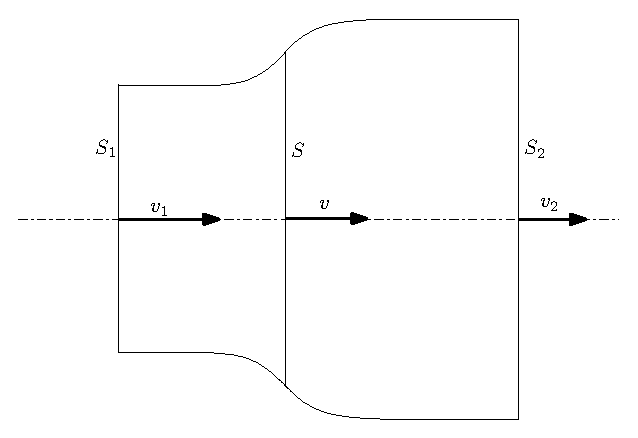
\includegraphics[]{obrazky/rotor}
	          %\input{obrazky/rotor2.ipe}
		\caption{Princip větrné turbíny. Proud vzduchu (v ploše $S_1$ s rychlostí $v_1$) vstupuje do roviny turbíny $S$. Zde je zpomalen a za rotorem vystupuje v ploše $S_2$ s rychlostí $v_2$. Inspirováno \cite{Rychetnik:Motory}.}
		\label{obr.rotor}
	    %\end{center}
	  \end{figure}
	
	Tento nákres znázorňuje proud vzduchu procházející rotorem. Za předpokladu, že se tento proud nemísí s okolním vzduchem, je soustava izolovaná a platí zde rovnice kontinuity \eqref{rov:1}\cite{Rychetnik:Motory}:
	
	\begin{equation}
		S_1 v_1 = Sv = S_2 v_2\label{rov:1}
	\end{equation}
	Poté lze za zákona zachování hybnosti odvodit axiální sílu $F_a$ působící na rotor \eqref{rov:2}\cite{Rychetnik:Motory}:
	\begin{eqnarray}
		\label{rov:2}
		\Delta p = p_1 - p_2 \nonumber \\
		F\Delta t=mv_1 - mv_2 \nonumber \\
		F\Delta t = \rho Sv\Delta t(v_1 - v_2) \nonumber \\
		F_a = \rho Sv(v_1 - v_2)
	\end{eqnarray}
	Z axiální síly $F_a$ lze spočítat i výkon turbíny \eqref{rov:3}\cite{Rychetnik:Motory}:
	\begin{equation}
		\label{rov:3}
		P = F_a v = \rho Sv^2 (v_1 - v_2)
	\end{equation}
	Výkon turbíny lze také spočítat i pomocí změny kinetické energie proudu vzduchu \eqref{rov:4}\cite{Rychetnik:Motory}:
	\begin{equation}
			\label{rov:4}
			P = \frac{\Delta E_k}{\Delta t} = \frac{1}{2} \rho Sv(v_1^2 - v_2^2)
	\end{equation}
	Porovnáním různě vyjádřeného výkonu z rovnice \ref{rov:3} a \ref{rov:4} vyplývá, že rychlost v rovině rotoru je aritmetickým průměrem rychlosti před a za rotorem \eqref{rov:5}\cite{Rychetnik:Motory}:
	\begin{equation}
			\label{rov:5}
			P_p = P_{E_k} \Rightarrow v=\frac{v_1 + v_2}{2}
	\end{equation}
	Díky tomuto poznatku lze vyjádřit axiální sílu $F_a$ i výkon $P$ pouze v závislosti na rychlosti proudu větru před a za rotorem\eqref{rov:6}\cite{Rychetnik:Motory}:
	\begin{eqnarray}
		\label{rov:6}
		F_a = \frac{1}{2}\rho S(v_1^2 - v_2^2) \nonumber \\
		P=\frac{1}{4}\rho S(v_1^2 - v_2^2)(v_1 + v_2)
	\end{eqnarray}
	Účinnost můžeme vyjádřit jako poměr výkonu turbíny a výkonu proudu vzduchu vstupujícího do turbíny vzduchu\eqref{rov:7}\cite{Rychetnik:Motory}. Výkon proudu vzduchu lze určit pomocí kinetické energie tohoto proudu.
	\begin{equation}
		\label{rov:7}
		\eta = \frac{\frac{1}{4}\rho S(v_1^2 - v_2^2)(v_1 + v_2)}{\frac{1}{2}\rho Sv_1^3}=\frac{(v_1^2 - v_2^2)(v_1 + v_2)}{2v_1^3}
	\end{equation}
	Pokud vyjádříme poměr rychlostí proudu vzduchu před a za rotorem následovně\eqref{rov:8}\cite{Rychetnik:Motory}:
	\begin{equation}
		\label{rov:8}
		k= \frac{v_2}{v_1}
	\end{equation}
	Lze rovnici \eqref{rov:7} zjednodušit na tvar \eqref{rov:9}
	\begin{equation}
		\label{rov:9}
		\eta = \frac{(k+1)(1-k^2)}{2}
	\end{equation}
	Derivací tohoto výrazu můžeme zjistit jeho maximum\eqref{rov:10}:
	\begin{eqnarray}					\label{rov:10}
		\frac{\mathrm{d}}{\mathrm{d}k}(\frac{(k+1)(1-k^2)}{2})=\frac{-3k^2}{2}-k+\frac{1}{2} \nonumber \\
		\frac{-3k^2}{2}-k+\frac{1}{2}=0 \Rightarrow k=\{-1;\frac{1}{3}\}
	\end{eqnarray}
	Výraz \ref{rov:10} má maximální hodnotu na intervalu $<0;1>$ (jiné hodnoty poměru rychlostí nedávají smysl) pro $k=\frac{1}{3}$. Při tomto poměru rychlostí vychází $\eta =\frac{16}{27}\doteq 59~\%$, což je hledaná Betzova teoretická účinnost. Průběh účinnosti v závisloti na poměru rychlostí lze vidět na grafu \ref{graf.ucinnost}.
	\begin{figure}[H]
		%\begin{center}
		\centering
			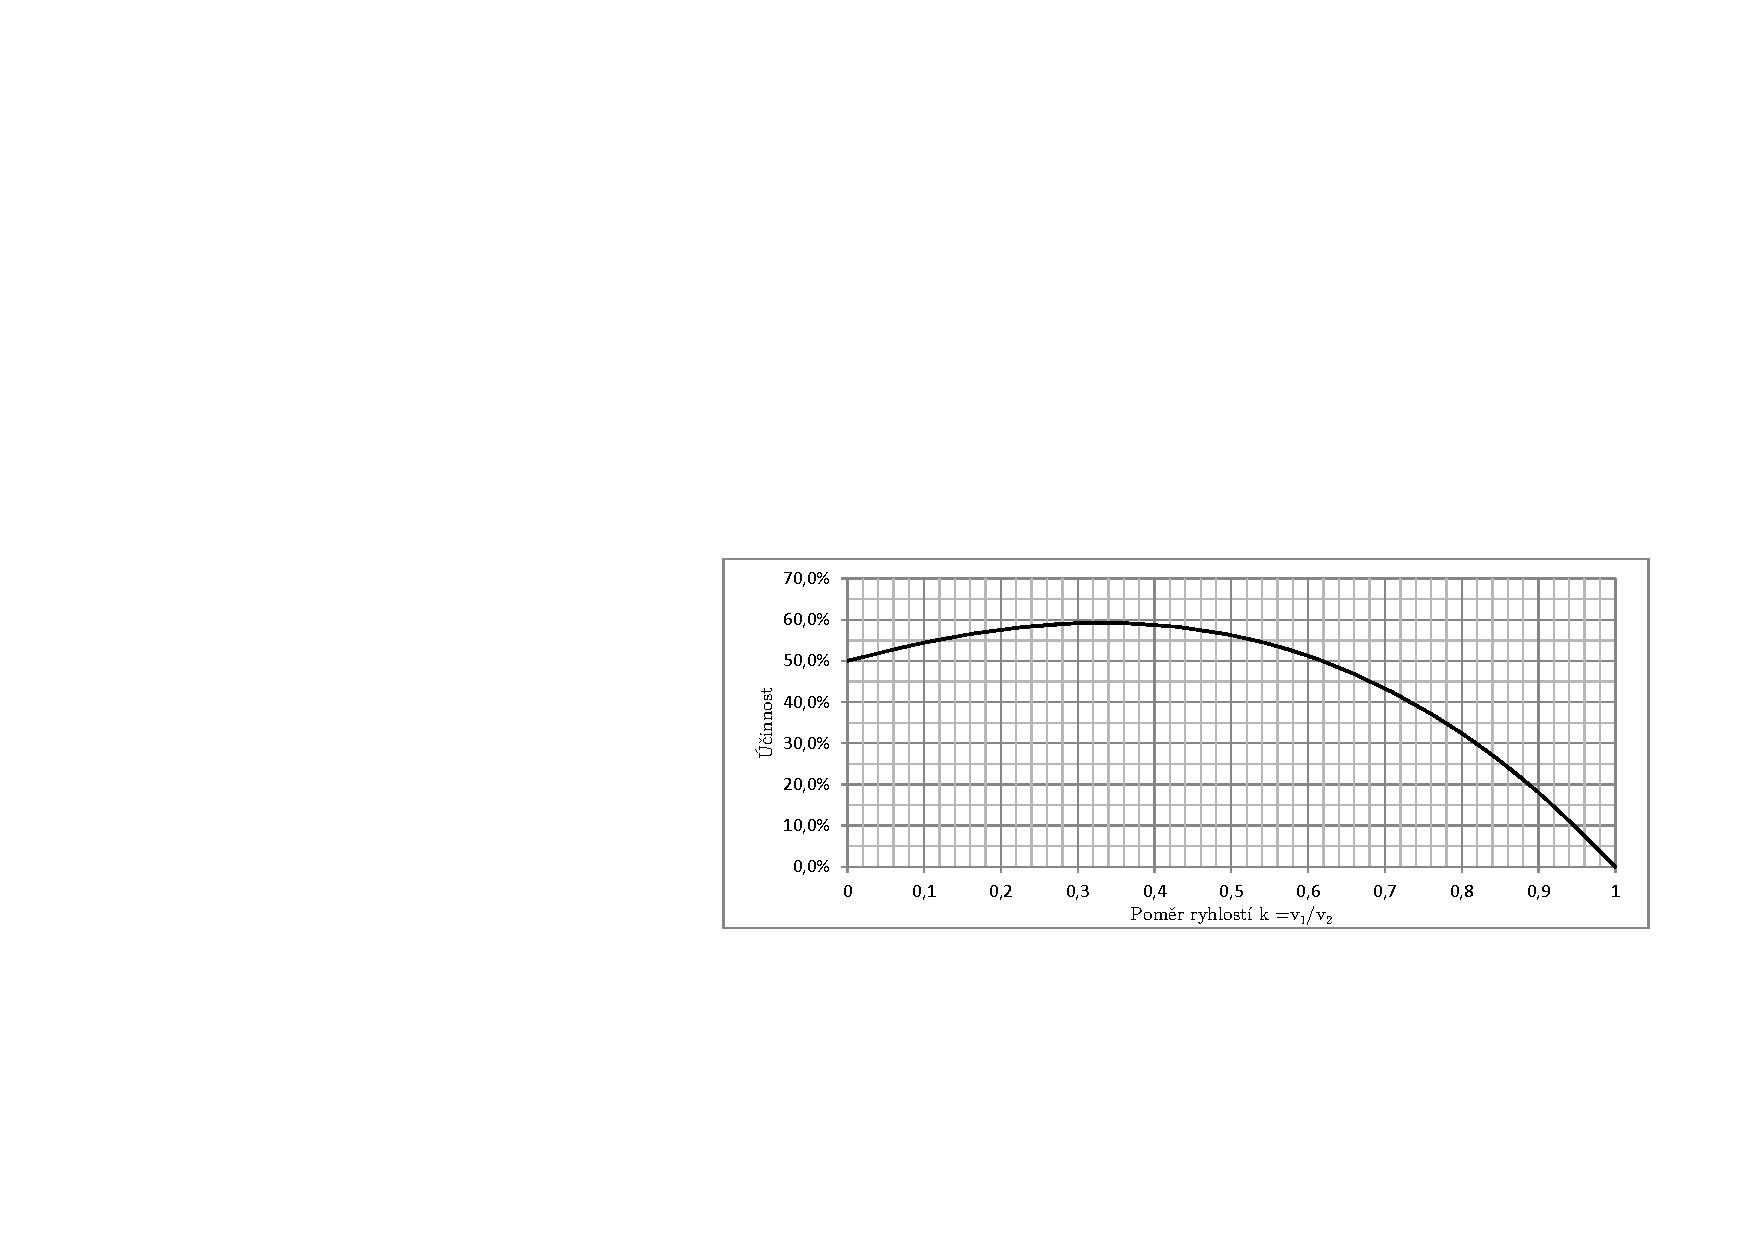
\includegraphics[]{obrazky/grafy/ucinnost}
	          %\input{obrazky/rotor2.ipe}
		\caption{Průběh Betzovy účinnosti pro jednotlivé poměry $v_1/v_2$}
		\label{graf.ucinnost}
	    %\end{center}
	  \end{figure}
	  
	\section {Aerodynamika horizontální vztlakové turbíny}
	V této kapitole shrnuji veškeré důležité teoretické poznatky pro výpočet větrné turbíny. Tyto poznatky jsou poté použity k výpočtu parametrů turbíny v kapitole \ref{chap:praxe}.
	
	Tuto kapitolu jsem rozdělil na tři části. V první části (kapitola \ref{kap:zakladprinc}) jsou vysvětleny základní principy a pojmy ohledně aerodynamických profilů – základního stavebního prvku vztlakových turbín.
	
	Druhá část (kapitola \ref{kap:funkce1}) vysvětluje funkci turbíny a odvozuje základní výpočet. Na tuto kapitolu navazuje kapitola \ref{kap:funkce2}, která tento výpočet rozšiřuje o vírovou teorii.
	
	\subsection{Základní princip, aerodynamický profil}\label{kap:zakladprinc}
	Jak jsem zmínil v předchozích kapitolách, základním principem vztlakových turbín je síla vznikající na rotorovém listu při obtékání vzduchem. Tato síla vzniká díky tvarování listu – podobně jako na křídle letadla. List má v průřezu tvar aerodynamického profilu.
	
	Aerodynamický profil lze nejlépe charakterizovat pomocí obrázku \ref{obr.profil}:
	
	\begin{figure}[H]
		\centering
		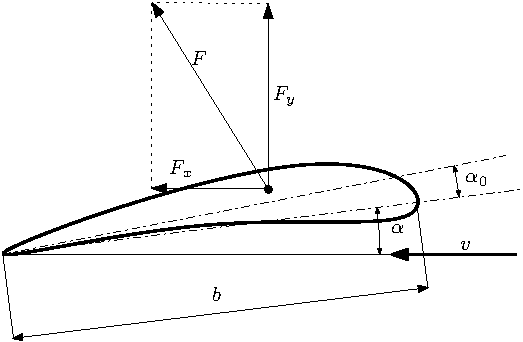
\includegraphics[]{obrazky/profil.pdf}
		\caption{Charakteristika aerodynamického profilu. Inspirováno \cite{Rychetnik:Motory}}
		\label{obr.profil}
	\end{figure}
	
	Profily mají různý tvar; zpravidla jsou však na své náběžné hraně zakulacené a směrem k~odtokové hraně se sbíhají do ostrého konce. Spojnice odtokové hrany s~náběžnou se nazývá tětiva profilu. Zpravidla se značí~$b$. Úhel, který svírá tětiva profilu se směrem pohybu proudu vzduchu (rychlost je zde označena jako $v$), se nazývá úhel náběhu. Běžně se označuje $\alpha$. Často se úhlem $\alpha$ automaticky myslí optimální úhel náběhu, při kterém profil vykazuje nejlepší vlastnosti (poměr sil $F_y$ a $F_x$ je největší). Na obrázku je také vyznačen úhel $\alpha _0$ – úhel nulového vztlaku. Při tomto úhlu náběhu nevzniká na profilu žádná vztlaková síla\cite{Rychetnik:Motory}.
	
	Při obtékání profilu proudem vzduchu vzniká síla $F$. Její velikost a směr jsou závislé na úhlu~$\alpha$. Síla zde vzniká díky vyšší rychlosti obtékajícího vzduchu na vztlakové (na nákresu se jedná o horní stranu) než na podtlakové (spodní) straně. Podle Bernoulliho rovnice klesá v~rychleji se pohybujícím proudu vzduchu statický tlak. Tento podtlak vyvolává vztlakovou sílu\cite{Rychetnik:Motory}.
	
	Pro další úvahy je vhodné rozdělit sílu $F$ na dvě navzájem kolmé složky – $F_x$ a $F_y$. Sílu $F_y$, která je kolmá na směr pohybu proudu vzduchu, nazýváme vztlaková (anglicky označována jako lift force). Sílu $F_x$ nazýváme odporovou (anglicky drag force). Tato síla působí proti směru pohybu profilu a je nežádoucí – snižuje účinnost rotoru\cite{Rychetnik:Motory}\cite{ve:ve}.
	
	Velikost těchto sil je možno spočítat pomocí součinitele vztlaku $c_y$ (v anglické literatuře označován jako $c_L$ – lift coefficient) a součinitele odporu $c_x$ (ang. $c_d$, drag coefficient). Tyto součinitelé jsou vždy platní pouze pro určitý úhel náběhu a Reynoldsovo číslo (viz dále). Dají se zjistit experimentálně, případně pomocí CFD simulace. Na základě těchto součinitelů lze síly $F_x$ a $F_y$ spočítat následovně \eqref{rov:11}\cite{Rychetnik:Motory}:
	
	\begin{eqnarray}
			\label{rov:11}
			F_x \frac{1}{2}\rho c_x Sv^2 \nonumber \\
			F_y \frac{1}{2}\rho c_y Sv^2
	\end{eqnarray}
	Kde $\rho$ označuje hustotu vzduchu, $v$ rychlost proudu vzduchu a $S$ plochu listu. V dalších kapitolách bude často uvažována nekonečně malá část rotorového listu a za $S$ se bude dosazovat $dS$, které lze definovat následovně\eqref{rov:12}\cite{Rychetnik:Motory}: 
	
		\begin{equation}
				\label{rov:12}
				S=b\;\mathrm{d}r
		\end{equation}
	Kde $\mathrm{d}r$ je nekonečně malá vzdálenost mezi 2 poloměry $r_1$ a $r_2$ na rotorovém listu a $b$ je délka tětivy.
	
	Na grafech \ref{graf:zavislost1} a \ref{graf:zavislost2} je znázorněn průběh součinitelů vztlaku a odporu v závislosti na úhlu náběhu pro profil SG6043 (při Reynoldsově čísle $10^5$).
	
	\begin{figure}[H]
	\centering
	\subfigure[Závislost součinitele vztlaku na úhlu náběhu. ]{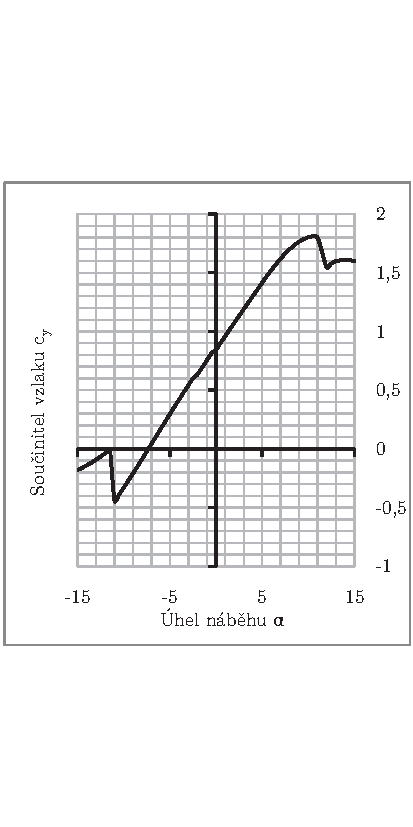
\includegraphics[]{obrazky/grafy/odvozeni3p}\label{graf:zavislost1}}~
	\subfigure[Závislost součinitele odporu na úhlu náběhu. ]{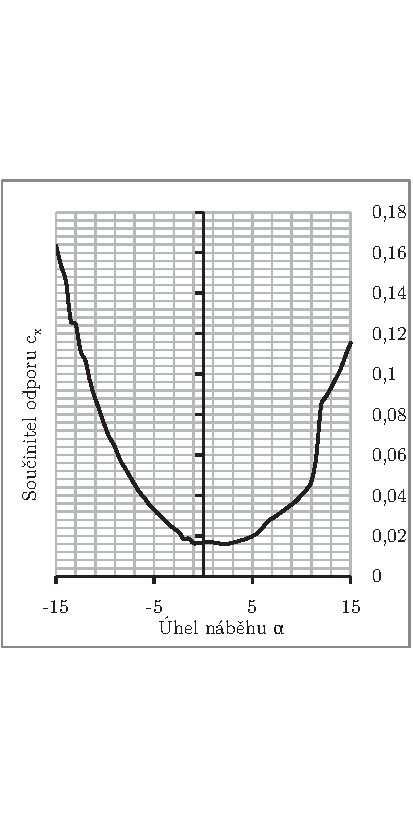
\includegraphics[]{obrazky/grafy/odvozeni2p}\label{graf:zavislost2}}
	\caption{Závislosti součinitelů $c_x$ a $c_y$ u profilu SG6043 při $Re=10^5$. Data převzata z \cite{profil}}
	\end{figure}
	
	Jak jsem zmínil výše, aerodynamické vlastnosti profilu nejsou vždy stejné. Pro charakteristiku podmínek, při kterých byly naměřeny dané hodnoty, se používá Reynoldsovo číslo $Re$. Jedná se o bezrozměrnou veličinu popisující proudění. Reynoldsovo číslo je definováno následovně\eqref{rov:13}\cite{Rychetnik:Motory}:
	\begin{equation}
					\label{rov:13}
					Re=\frac{vl}{\nu}
	\end{equation}
	Kde ve vztahu \eqref{rov:13} $v$ je rychlost obtékání profilu, $l$ je délka tětivy a $\nu$ je kinematická viskozita vzduchu.
	
	Reynoldsovo číslo se pohybuje pro malé rotory (do 10~m) v rozmezí $10^5$–$10^7$\cite{ve:ve}. Ze vzorce je patrné, že Reynoldsvo číslo je pouze orientační údaj – ve vzorci vystupuje rychlost obtékání a~délka tětivy. Obě tyto veličiny se u listů větrné turbíny mění v závislosti na vzdálenosti od osy otáčení. Proto se také často počítá se zaokrouhlenou hodnotou kinematické viskozity vzduchu $1,5\cdot 10^{-6}\;m\cdot s^{-2}$\cite{Rychetnik:Motory}.
	
	\subsection{Funkce horizontální vztalkové turbíny}\label{kap:funkce1}
	Cílem této kapitoly je objasnit, jaký tvar (úhel náběhu a délku tětivy) by rotorový list měl mít, aby dosahoval co nejlepších vlastností.
	
	Na otáčející se turbíně se nachází rotorový list v~situaci na obrázku \ref{obr.profilprostor}).
	
	\begin{figure}[H]
		\centering
		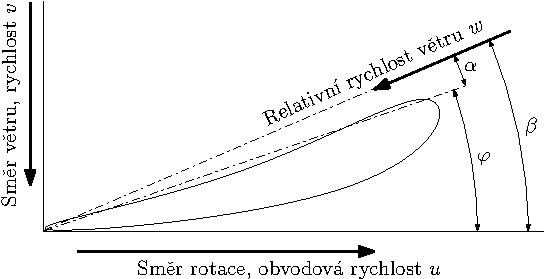
\includegraphics[]{obrazky/profilnavrtuli}
		\caption{Rotorový list na otáčející se turbíně. Inspirováno \cite{Rychetnik:Motory}.}
		\label{obr.profilprostor}
	\end{figure}
	Obrázek \ref{obr.profilprostor} zobrazuje část (řez) rotorového listu na poloměru $r$. Celý list se otáčí úhlovou rychlostí $\omega$, prvek na poloměru $r$ má pak tedy obvodovou rychlost $u$ \eqref{rov:14}\cite{Rychetnik:Motory}:
	\begin{equation}
		\label{rov:14}
		u=\omega r=\frac{\pi n}{30}r
	\end{equation}
	Kde $n$ jsou otáčky za minutu, které jsou zde uvedeny, jelikož jsou pro představu názornější než úhlová rychlost. Rovnoběžně s~osou otáčení fouká vítr rychlostí $v$. Je důležité si všimnout orientace profilu listu – tlaková strana je nastavena proti směru větru. Je tedy opačně orientován než u běžných leteckých vrtulí. U leteckých vrtulí má list opačnou funkci – místo zpomalování proud vzduchu jej urychluje.
	
	Vektorovým součtem obvodové rychlosti $u$ a rychlosti větru $v$ získáváme relativní rychlost větru $w$. Platí tedy \eqref{rov:15}\cite{Rychetnik:Motory}.
	\begin{equation}
		\label{rov:15}
		w=\sqrt{u^2 + v^2}
	\end{equation}
	Rychlostí $w$ (a v jejím směru) je rotorový list ofukován. Na obrázku je vyznačen úhel $\beta$, který rychlost $w$ svírá s~osou otáčení. Z~obrázku je tedy patrný vztah \eqref{rov:16}\cite{Rychetnik:Motory}:
	\begin{equation}
		\label{rov:16}
		\tan{\beta}=\frac{v}{u}
	\end{equation}
	Z rovnice \eqref{rov:16} vyplývá důležitý poznatek – jelikož je rychlost v konstantní a obvodová rychlost u závisí na poloměru $r$, nemá rotorový list po celé své délce stejný úhel náběhu. Obdobně se dá předpokládat, že ani délka tětivy $b$ nebude po celé délce listu konstantní. Proto musí být veškeré úvahy prováděny na (nekonečně) malém úseku mezi poloměrem $r$ a $r + \mathrm{d}r$.
	
	Úhel $\alpha$, který svírá tětiva profilu s~relativní rychlostí proudu vzduchu, zde značí optimální úhel náběhu – poměr součinitelů $c_y/c_x$ je největší možný pro daný profil.
	
	Na rotorovém listu při obtékání vzduchem vzniká vztlaková síla. Tu můžeme rozložit podle obrázku \ref{obr.profilsil}.
	\begin{figure}[h]
		\centering
		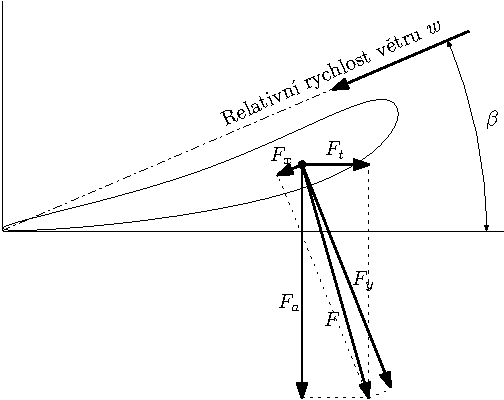
\includegraphics[]{obrazky/sily}
		\caption{Rozklad sil na rotorovém listu. Inspirováno \cite{Rychetnik:Motory}.}
		\label{obr.profilsil}
	\end{figure}
	Síly $F_x$ a $F_y$ lze spočítat z rovnice \ref{rov:11}. Jejich výslednice lze rozložit na 2 složky – sílu $F_t$, která otáčí rotorem, a sílu $F_a$, která působí na stožár a na užitečném výkonu turbíny se nepodílí. Síla $F_t$, respektive její element $\mathrm{d}F_t$ na prvku $r$, vyvolává elementární moment síly dle \eqref{rov:17}\cite{Rychetnik:Motory}.
	\begin{equation}
		\label{rov:17}
		\mathrm{d}M=\mathrm{d}F_t r
	\end{equation}
	Jelikož se v dalších výrazech vyskytuje úhel $\beta$, je vhodné vyjádřit $w$ také pomocí úhlu $\beta$ \eqref{rov:18}\cite{Rychetnik:Motory}:
	\begin{eqnarray}
				\label{rov:18}
			u=v \cot\beta \nonumber \\
			w^2 = 1 + cotg^2 \beta
	\end{eqnarray}
	Poté lze vyjádřit sílu v axiálním směru ve tvaru \eqref{rov:19}\cite{Rychetnik:Motory}.
	\begin{equation}
		\label{rov:19}
		\mathrm{d}F_a=\frac{1}{2}v^2\rho\;\mathrm{d}S(1+cotg^2 \beta)(c_y \cos \beta + c_x \sin \beta)
	\end{equation}
	Kde $(c_y \cos\beta+c_x \sin \beta)$ vychází z obrázku \ref{obr.odvozeni1}.
	\begin{figure}[H]
		\centering
		\subfigure[Zde lze vidět, že síla $F_a$ je složena z~přilehlé odvěsny přepony velkého trojúhelníku s~úhlem $\beta$ a protihlehlé odvěsny malého trojúhelníku s~úhlem~$\beta$ ]{
\includegraphics[]{obrazky/odvozeniplusp}\label{obr.odvozeni1}}~
		\subfigure[Zde lze vidět, že síla $F_t$ je rovna protilehlé odvěsně velkého trujúhelníku s~úhlem $\beta$ mínus přilehlá odvěsna malého trojúhelníku s~úhlem~$\beta$]{
\includegraphics[]{obrazky/odvozeniminusp}\label{obr.odvozeni2}}
		\caption{Odvození vztahů pro síly na profilu}
	\end{figure}
	Obdobně lze vyjádřit i element síly $F_t$ \eqref{rov:20}\cite{Rychetnik:Motory}.
	\begin{equation}
			\label{rov:20}
			\mathrm{d}F_t=\frac{1}{2}v^2\rho\;\mathrm{d}S(1+cotg^2 \beta)(c_y \sin \beta - c_x \cos \beta)
	\end{equation}
	V knize \cite{Rychetnik:Motory} se ve výrazu \eqref{rov:20} nachází chyba (překlep), kdy je v poslední závorce znaménko plus místo mínus. Důkaz znaménka mínus vyplývá z obrázku \ref{obr.odvozeni2}.
	
	Z výše vyjádřené síly $F_t$ lze určit elementární moment a elementární užitečný výkon vznikající na daném prvku rotoru \eqref{rov:21}\cite{Rychetnik:Motory}.
	\begin{eqnarray}
		\label{rov:21}
		\mathrm{d}M=\frac{1}{2}v^2\rho \; \mathrm{d}Sr(1+cotg^2 \beta) (c_y\sin\beta - c_x\cos \beta)\nonumber \\
		\mathrm{d}P_u=\mathrm{d}M\omega=\mathrm{d}M\frac{u}{r}=\mathrm{d}M\frac{v \cot\beta}{r}\nonumber \\
		\mathrm{d}P_u=\frac{1}{2}v^3\rho\;\mathrm{d}S(1+cotg^2 \beta)(c_y\sin \beta-c_x\cos\beta)\cot\beta
	\end{eqnarray}
	Tímto byly shrnuty veškeré základní poznatky, které je nutno o vztlakové horizontální turbíně vědět. Zbývá už jen z~těchto poznatků vyjádřit, jak má co nejideálnější turbína vypadat.
	
	Základním parametrem větrné turbíny je již dříve zmíněná rychloběžnost. Zpravidla se značí~$\lambda$ (někdy se lze setkat i s~označením $\lambda_0$). Jedná se o bezrozměrnou veličinu, která popisuje poměr obvodové rychlosti turbíny $u_R$ vůči rychlosti větru před turbínou $v_1$\eqref{rov:22}\cite{Rychetnik:Motory}.
	\begin{equation}
			\label{rov:22}
			\lambda = \frac{u_R}{v_1}
	\end{equation}
	Tento parametr turbíny se zpravidla volí (odvisí od něj otáčky rotoru), je však omezen daným typem turbíny. Například rotor Savonius je schopný efektivně pracovat při rychloběžnosti 0,85–1,8, \uv{americké kolo} 1,1–2, třílistá horizontální turbína 2–6, dvoulistá 6–10. Třílistý rotor Darrieus 4,6–6,8 a jednolistý 6–10. Tyto údaje byly převzaty z~\cite{Rychetnik:Motory} a~\cite{ve:ve}. Z~předchozích poznatků vyplývá, že ideální rotor má konstantní rychloběžnost a tudíž je neregulovatelný. Jakoukoliv regulaci otáček je možné provést pouze za cenu snížení účinnosti.
	
	Můžeme také definovat rychloběžnost pro prvek na listu ve vzdálenosti $r$ od středu \eqref{rov:23}\cite{Rychetnik:Motory}.
	\begin{equation}
		\label{rov:23}
		\lambda_r = \frac{u_r}{v_1}=\frac{r}{R}\lambda
	\end{equation}
	V kapitole \ref{ucinnost} vyplynulo z Betzovi účinnosti, že rotor má maximální účinnost právě tehdy, platí-li \eqref{rov:24}.	
	\begin{equation}
			\label{rov:24}
			v_2 = \frac{1}{3}v_1
	\end{equation}
	Z rovnice \eqref{rov:5} v kapitole \ref{ucinnost} vyplývá, že rychlost v rovině rotoru $v$ je rovna \eqref{rov:25}\cite{Rychetnik:Motory}.
	\begin{equation}
		\label{rov:25}
		v = \frac{v_1+v_2}{2}=\frac{v_1+\frac{1}{3}v_1}{2}=\frac{2}{3}v_1
	\end{equation}
	Díky vyjádření z~rovnice \eqref{rov:25} lze dosazením do rovnice \eqref{rov:16} spočítat~$\beta$ pro jednotlivé prvky listu ve vzdálenosti~$r$ od středu rotoru\eqref{rov:26} – tedy jednu ze dvou charakteristik tvaru listu (druhou je délka tětivy)\cite{Rychetnik:Motory}.
	\begin{eqnarray}
		\label{rov:26}
		\tan\beta=\frac{v}{u_r}=\frac{\frac{2}{3}v_1}{\lambda_r v_1}=\frac{2}{\frac{3r\lambda}{R}} \nonumber \\
		\beta = \arctan(\frac{2R}{3r\lambda})
	\end{eqnarray}
	K tomuto vyjádření je nutné připomenout obrázek \ref{obr.profilprostor}. Z~něj je patrné, že úhel $\beta$ není odchylkou tětivy profilu od roviny rotoru. Odchylku tětivy profily je úhel $\varphi$, který lze určit dle \eqref{rov:27}.
	\begin{equation}
		\label{rov:27}
		\varphi = \beta - \alpha
	\end{equation}
	Kde $\alpha$ je optimální úhel náběhu daného aerodynamického profilu.
	
	Délku tětivy lze spočítat z předpokladu, který vyplývá z Betzovy účinnosti – proud vzduchu musí být turbínou zpomalen na $\frac{1}{3}$  své původní rychlosti. Proud vzduchu vyvolává na rotoru axiální sílu. Axiální sílu působící na jeden element rotoru lze změnou hybnosti vyjádřit dle \eqref{rov:28}\cite{Rychetnik:Motory}.
	\begin{eqnarray}
		\label{rov:28}
		\mathrm{d}F_a=\rho\; \mathrm{d}V(v_1 - v_2) \nonumber \\
		\mathrm{d}V=2\pi r \; \mathrm{d}r\frac{v_1+v_2}{2} \nonumber \\
		\mathrm{d}F_a=2\pi\rho r\; \mathrm{d}r\frac{v_1+v_2}{2}(v_1-v_2)
	\end{eqnarray}
	Axiální sílu lze však vyjádřit i pomocí aerodynamických sil (jak je popsáno v rovnici \eqref{rov:19}). Kniha \cite{Rychetnik:Motory} tento výpočet dle mě zbytečně zjednodušuje – zanedbává vliv odporové síly vznikající na profilu listu. Já jej však budu nadále uvažovat. Rovnice \eqref{rov:19} však představuje sílu působící pouze na jeden list; celková síla axiální síla je \eqref{rov:29}:
	\begin{equation}
			\label{rov:29}
			\mathrm{d}F_a=\frac{1}{2}v^2z\rho\;\mathrm{d}S(1+cotg^2 \beta)(c_y \cos \beta + c_x \sin \beta)
	\end{equation}
	Kde $z$ je počet listů rotoru.
	
	Porovnáním dvou vyjádření axiální síly a dosazením vztahů \eqref{rov:28} a \eqref{rov:29} lze získat vztah \eqref{rov:30} vyjadřující délku tětivy $b$ pro element listu na poloměru $r$.
	
	\begin{eqnarray}
		\label{rov:30}
		2\pi\rho r\; \mathrm{d}r\frac{v_1+v_2}{2}(v_1-v_2)=\frac{1}{2}\left( \frac{v_1 + v_2}{2} \right)^{2} z\rho b\;\mathrm{d}r(1+cotg^2 \beta)(c_y \cos \beta + c_x \sin \beta) \nonumber \\
		2\pi r(v_1-v_2)=\frac{1}{2} zb(1+cotg^2 \beta)(c_y \cos \beta + c_x \sin \beta)\left( \frac{v_1 + v_2}{2} \right) \nonumber \\
		2\pi r\frac{2}{3}v_1=\frac{1}{2} zb(1+cotg^2 \beta)(c_y \cos \beta + c_x \sin \beta )\frac{2}{3}v_1 \nonumber \\
		b=\frac{4\pi r}{z(1+cotg^2 \beta)(c_y \cos \beta + c_x \sin \beta )}
	\end{eqnarray}
	Toto vyjádření není v ideální podobě (bylo by vhodné ještě vyjádřit funkce úhlu $\beta$ pomocí poloměru a rychloběžnosti), ale i přesto poskytuje jasnou představu o délce tětivy na listu.
	
	Na grafech \ref{graf.delka1} a \ref{graf.nabeh1} lze najít průběh délky tětivy a úhlu odchylky tětivy od rotoru na prvním prototypu větrné turbíny. Je zde zahrnuto i porovnání výpočtu uvažujícího odporovou sílu a výpočtu, který ji neuvažuje.
	
	\begin{figure}[H]
			%\begin{center}
			\centering
				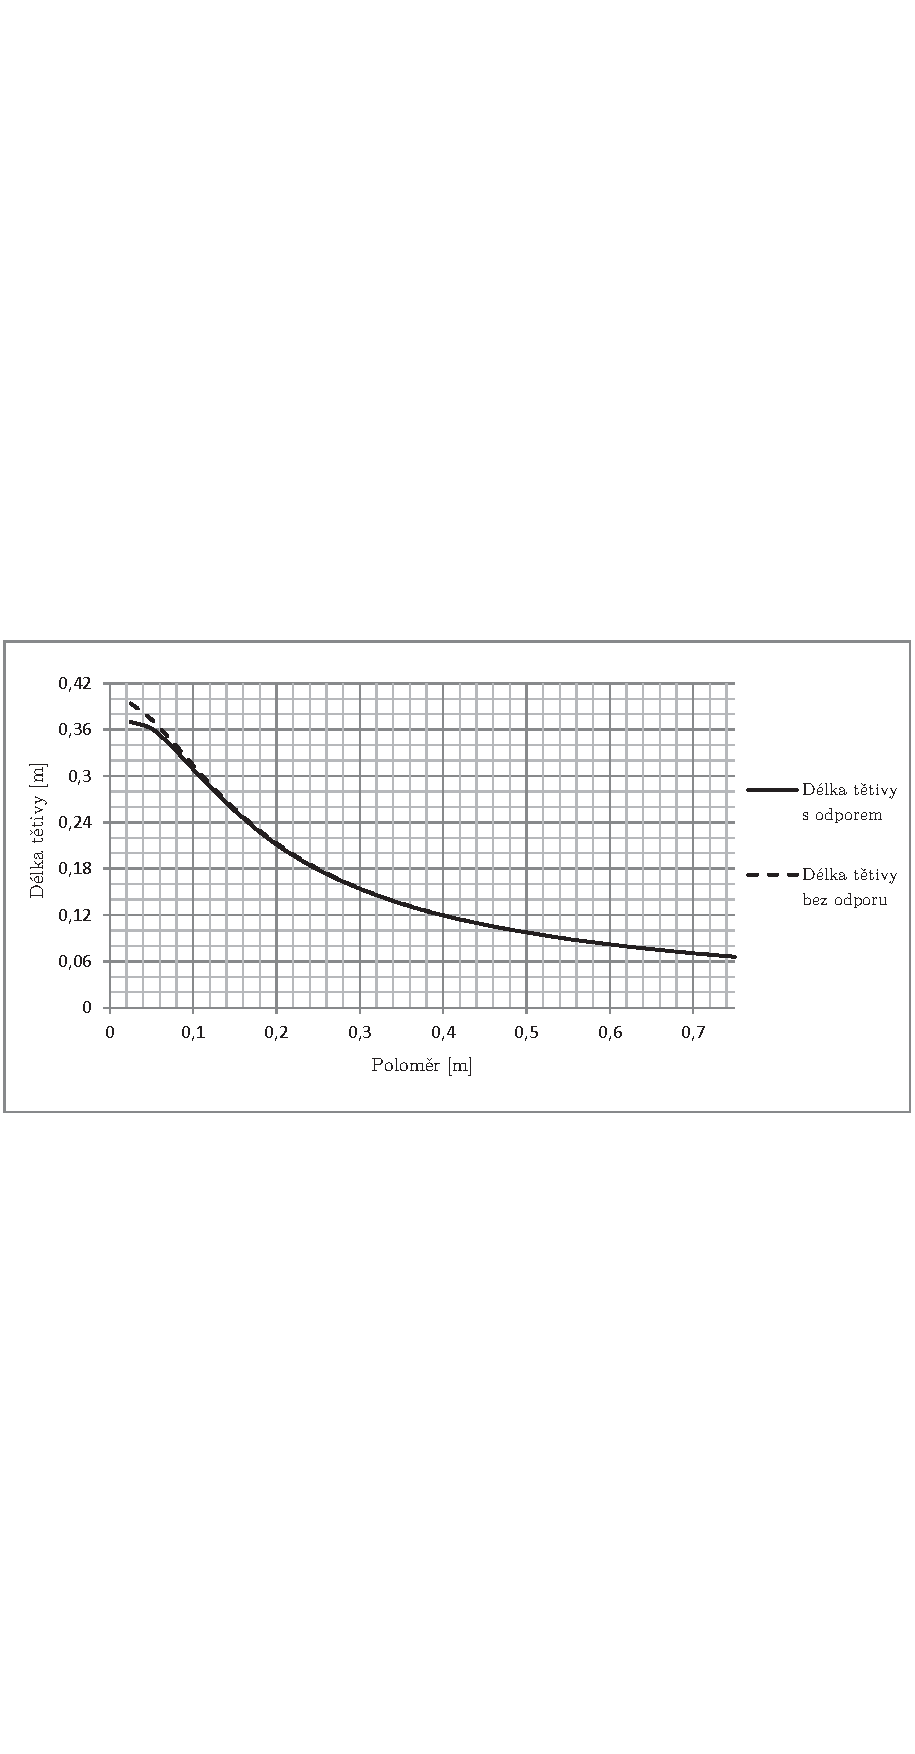
\includegraphics[]{obrazky/grafy/delkap}
		          %\input{obrazky/rotor2.ipe}
			\caption{Délka tětivy prvního prototypu trubíny. Turbína má tři listy, rychloběžnost 4, a poloměr 75~cm. Používá profil SG6043 s $c_x$ 1,303 a $c_y$ 0,017. Je zde patrný minimální rozdíl mezi výpočtem s~odporem a bez odporu.}
			\label{graf.delka1}
		    %\end{center}
		  \end{figure}
		  
	\begin{figure}[H]
				%\begin{center}
				\centering
					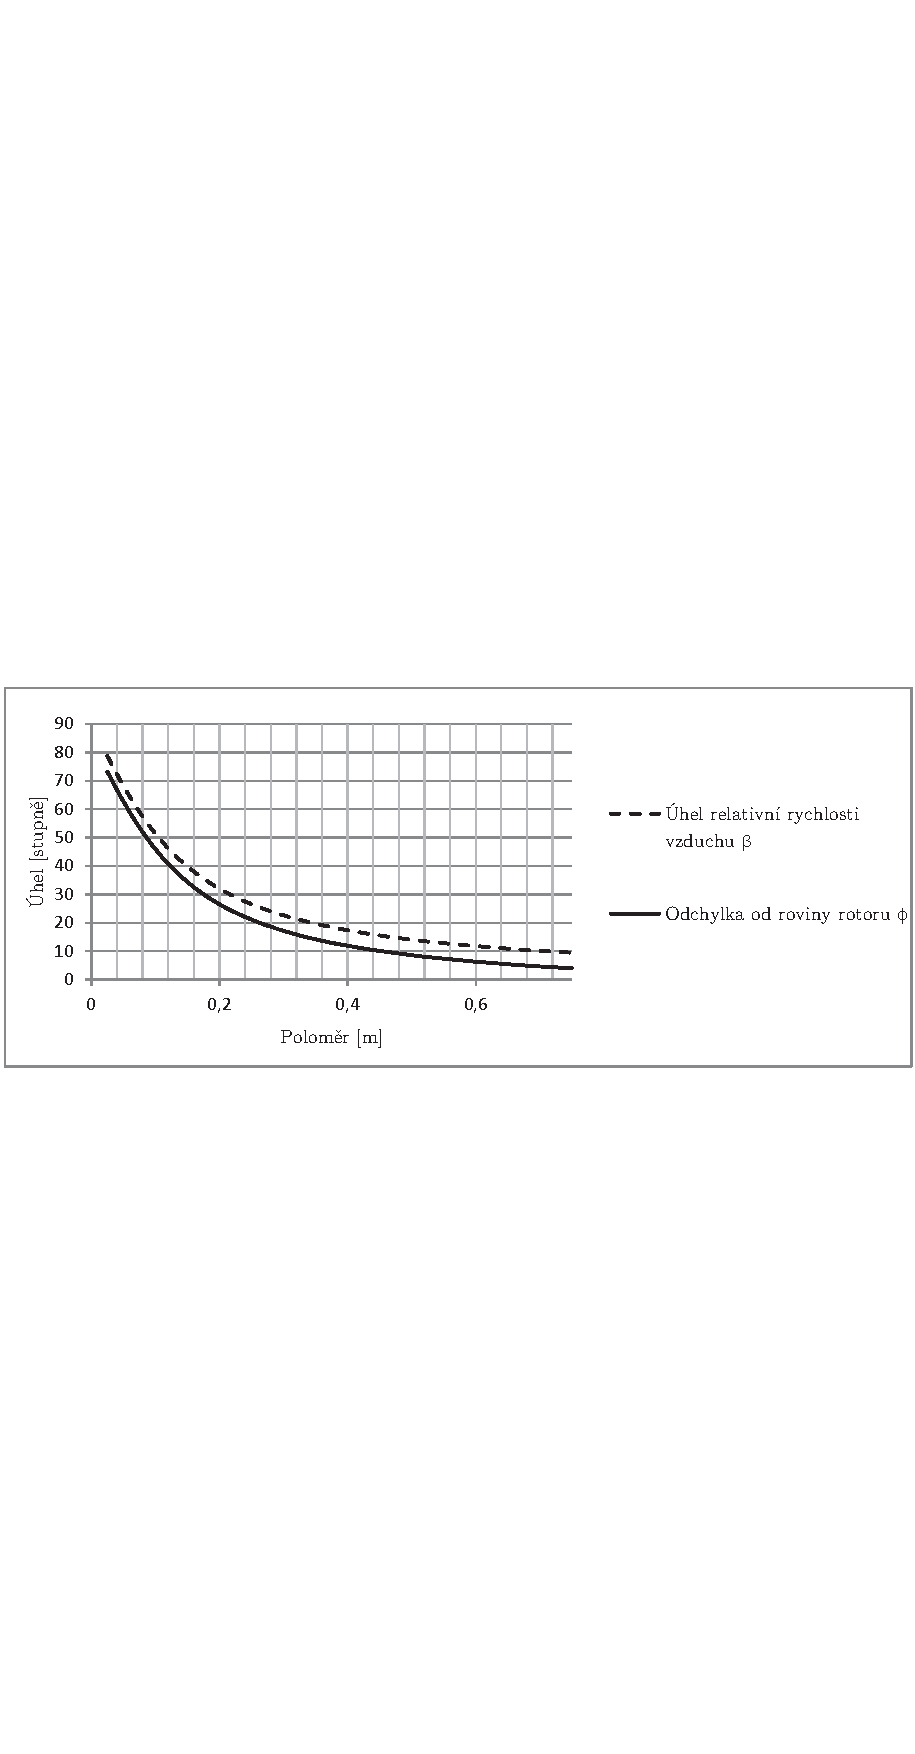
\includegraphics[]{obrazky/grafy/nabehp}
			          %\input{obrazky/rotor2.ipe}
				\caption{Graf znázorňující průběh odchylky tětivy od roviny rotoru a úhel relativní rychlosti vzduchu. Je zde uvažován ideální úhel náběhu profilu SG6043 $5,5\,^{\circ}$.}
				\label{graf.nabeh1}
			    %\end{center}
	\end{figure}
	
	
	\subsection{Rozšířený výpočet, vírová teorie}\label{kap:funkce2}
	
	Výpočet tvaru listu v předchozí kapitole má jeden nedostatek – předpokládá, že turbína proudu za rovinou rotoru neuděluje žádnou rotační složku. Avšak této vlastnosti může dosáhnout pouze ideální turbína, jejíž lopatky jsou nekonečně tenké a nevznikají na nich žádné třecí síly.
	
	Teorii uvažující vír vznikající za rotorem poprvé popsal britský aerodynamik Hermann Glauert. V této kapitole tuto teorii popisuji. Na konci této kapitoly uvádím porovnání výsledků výpočtů zjednodušené a Glauertovy teorie.
	
	Glauertova vírová teorie předpokládá, že proud vzduchu před rotorem má nulovou rotační složku (úhlová rychlost je nulová). Po průchodu rotorem bude proudu vzduchu udělena úhlová rychlost $\Omega$. Stejně jako v předchozí teorii, platí, že rychlost $v$~v rovině rotoru je aritmetickým průměrem rychlosti před rotorem $v_1$ a rychlosti za rotorem     $v_2$. Obdobně je i úhlová rychlost proudu v rovině aritmetickým průměrem rychlosti před rotorem a za ním; tedy $\frac{\Omega}{2}$\cite{Rychetnik:Motory}.
	
	Pro další úvahy je vhodné vyjádřit přírůstek úhlové rychlosti proudu vzduchu k~úhlové rychlosti rotoru $\omega$ pomocí koeficientu $h$ a poměr rychlostí před a za rotorem pomocí koeficientu~$k$.
	
	Jelikož má tento vír opačný směr otáčení než rotor, platí výraz \eqref{rov:31}\cite{Rychetnik:Motory}.
	
		\begin{eqnarray}
			\label{rov:31}
			\omega + \Omega = h\omega \nonumber \\
			\Omega = (h-1)\omega
		\end{eqnarray}
	Obdobně lze vyjádřit poměr rychlostí $v_1$ a $v_2$ \eqref{rov:32}\cite{Rychetnik:Motory}.
	\begin{eqnarray}
				\label{rov:32}
				k = \frac{v_2}{v_1} \nonumber \\
				v_2 = kv_1
	\end{eqnarray}
	Úhlovou rychlost proudu v rovině rotoru lze pomocí koeficientu vyjádřit následovně \eqref{rov:33}\cite{Rychetnik:Motory}:
	\begin{equation}
		\label{rov:33}
		\omega + \frac{\Omega}{2}=\frac{1+h}{2}\omega
	\end{equation}
	Stejně tak rychlost proudu vzduchu v rovině rotoru $v$ lze vyjádřit pomocí koeficientu $k$ - vztah \eqref{rov:34}\cite{Rychetnik:Motory}:
	\begin{equation}
			\label{rov:34}
			v =\frac{v_1 + v_2}{2}=\frac{1+k}{2}v_1
	\end{equation}
	Dalším cílem je pomocí nově definovaných rychlostí určit úhel relativní rychlosti proudu vzduchu $\beta$. Jeho určení je podobné jako ve zjednodušené teorii – vychází z obrázku \ref{obr.profilprostor}.
	Pro vyjádření úhlu $\beta$ je zapotřebí znát obvodovou rychlost prvku na rotoru ve vzdálenosti $r$ od osy otáčení \eqref{rov:35}\cite{Rychetnik:Motory}.
	\begin{equation}
		\label{rov:35}
		u =\frac{1+h}{2}\omega r
		\end{equation}
	Úhel $\beta$, který svírá směr relativní rychlosti proudu vzduchu $w$ s rovinou rotoru, lze potom vyjádřit následovně \eqref{rov:36}\cite{Rychetnik:Motory}:
	\begin{equation}
			\label{rov:36}
			\cot \beta = \frac{u}{v}=\frac{\frac{1+h}{2}\omega r}{\frac{1+k}{2}v_1}=\frac{1+h}{1+k}\lambda_r
	\end{equation}
	Velikost rychlosti $w$ je z~obrázku \ref{obr.profilprostor} rovna\eqref{rov:37}\cite{Rychetnik:Motory}:
	\begin{equation}
		\label{rov:37}
		w=\frac{v_1 (1+k)}{2\sin\beta}=\frac{\omega r(1+h)}{2\cos\beta}
	\end{equation}
	Další kroky jsou v podstatě stejné jako u zjednodušené teorie – je tedy nutné vyjádřit jednotlivé síly působící na elementy rotorového listu pomocí základní aerodynamiky vzduchového proudu a aerodynamických vlastností profilu listu. Pouze se zde dosazují výše odvozené rychlosti.
	
	Tudíž z výše uvedených vztahů lze sestavit rovnici pro axiální sílu $F_a$ - vztah \eqref{rov:38}\cite{Rychetnik:Motory}:
	\begin{equation}
		\label{rov:38}
	\mathrm{d}F_a = \mathrm{d}F_y\cos\beta+\mathrm{d}F_x\sin\beta = \frac{1}{2}\rho bw^2\; \mathrm{d}r(c_y\cos\beta + c_x\sin\beta)
	\end{equation}
	Obdobně lze také sestavit výraz pro tangenciální sílu $F_t$ \eqref{rov:39}. V~knize \cite{Rychetnik:Motory} je opět zaměněno znaménko.
	\begin{equation}
			\label{rov:39}
		\mathrm{d}F_t = \mathrm{d}F_y\sin\beta-\mathrm{d}F_x\cos\beta = \frac{1}{2}\rho bw^2\; \mathrm{d}r(c_y\sin\beta - c_x\cos\beta)
		\end{equation}
	Jelikož se zde objevují výrazy s~goniometrickými funkcemi, je výhodné převést vyjádření součinitelů vztlaku a odporu na goniometrický tvar. Celý převod vychází z obrázku \ref{obr.epsilon}.
	\begin{figure}[H]
					\centering
						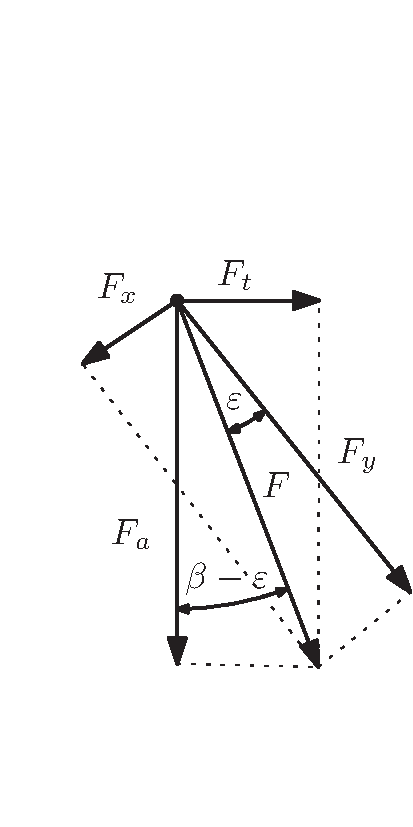
\includegraphics[]{obrazky/odvozeniepsilonp}
					\caption{Obrázek znázorňuje vyjádření sil $F_a$ a $F_t$ pomocí úhlu $\varepsilon$}
					\label{obr.epsilon}
				    %\end{center}
	\end{figure}
	Z obrázku \ref{obr.epsilon} vyplývá výraz \eqref{rov:40}\cite{Rychetnik:Motory}.
	\begin{equation}
		\label{rov:40}
		\tan \varepsilon = \frac{F_x}{F_y} = \frac{c_x}{c_y}
	\end{equation}
	Poté lze vyjádřit sílu $F_a$ následovně \eqref{rov:41}\cite{Rychetnik:Motory}:
	\begin{eqnarray}
		\label{rov:41}
		\cos \varepsilon = \frac{F_y}{F}\Rightarrow F=\frac{F_y}{\cos \varepsilon} \nonumber \\
		F_a = F\cos(\beta-\varepsilon)=\frac{F_y}{\cos\varepsilon}\cos(\beta-\varepsilon) \nonumber \\
		\mathrm{d}F_a=\frac{1}{2}\rho bw^2\;\mathrm{d}r\frac{c_y}{\cos\varepsilon}\cos(\beta - \varepsilon)
	\end{eqnarray}
	Obdobně lze vyjádřit i sílu Ft\eqref{rov:42}\cite{Rychetnik:Motory} a celkovou axiální sílu působící na všechny listy rotoru\eqref{rov:43}\cite{Rychetnik:Motory}.
	\begin{equation}
		\label{rov:42}
		\mathrm{d}F_t=\frac{1}{2}\rho bw^2\;\mathrm{d}r\frac{c_x}{\cos\varepsilon}\sin(\beta - \varepsilon)
	\end{equation}
	\begin{equation}
		\label{rov:43}
		\mathrm{d}F_{az}=\frac{1}{2}z\rho bw^2\;\mathrm{d}r\frac{c_y}{\cos\varepsilon}\cos(\beta - \varepsilon)
	\end{equation}
	Pomocí síly $F_t$ lze vyjádřit i celkový moment síly působící na všechny listy rotoru\eqref{rov:44}\cite{Rychetnik:Motory}.
	\begin{equation}
			\label{rov:44}
			\mathrm{d}M=rz\;\mathrm{d}F_t=\frac{1}{2}rz\rho bw^2\;\mathrm{d}r\frac{c_x}{\cos\varepsilon}\sin(\beta - \varepsilon)
		\end{equation}
	Axiální sílu na rotor lze stejně jako v odvození Betzovy účinnosti pomocí změny hybnosti proudu vzduchu. Proud vzduchu v~prstenci mezi poloměry $r$ a $r + \mathrm{d}r$ působí silou $\mathrm{d}F_a$ vyjádřené dle \eqref{rov:45}\cite{Rychetnik:Motory}.
	\begin{eqnarray}
		\label{rov:45}
		\mathrm{d}F_a\Delta t=m(v_1-v_2) \nonumber \\
		m=2\pi\rho r\;\mathrm{d}rv=\pi\rho r\;\mathrm{d}r(1+k)v_1 \nonumber \\
		\mathrm{d}F_a=\pi\rho r\;\mathrm{d}r(1+k)v_1\Delta v = \pi\rho r\;\mathrm{d}r(1-k^2)v_1^2
	\end{eqnarray}
	Moment síly na element rotoru mezi poloměry $r$ a $r + \mathrm{d}r$ lze také určit i ze změny momentu hybnosti proudu\eqref{rov:46}\cite{Rychetnik:Motory}. Jelikož je úhlová rychlost proudu před rotorem nulová, je změna úhlové rychlosti rovna $\Omega$.
	\begin{eqnarray}
		\label{rov:46}
		\mathrm{d}M = mru = mr^2\Omega \nonumber \\
		\mathrm{d}M=\rho\pi r^3\; \mathrm{d}r v_1(1+k)\Omega = \rho\pi r^3\; \mathrm{d}r v_1\omega(1+k)(h-1)
		\end{eqnarray}
		Další krok je podobný jako ve zjednodušené teorii – je nutné stejné, ale jinak vyjádřené, veličiny porovnat. Porovnáním axiální síly z rovnic \eqref{rov:43} a \eqref{rov:45} a dosazením relativní rychlosti proudu vzduchu $w$ z~rovnice \eqref{rov:37} dostaneme \eqref{rov:47}\cite{Rychetnik:Motory}.
		\begin{eqnarray}
			\label{rov:47}
			\frac{1}{2}\rho bzw^2\;\mathrm{d}r\frac{c_y}{\cos\varepsilon}\cos(\beta-\varepsilon)=\pi\rho r\;\mathrm{d}r(1-k^2)v_1^2 \nonumber \\
			\frac{1}{2} v_1^2\rho b \left(\frac{v_1(1+k)}{2\sin\beta}\right)^2\;\mathrm{d}r\frac{c_y}{\cos\varepsilon}\cos(\beta-\varepsilon)=\pi\rho r\; \mathrm{d}r(1-k^2)v_1^2 \nonumber \\
			c_y zb = \frac{8\pi r(1-k)\cos\varepsilon\sin^2 \beta}{\cos(\beta-\epsilon)(1+k)} \nonumber \\
			\frac{1-k}{1+k}=\frac{c_y zb \cos(\beta-\varepsilon)}{8\pi r \cos\varepsilon\sin^2\beta}
		\end{eqnarray}
		Stejnou úpravu je možné provést i s momentem síly vznikajícím na rotoru. Porovnáním rovnic \eqref{rov:44} a \eqref{rov:46} a dosazením rovnice \eqref{rov:37} dostaneme výraz \eqref{rov:48}\cite{Rychetnik:Motory}.
		\begin{eqnarray}
			\label{rov:48}
			\rho\pi r^3\;\mathrm{d}r v_1\omega(1+k)(h-1)=\frac{1}{2}rz\rho bw^2\;\mathrm{d}r\frac{c_x}{\cos \varepsilon}\sin(\beta-\varepsilon) \nonumber \\
			c_y zb = \frac{8\pi r(h-1)\cos\varepsilon\sin \beta \cos\beta}{\sin(\beta-\epsilon)(h+1)} \nonumber \\
			\frac{h-1}{h+1}=\frac{c_y zb \sin(\beta-\varepsilon)}{8\pi r \cos\varepsilon\sin\beta\cos\beta}
		\end{eqnarray}
		V knize \cite{Rychetnik:Motory} autor dává do poměru psolední řádky rovnic \eqref{rov:47} a \eqref{rov:48}. Tento postup je dle mě zbytečně složitý. Ekvivalentní výsledek, s jednodušší úpravou, lze získat porovnáním  vyjádření $c_yzb$ \eqref{rov:49}.
		\begin{eqnarray}
			\label{rov:49}
			\frac{8\pi r(1-k)\cos\varepsilon\sin^2 \beta}{\cos(\beta-\epsilon)(1+k)}=\frac{8\pi r(h-1)\cos\varepsilon\sin \beta \cos\beta}{\sin(\beta-\epsilon)(h+1)} \nonumber \\
			(1-k)(h+1)\sin(\beta-\varepsilon)\sin\beta=(h-1)(k+1)\cos\beta\cos(\beta-\varepsilon) \nonumber \\
			\frac{(1-k)(h+1)}{(h-1)(k+1)}=\frac{\cos\beta\cos(\beta-\epsilon)}{\sin\beta\sin(\beta-\epsilon)}=\cot(\beta-\varepsilon)\cot\beta
		\end{eqnarray}
		Zde je patrné, proč byla úprava poměru součinitelů $c_x$ a $c_y$ na $\tan\varepsilon$ (výraz \eqref{rov:40}) provedena – výrazně zjednodušila výsledný tvar.
		
		Ačkoliv to není přímo patrné, vyplývá z rovnice \eqref{rov:49} výpočet rotorového listu. Výpočet je složitější než v prvním případě. Jsou zde 2 proměnné (koeficienty $h$ a $k$), které jsou na sobě cyklicky závislé – jeden vyplývá z druhého. Tato soustava jde řešit pouze iteračně. Přesný postup výpočtu popisuji dále v kapitole \ref{postup}. Na grafu \ref{graf.glauert1} je zobrazeno porovnání délek tětiv zjednodušeného a Gluertova výpočtu. Tento graf je sestrojen pro turbínu stejných parametrů, na jaké byl konstruován první prototyp.
		
		Křivka grafu \ref{graf.glauert1}, která znázorňuje tvar listu, je velmi podobná vyobrazení ideálního rotoru na obrázku 5.2-5 v knize \cite{Crome:Technika} (strana 44). Je také vidět, že výpočet podle Glauerta dává výrazně jiné hodnoty v oblasti blízko osy otáčení než základní teorie.
		Porovnání úhlů náběhu mezi základním výpočtem a výpočtem podle Glauerta je zobrazeno na grafu \ref{graf.glauert2}. Hodnoty se výrazněji liší pouze blízko u osy otáčení (stejně jako v případě tětivy).
		
		
		\begin{figure}[h]
						%\begin{center}
						\centering
							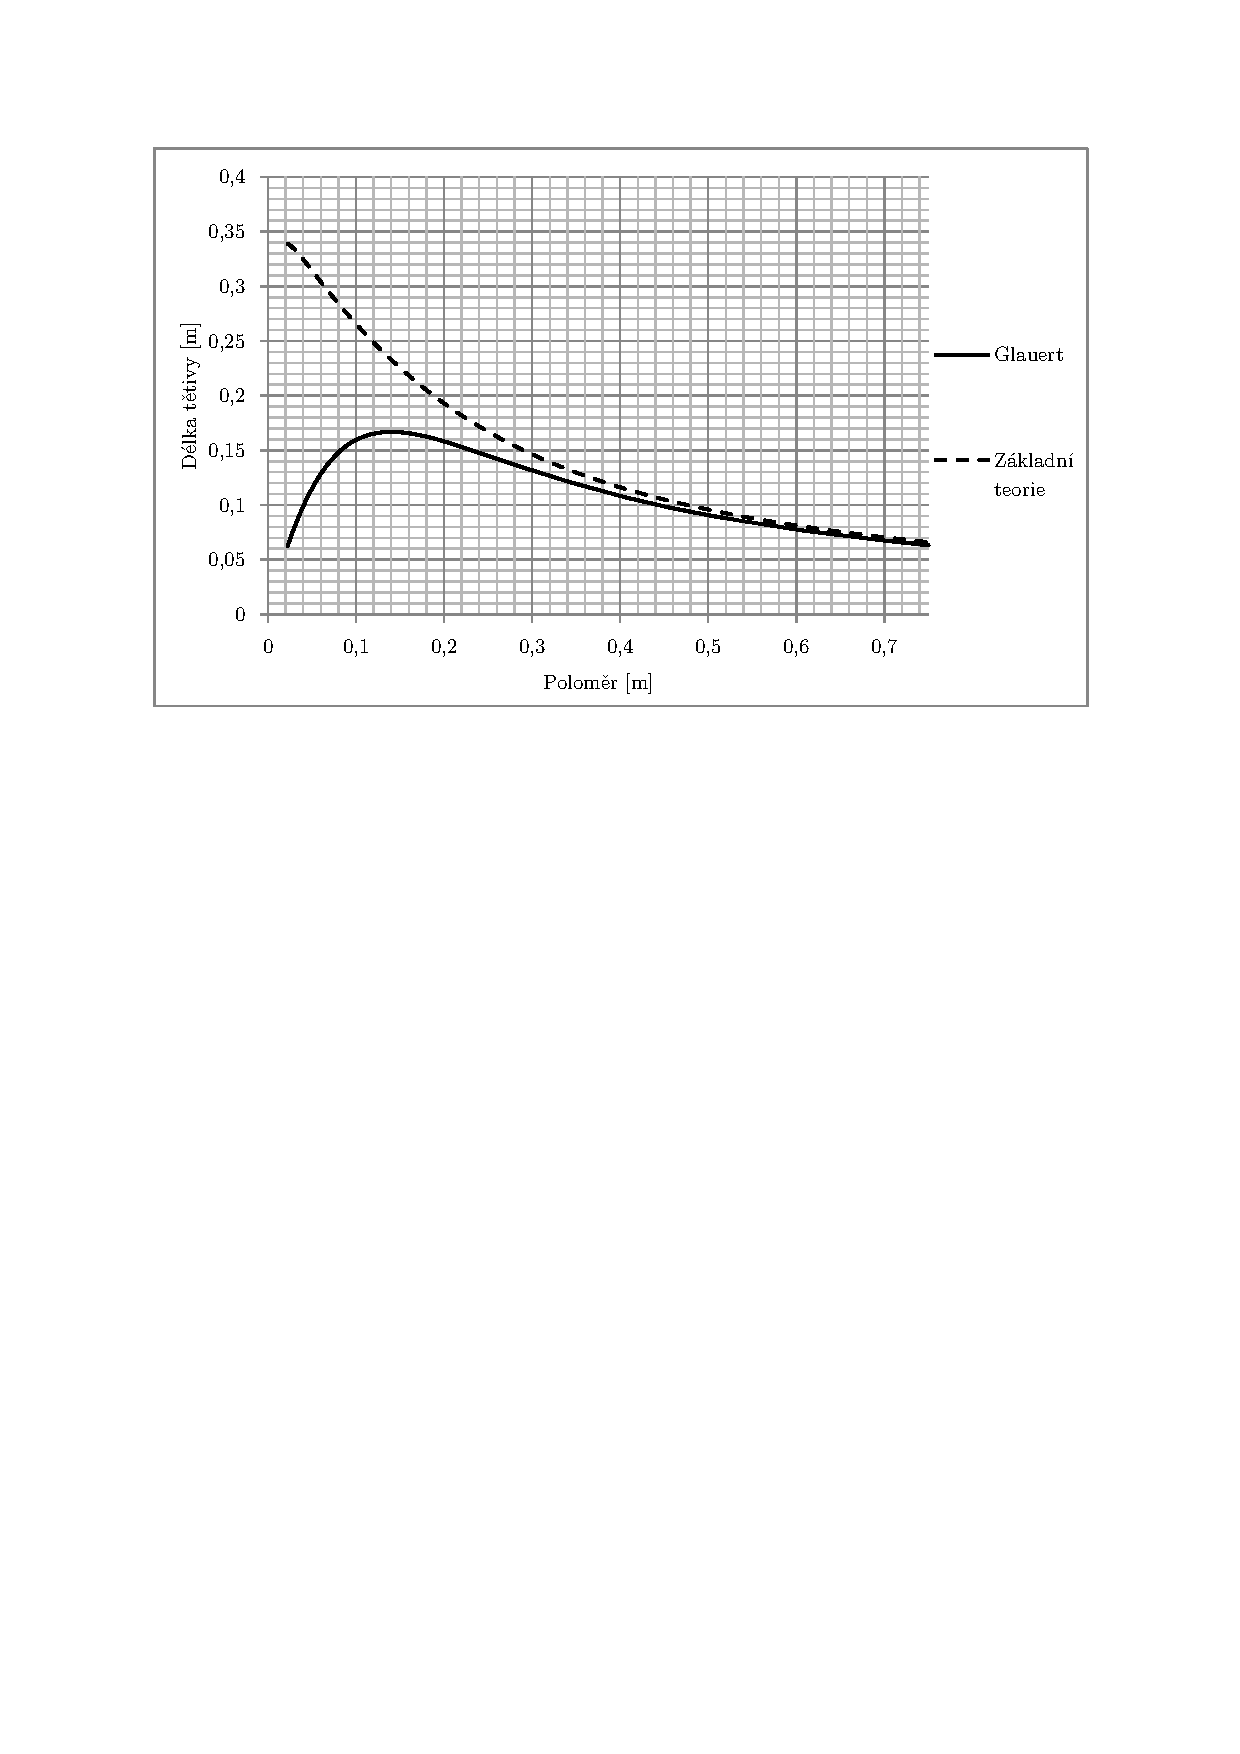
\includegraphics[]{obrazky/grafy/glauert1}
					          %\input{obrazky/rotor2.ipe}
						\caption{Graf porovánává délky tětiv pro zjednodušenou teorii a pro teorii podle Glauerta. List je počítán pro stejné parametry jako v grafu \ref{graf.delka1}}
						\label{graf.glauert1}
					    %\end{center}
		\end{figure}
		\begin{figure}[h]
								%\begin{center}
								\centering
									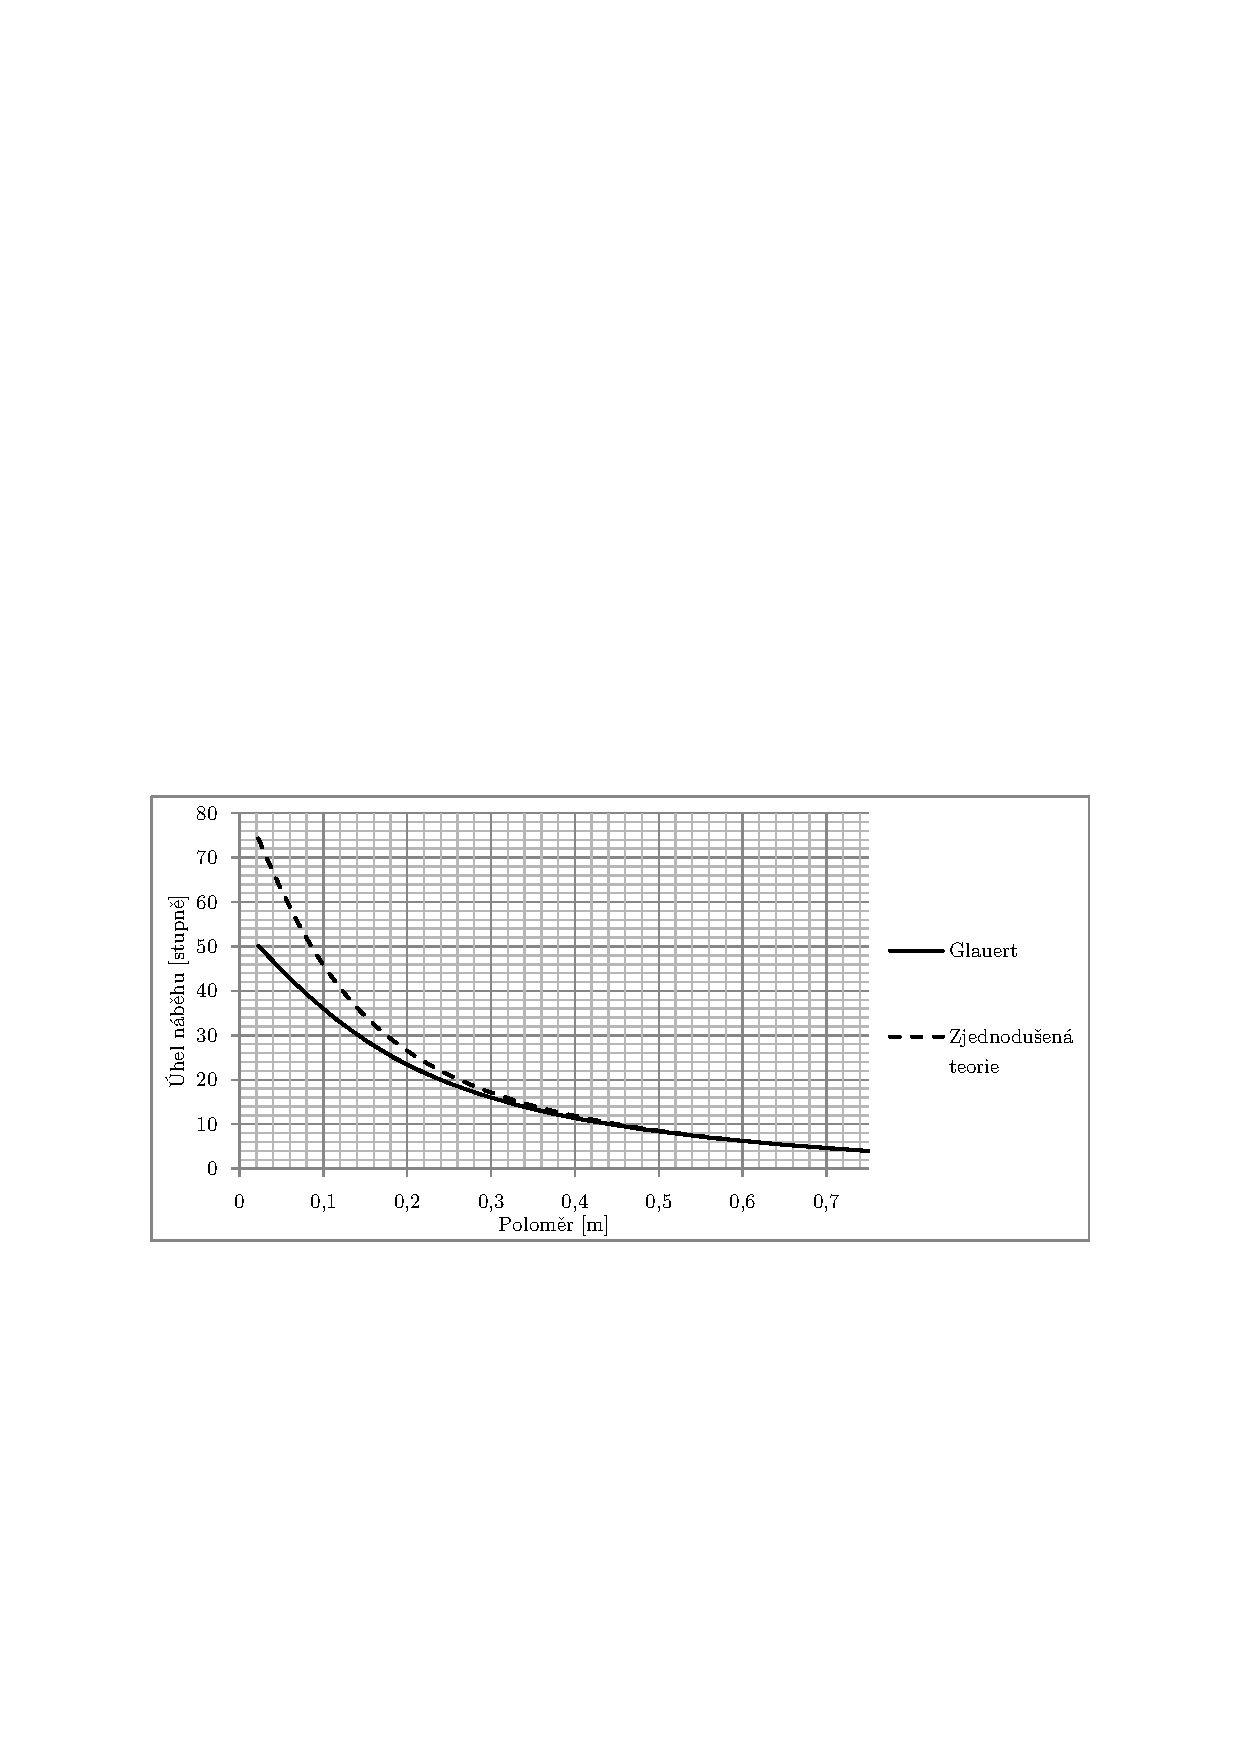
\includegraphics[]{obrazky/grafy/glauert2}
							          %\input{obrazky/rotor2.ipe}
								\caption{Porovnání úhlu náběhu pro zjednodušenou teorii a výpočet podle Glauerta. List je počítán pro stejné parametry jako v grafu \ref{graf.delka1}}
								\label{graf.glauert2}
							    %\end{center}
				\end{figure}
	\chapter{Použití teoretických poznatků}\label{chap:praxe}
Tato kapitola přímo vychází z teorie vysvětlené v kapitole \ref{kap:teorie} a snaží se ji využít při návrhu větrné turbíny.

\section{Parametry návrhu}
V této podkapitole bych rád vytyčil cíle, respektive požadované parametry, navrhované větrné turbíny.

Jak jsem již zmínil v úvodu, čím menší větrná turbína, tím méně je ekonomicky rentabilní. Turbíny s průměrem menším než 5~metrů jsou v podstatě nerentabilní. Proto se v návrhu nebudu omezovat komplikovaností či finanční náročností výroby turbíny. Cílem je navrhnout co nejúčinnější turbínu, která může být umístěna v zástavbě a bude fungovat jako technická zajímavost.

Jelikož bude turbína umístěna v zástavbě, je nutné zvolit rozumnou velikost, aby nebyla příliš rušivá. Čím větší turbína, tím jsou také nižší otáčky při stejné rychloběžnosti. S velkou turbínou se také pojí vyšší zatížení stožáru, který pak musí být kotven např. pomocí lan, což je v zástavbě, resp. na zahrádce, značně omezující. Naopak i malý přírůstek na průměru přidá na výkonu turbíny – výkon turbíny je odvislý od její plochy, přičemž ta roste se čtvercem poloměru. Nakonec jsem se rozhodl pro návrh turbíny s průměrem 2,5~m. Vycházel jsem zde ze zkušeností s~prvním prototypem, jehož průměr 1,5~metru se ukázal jako malý a průměr turbíny přes 3~metry by mohl působit značně rušivě. Navíc již nyní se vyskytly problémy s~manipulací se sestavenou 1,5m turbínou.

Dalším charakteristickým znakem větrné turbíny je počet listů. Zde jsem zvolil 3. Toto číslo bylo zvoleno adekvátně k požadované rychloběžnosti dle tabulky na straně 70 v knize \cite{Rychetnik:Motory}. Navíc vzhled turbíny je „přirozený“ – většině lidí se pod pojmem větrná elektrárna vybaví právě třílistá turbína.

Posledním voleným parametrem turbíny je její rychloběžnost. U prvního prototypu byla zvolena relativně nízká rychloběžnost~4 díky obavám z hluku (při vyšší rychloběžnosti se konce listů pochybují rychle, čímž snadněji vyvolávají hluk). Obavy se ukázaly jako neopodstatněné. Podle grafu na stránkách \cite{ve:ve}\footnote{http://ve.ic.cz/files/teorie/ucinnost.png}  a tabulky 3.1 v knize \cite{Rychetnik:Motory}, leží maximální účinnost třílisté turbíny mezi rychloběžností 5 a 6. Jelikož požadavek na nízkou hlučnost je relativně důležitý, rozhodl jsem se pro jistotu zvolit rychloběžnost 5.

Jelikož není potřeba vytvářet síťové napětí, nebude mít turbína z důvodu jednoduchosti nastavitelné listy pro regulaci otáček. Tím se také zvýší její účinnost.

\section{Výběr profilu}
Prvním krokem při návrhu turbíny hned po stanovení jejích parametrů je výběr turbíny. Z~předchozí teorie vypadá, že stačí vybrat pouze profil s co největším poměrem součinitelů $c_y/c_x$. Výběr profilu však má některá úskalí, která bych v této kapitole chtěl probrat.

\subsection{Reynoldsovo číslo}
V kapitole \ref{kap:zakladprinc} jsem zmínil, že aerodynamické vlastnosti profilu souvisí s podmínkami, ve kterým je provozován. Tyto podmínky charakterizuje Reynoldsdovo číslo \cite{Rychetnik:Motory}, která bylo definováno v rovnici \eqref{rov:13}.

Jedná se pouze o orientační údaj; vlastnosti profilů se na jeho velikosti mění pouze málo. Např. pro profil SG6043 je součinitel $c_y$ pro $Re$ $10^5$ roven 1,415; pro $7,5\cdot 10^4$ 1,408 a pro $5\cdot 10^4$ je 1,389. Tato data byla převzata z \cite{profil}\footnote{http://www.worldofkrauss.com/foils/getpolar/787.dat}. Navíc parametry profilů jsou dostupné pouze pro některá Re.
Abych mohl spočítat $Re$, je nutné odhadnout délku tětivy. Její délka se však výrazně mění. Většinou se však uvažuje délka tětivy u konce listu, která má největší podíl na výkonu. Délka tětivy se v tomto případě pohybuje okolo 10~cm.

Také rychlost obtékání profilu se uvažuje pouze jako obvodová rychlost rotoru, nikoliv jako vektorový součin obvodové rychlosti rotoru a rychlosti větru. Pro vítr o rychlosti 4 $m\cdot s^{-1}$ je~$Re$ \eqref{rov:50}:
\begin{equation}
	\label{rov:50}
	Re=\frac{vl}{\nu}=\frac{v_1\cdot\lambda l}{\nu}=\frac{4\cdot 5 \cdot 0,1}{15\cdot 10^6}\doteq 1,33\cdot 10^5
	\end{equation}
Je tedy nutné vybírat z profilů, které vykazují dobré vlastnosti při $Re$ $1,33\cdot 10^5$.

\subsection{Ideální vlastnosti profilu}
V~tabulkách k~daným profilům, lze zpravidla najít údaj o maximální hodnotě poměru $c_y/c_x$ (též označovaného jako jemnost profilu). Z~čistě teoretického hlediska lze říci, že tento parametr je dostačující.

V praxi však nelze dosáhnout ideálních podmínek. Všechny teorie uvedené v předchozí kapitole předpokládají, že směr relativní rychlosti větru $\beta$ je konstantní. V praxi to však nelze dodržet. Zpravidla nastávají tři nepříznivé situace:
\paragraph{Vítr nevane v celé ploše turbíny stejnou rychlostí.} Tento jev se projevuje hlavně u~velkých turbín. Avšak má vliv i na malé turbíny, zejména v turbulentním prostředí, kde jsou rozdíly rychlostí velké. Zástavba takovým prostředím bezpochyby je.
\paragraph{Turbína je zatížena.} Při přílišném zatížení turbíny se sníží její rychlost otáčení, což vede ke snížení rychloběžnosti a změně směru relativní rychlosti větru.
\paragraph{Turbína se rozbíhá.} Při rozběhu se turbína otáčí pomaleji než je navržena, tudíž její rychloběžnost opět není konstantní a relativní proud vzduchu má opět jiný směr než ideální.\vspace{0.5cm}

Z těchto důvodů je vhodné, aby profil měl co nejpodobnější hodnoty součinitelů $c_x$ a $c_y$ pro co největší rozsah úhlů náběhu – díky tomu bude turbína podávat dobré vlastnosti i při nepříznivých podmínkách. Je také výhodné, aby maximální hodnota jemnosti profilu měla podobné hodnoty od sebe jak v~kladném, tak i záporném směru – důvod je zřejmý. Na grafech \ref{graf.jemnost1}, \ref{graf:jemnost2} a \ref{graf:jemnost3} jsou zobrazeny ilustrační příklady takových průběhů jemnosti profilu.

\begin{figure}[H]
	\centering
	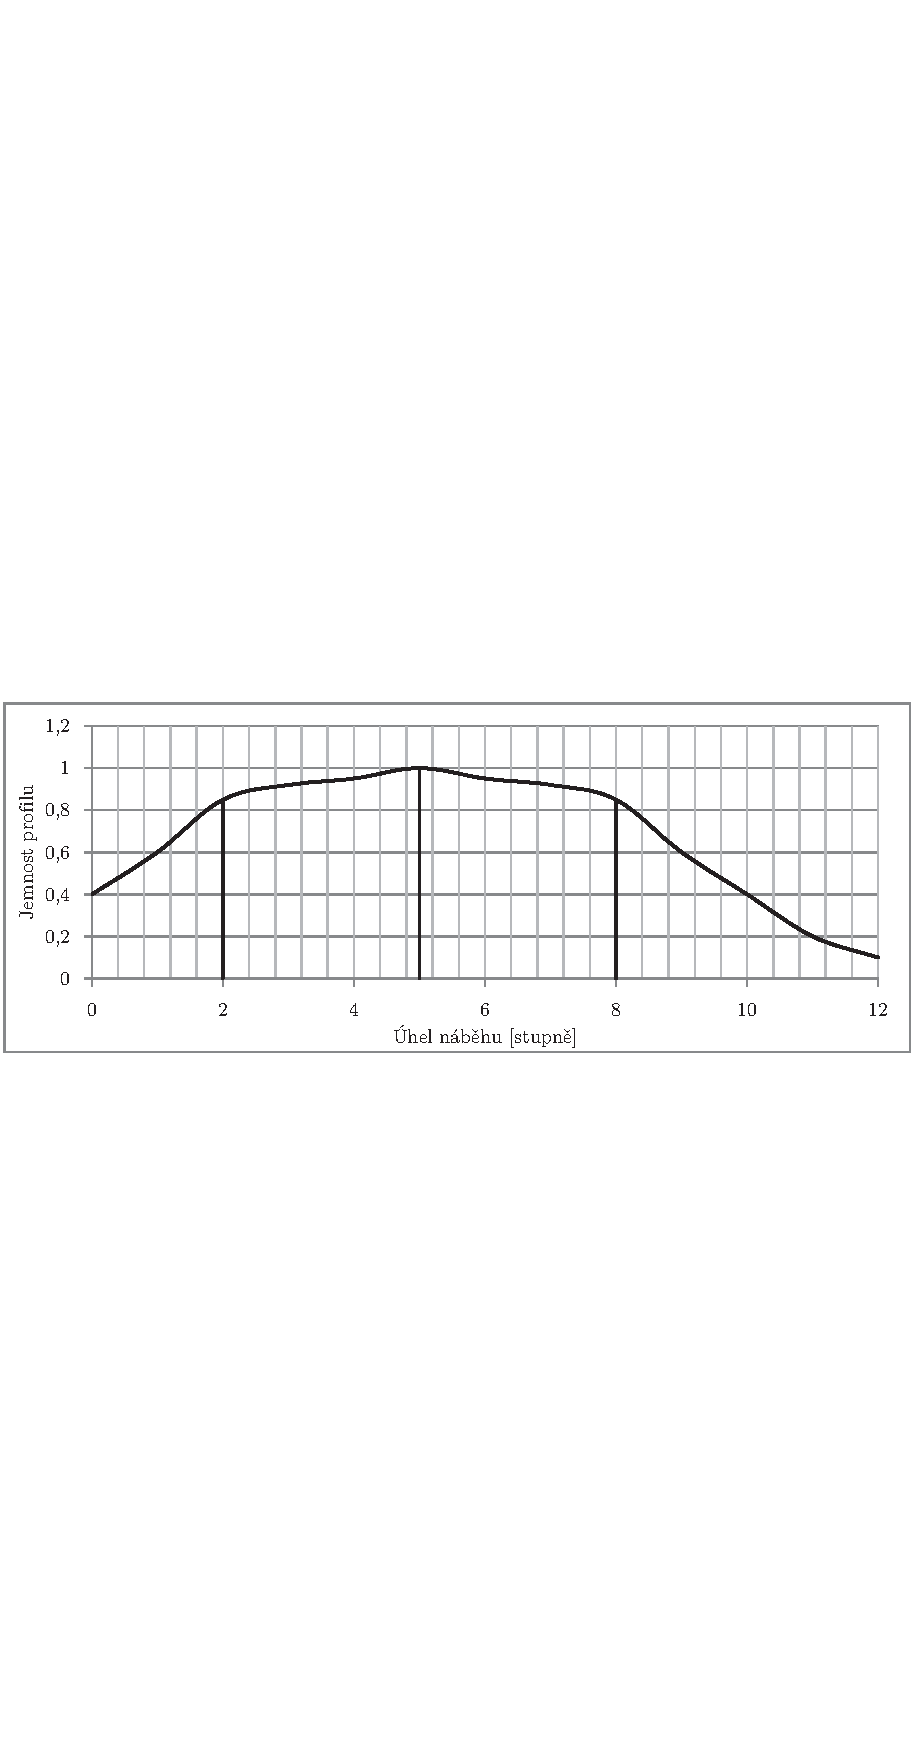
\includegraphics[]{obrazky/grafy/jemnost1p}
	\caption{Graf zobrazuje vhodný průběh jemnosti profilu k úhlu náběhu. Je vidět, že profil dává v~rozmězí $2$–$8\,^{\circ}$ velmi podobné výsledky. Data jsou pouze ilustrační, nejsou založena na žádném existujícím profilu}
	\label{graf.jemnost1}
\end{figure}

	\begin{figure}[H]
	\centering
	\subfigure[Maximálních hodnot jemnosti profil dosahuje pouze na minimálním úseku]{
\includegraphics[]{obrazky/grafy/jemnost2p}\label{graf:jemnost2}}~
	\subfigure[Charakteristika je výrazně asymetrická]{
\includegraphics[]{obrazky/grafy/jemnost3p}\label{graf:jemnost3}}
	\caption{Grafy znázorňují nevhodný průběh jemnosti profilu. Data jsou pouze ilustrační.}
	\end{figure}
	
\subsection{Výběr profilu}
	Ze stránek Airfoil Inverstigation Database \cite{profil} jsem vybral několik na první pohled vhodných profilů. A to profily WORTMANN FX 60-126, EPPLER 395, GOE 481A a SG6043. V této kapitole je na základě výše uvedených kritérií porovnám. Veškerá data o profilech jsou převzata také z těchto stránek.
	\paragraph{WORTMANN FX 60-126}(obrázek \ref{profil:wort}) Tento profil na první pohled zaujme vysokou jemností profilu (graf \ref{profil:wortj}) – 170 při úhlu náběhu $5\,^{\circ}$. Avšak při pohled na průběh jemnosti je jasné, že tento profil není vhodný do nepříznivých podmínek – ideálních hodnot dosahuje pouze na malém intervalu úhlů náběhu, navíc asymetricky.
	\begin{figure}[H]
		\centering
		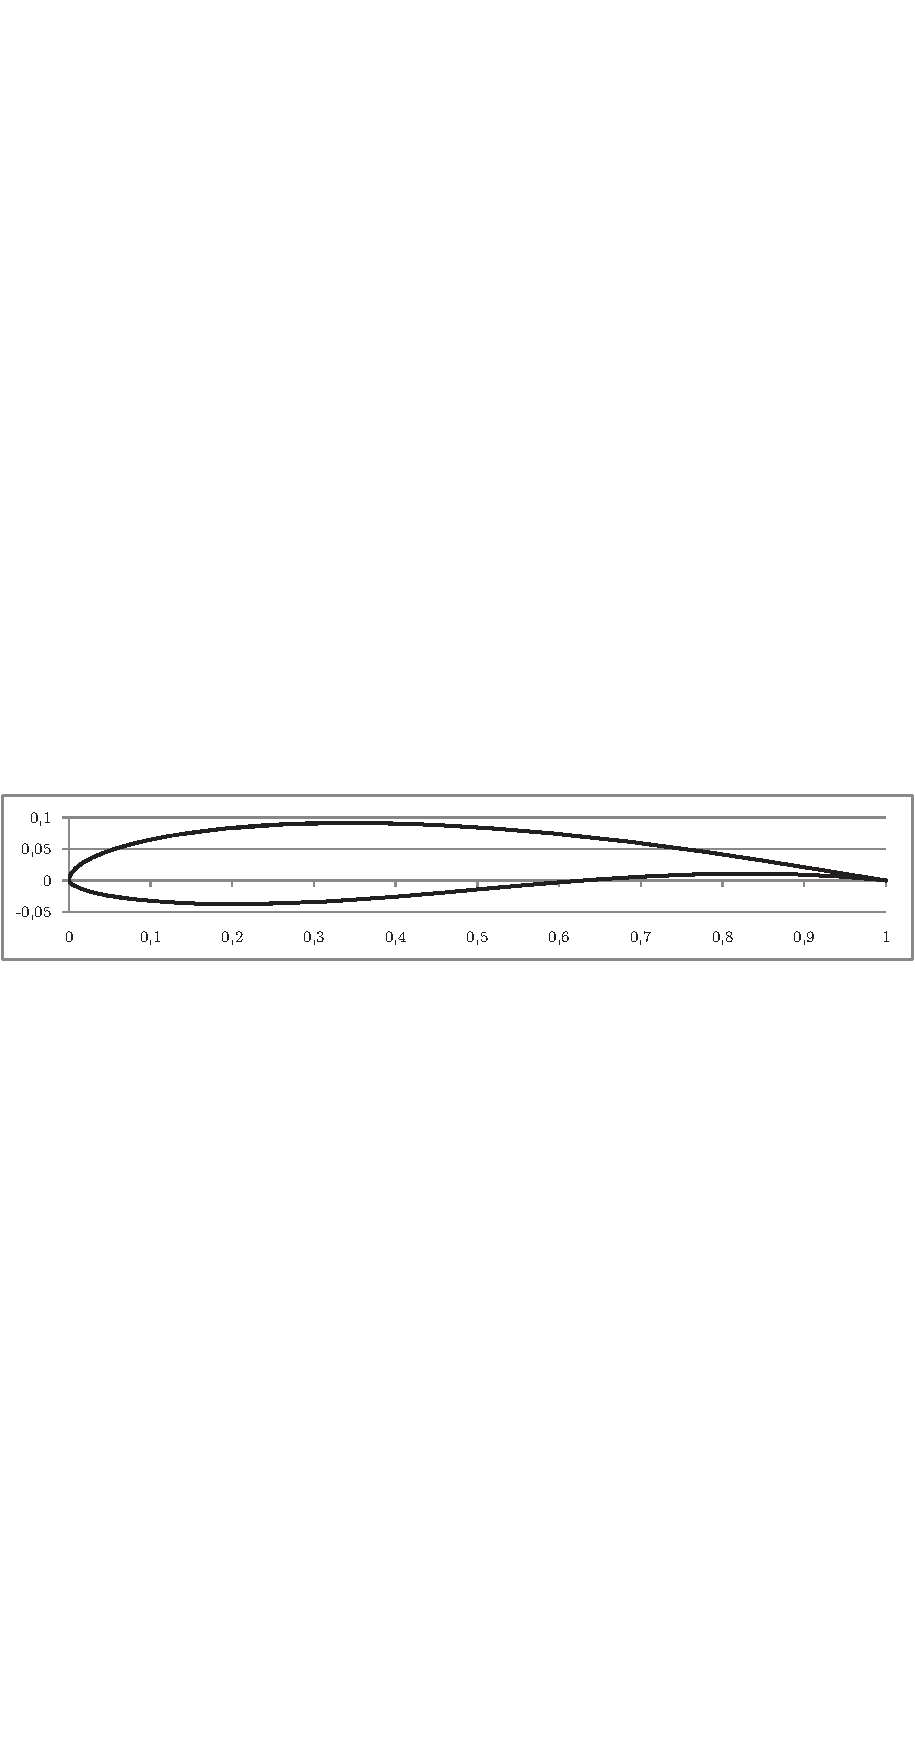
\includegraphics[]{obrazky/grafy/wortmannp}
		\caption{Profil WORTMANN FX 60-126}
		\label{profil:wort}
	\end{figure}
	\begin{figure}[H]
			\centering
			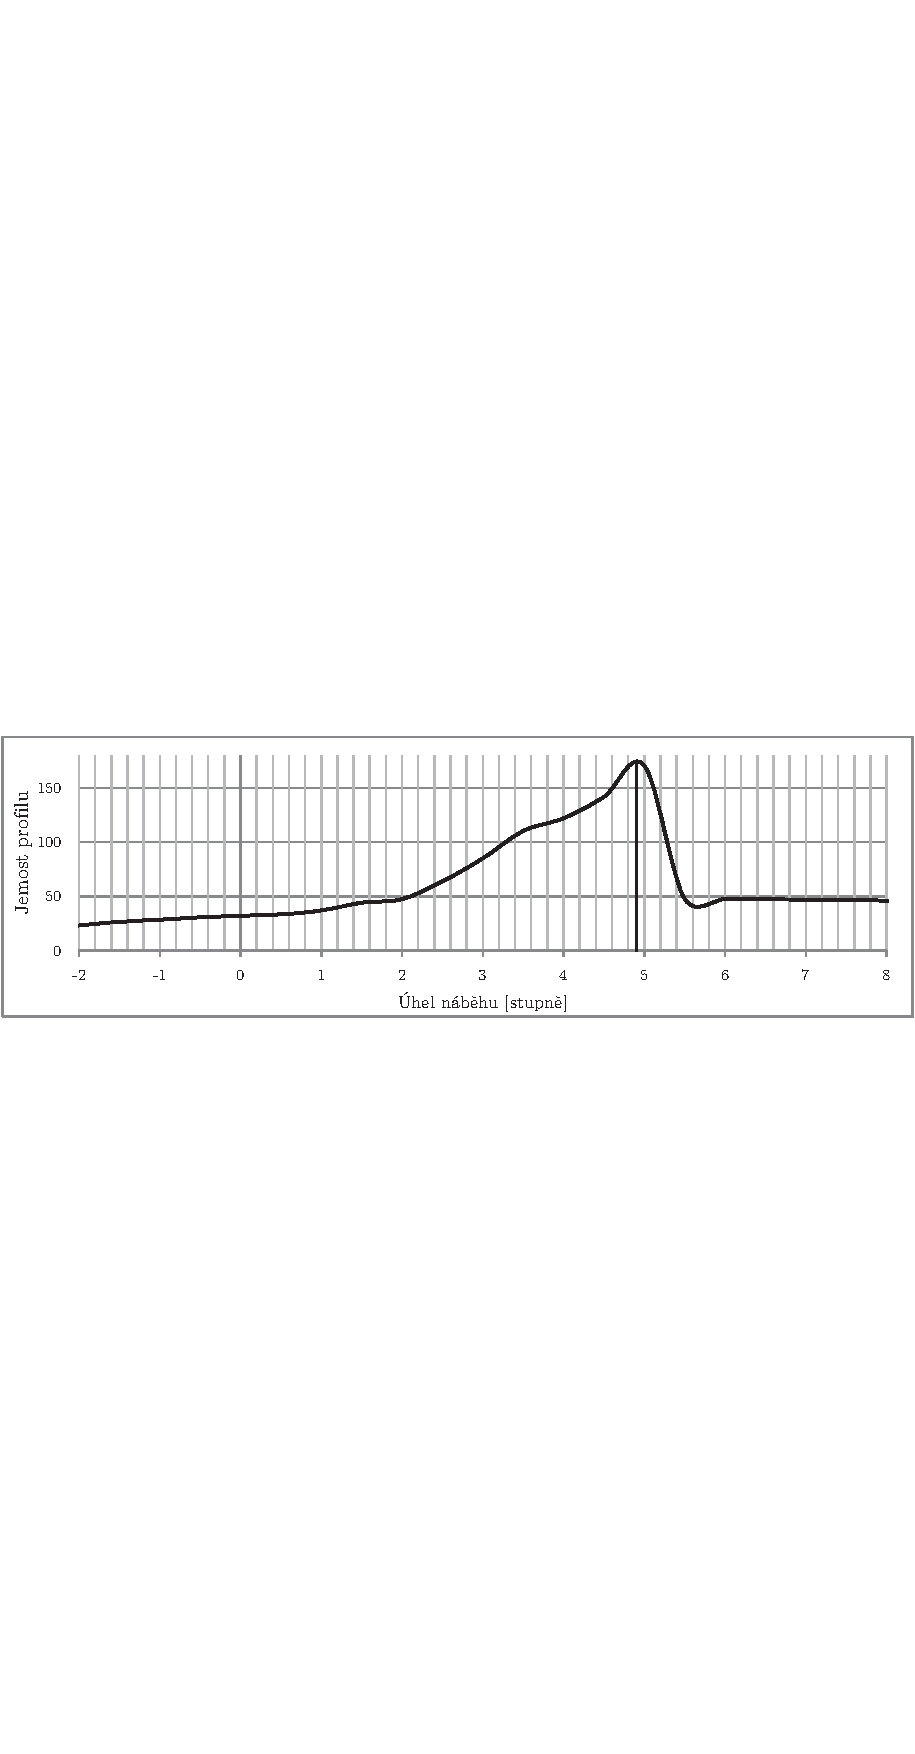
\includegraphics[]{obrazky/grafy/wortmannjp}
			\caption{Jemnost profilu WORTMANN FX 60-126}
			\label{profil:wortj}
	\end{figure}
	\paragraph{EPPLER 395} (obrázek \ref{profil:epp}) Tento profil opět na první pohled lákal vysou jemností (graf \ref{profil:eppj}) – 80. Směrem do záporných hodnot jeho jemnost klesá pozvolna, avšak do kladných prudce klesá. Pro mé podmínky se jedná o nevhodný profil.
	\begin{figure}[H]
			\centering
			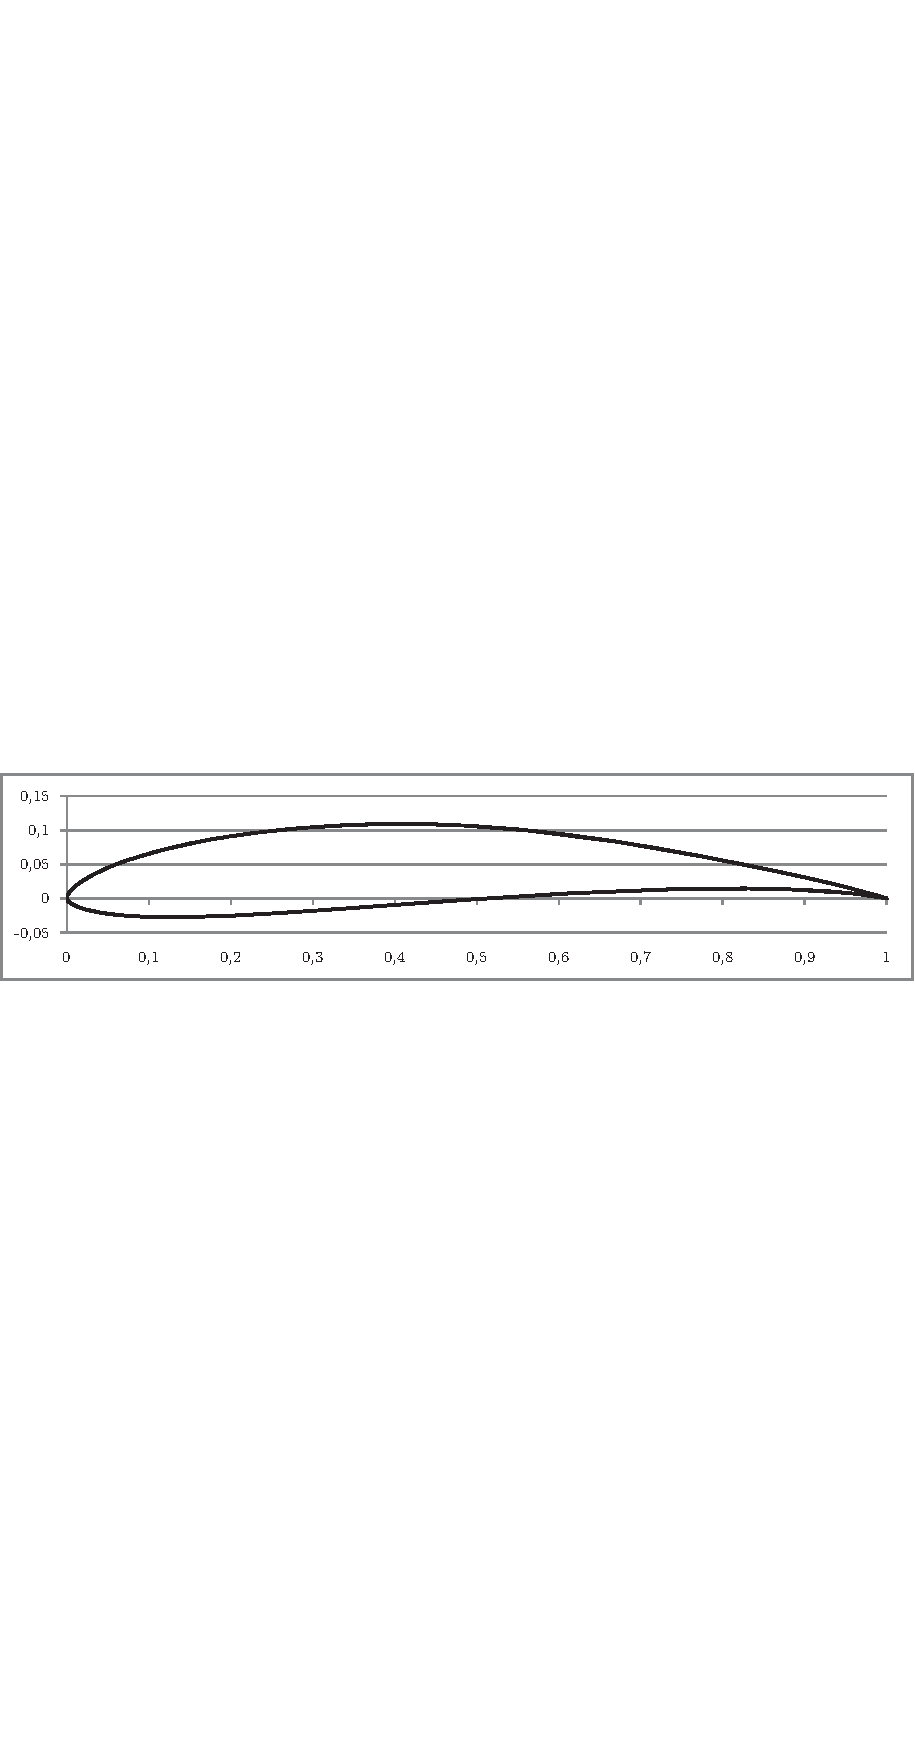
\includegraphics[]{obrazky/grafy/eppp}
			\caption{Profil EPPLER 395}
			\label{profil:epp}
		\end{figure}
		\begin{figure}[H]
				\centering
				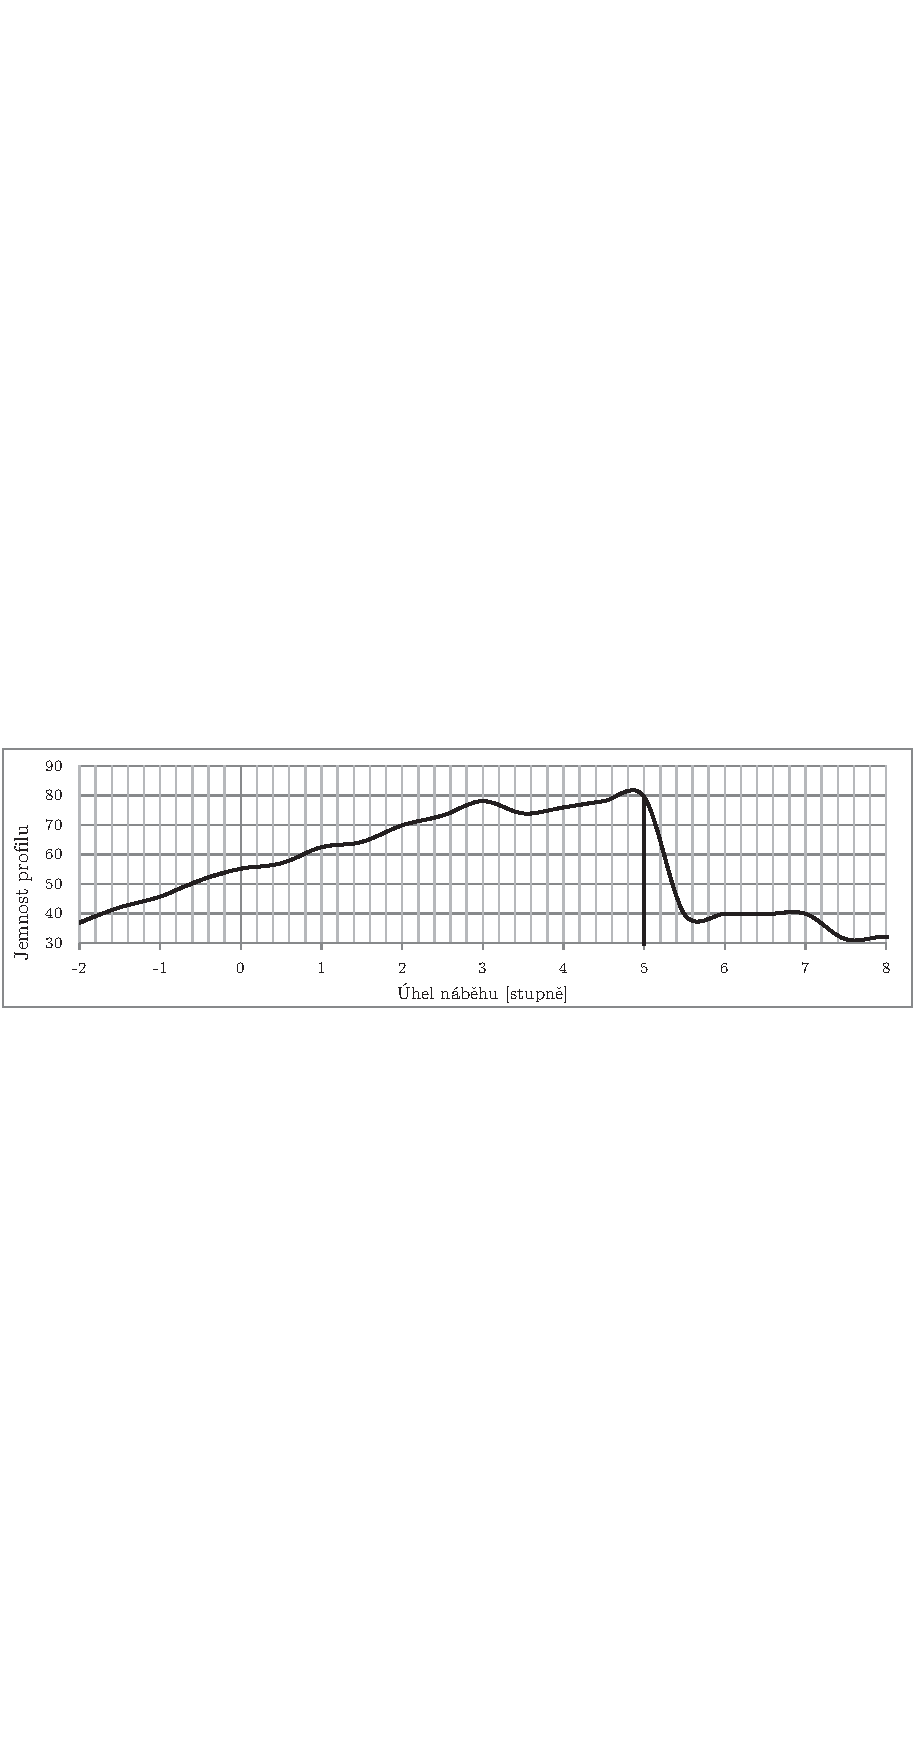
\includegraphics[]{obrazky/grafy/eppjp}
				\caption{Jemnost profilu EPPLER 395}
				\label{profil:eppj}
		\end{figure}
	\paragraph{GOE481A} (obrázek \ref{profil:goe}) Tento profil dosahuje jemnosti 73 a tuto vysokou jemnost udržuje na dlouhém intervalu úhlů náběhu – od 3 do $8\,^{\circ}$ (graf \ref{profil:goej}). Má i relativně velkou tloušťku, což je výhodné pro konstrukci listu.
	\begin{figure}[H]
			\centering
			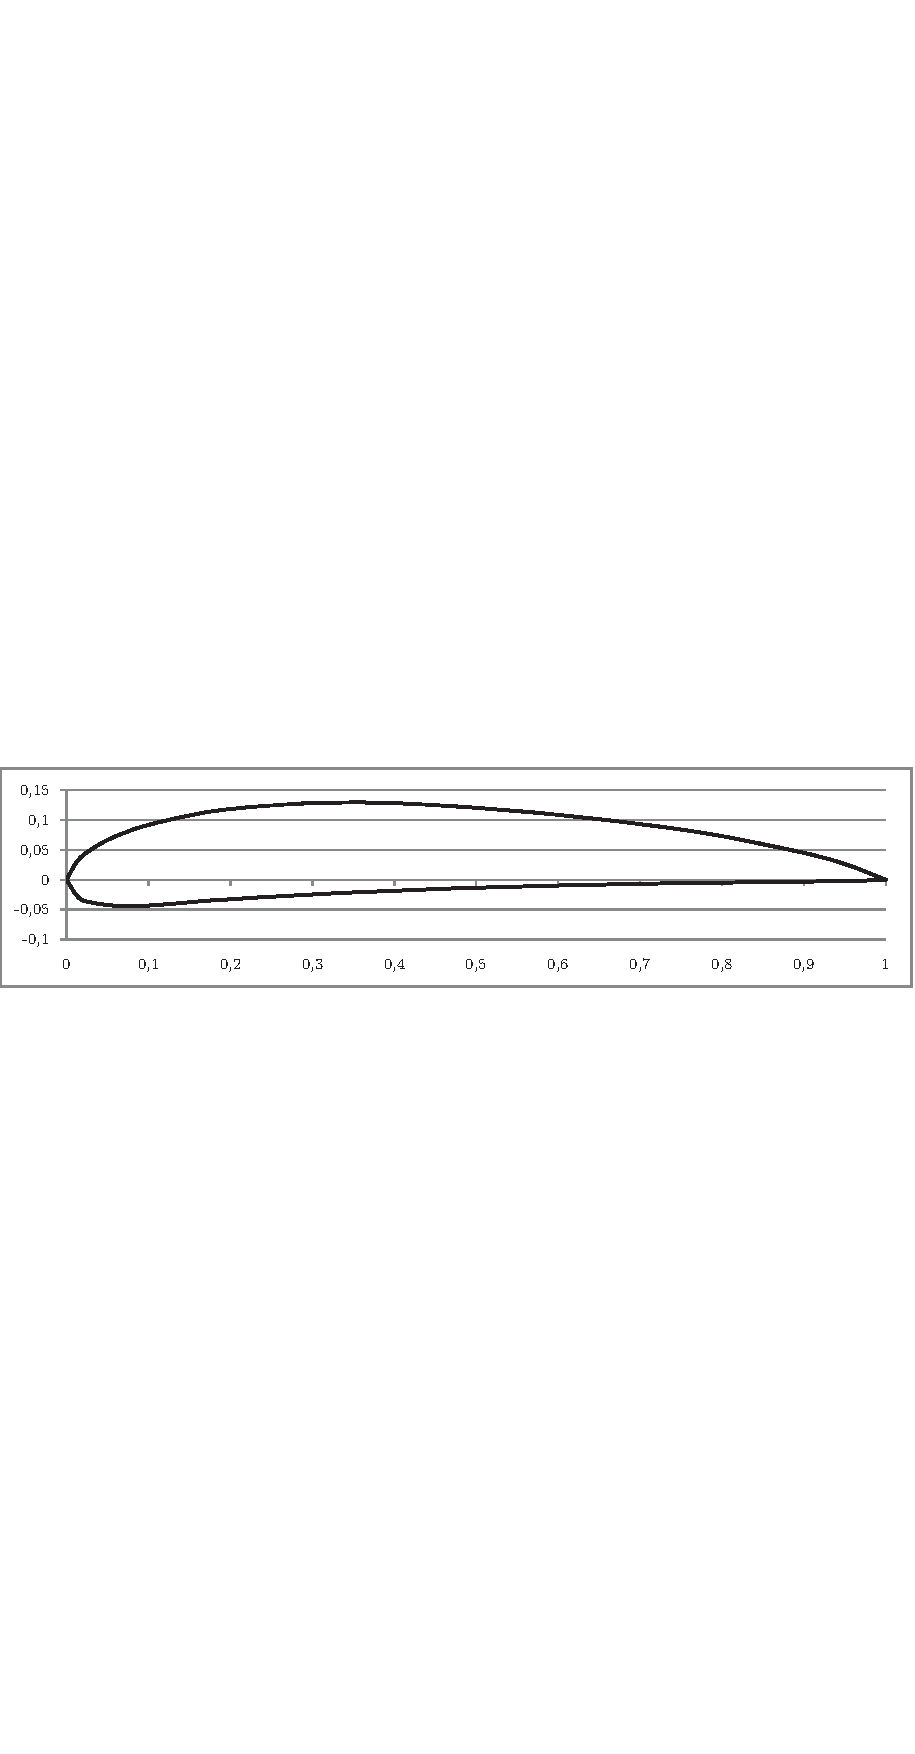
\includegraphics[]{obrazky/grafy/goep}
			\caption{Profil GOE481A}
			\label{profil:goe}
		\end{figure}
		\begin{figure}[H]
				\centering
				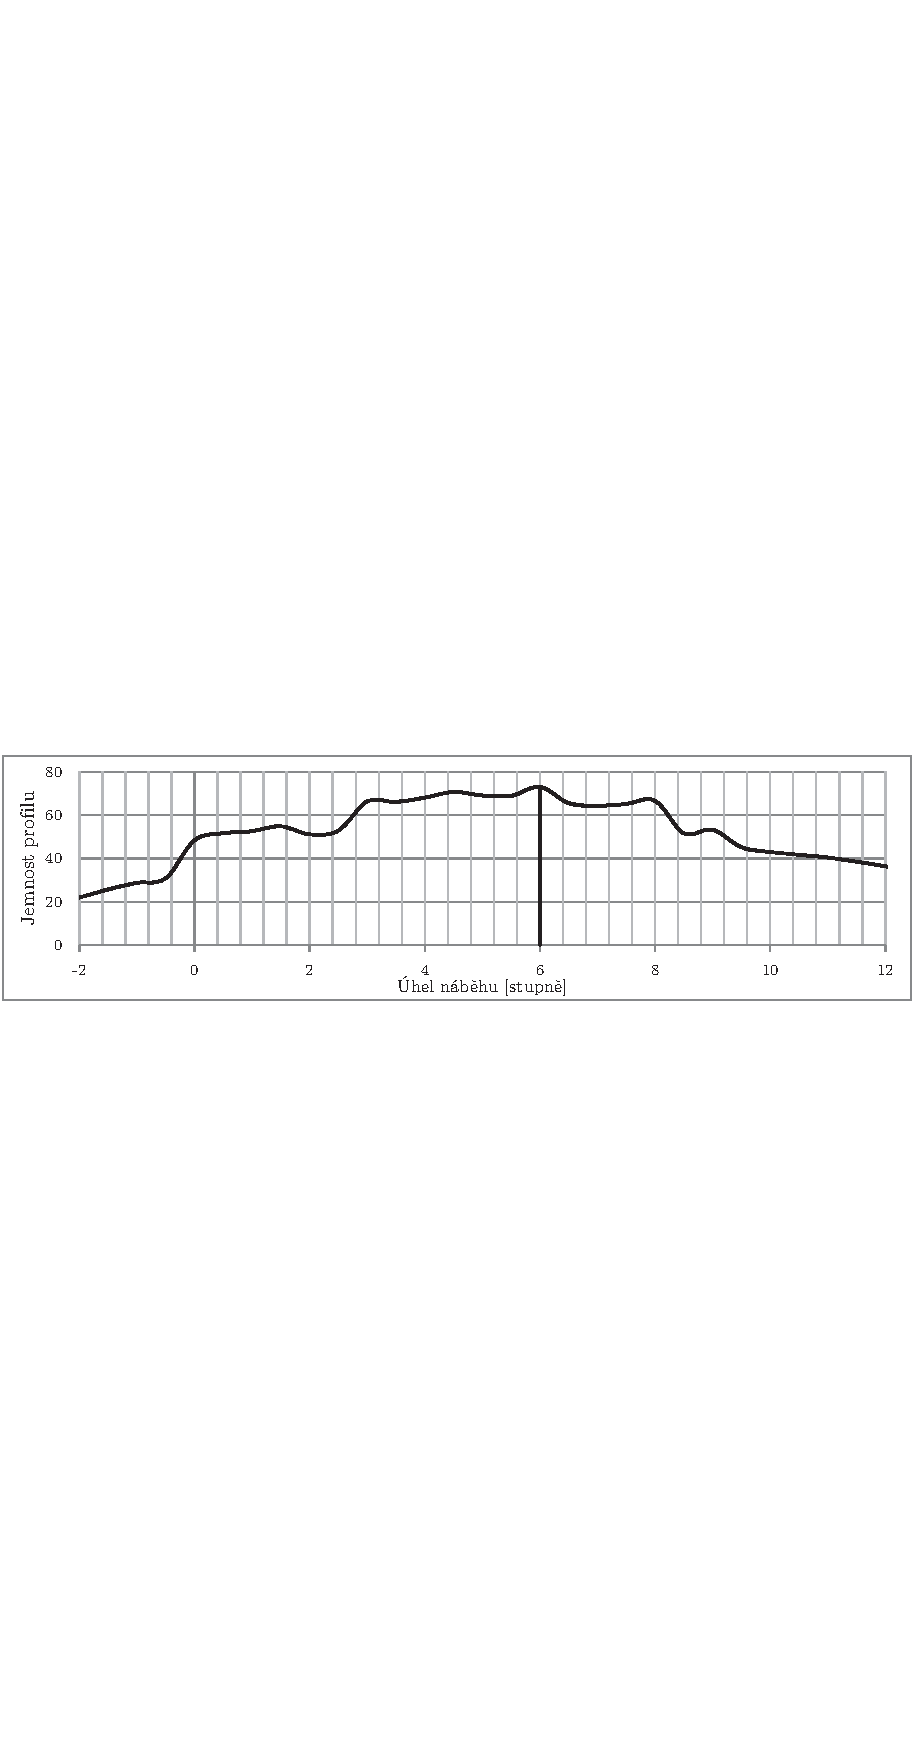
\includegraphics[]{obrazky/grafy/goejp}
				\caption{Jemnost profilu GOE481A}
				\label{profil:goej}
		\end{figure}
		
	\paragraph{SG6043} (obrázek \ref{profil:sg}) Tento profil podobně jako GOE481A dosahuje jemnosti 70 a drží si ji na podobném intervalu (graf \ref{profil:sgj}). Oproti němu však tyto hodnoty nekolísají, což je výhodné. Jeho nevýhodou v porovnání s GOE481A je menší tloušťka.
		\begin{figure}[H]
				\centering
				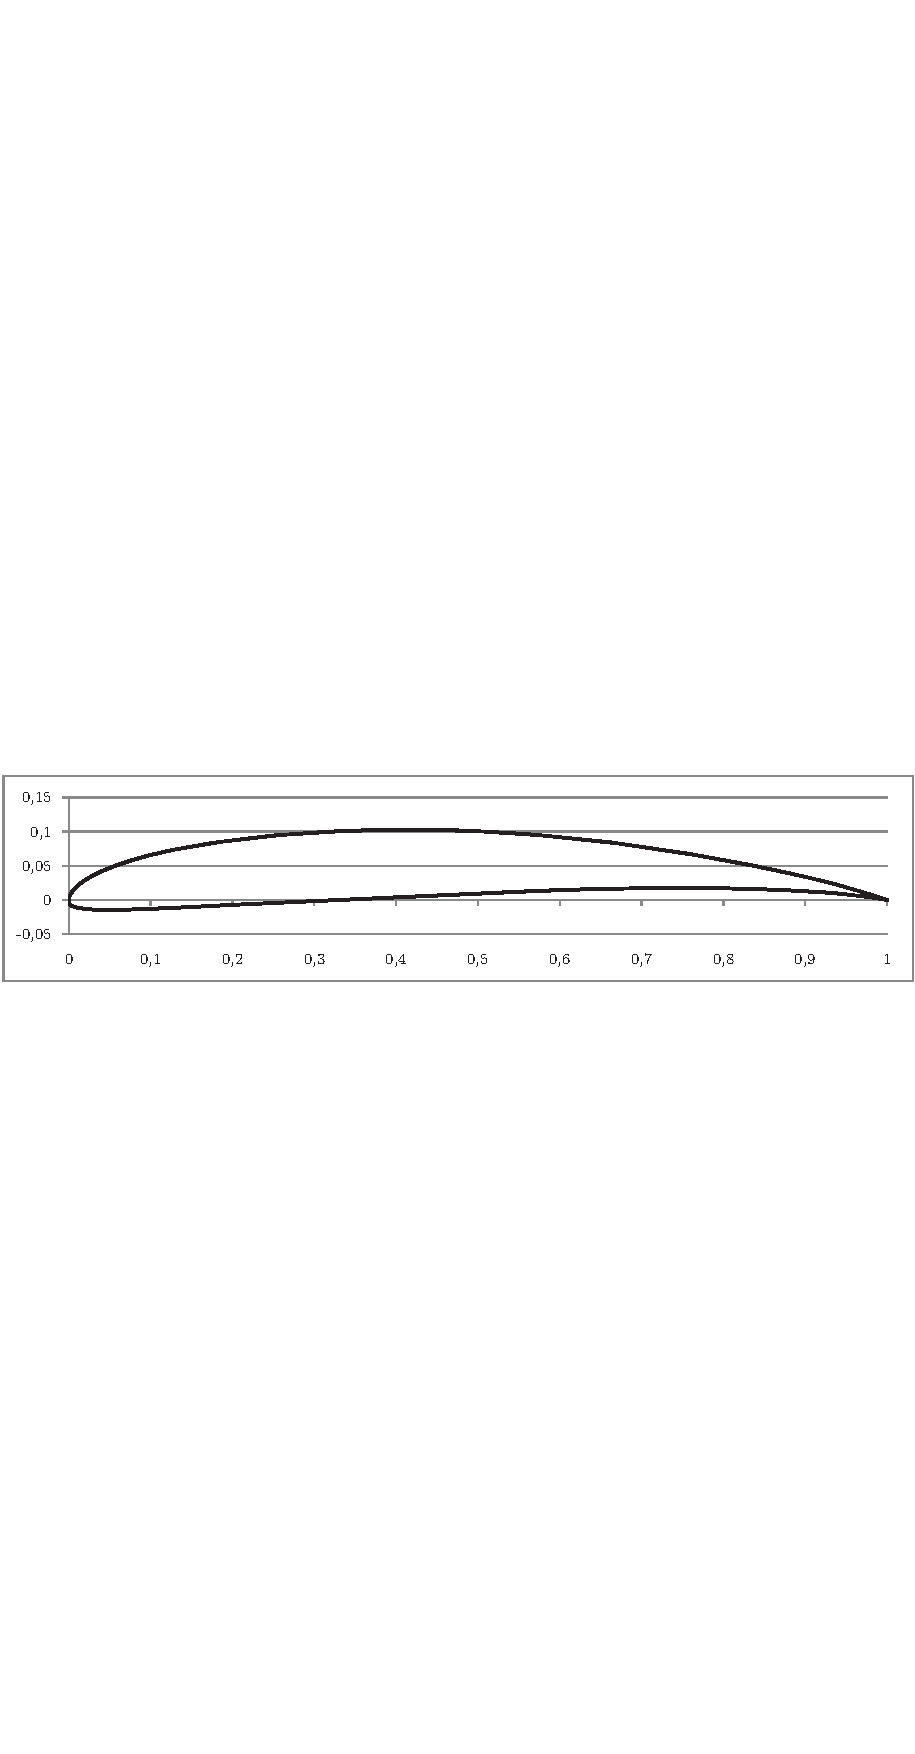
\includegraphics[]{obrazky/grafy/sgp}
				\caption{Profil SG6043}
				\label{profil:sg}
			\end{figure}
			\begin{figure}[H]
					\centering
					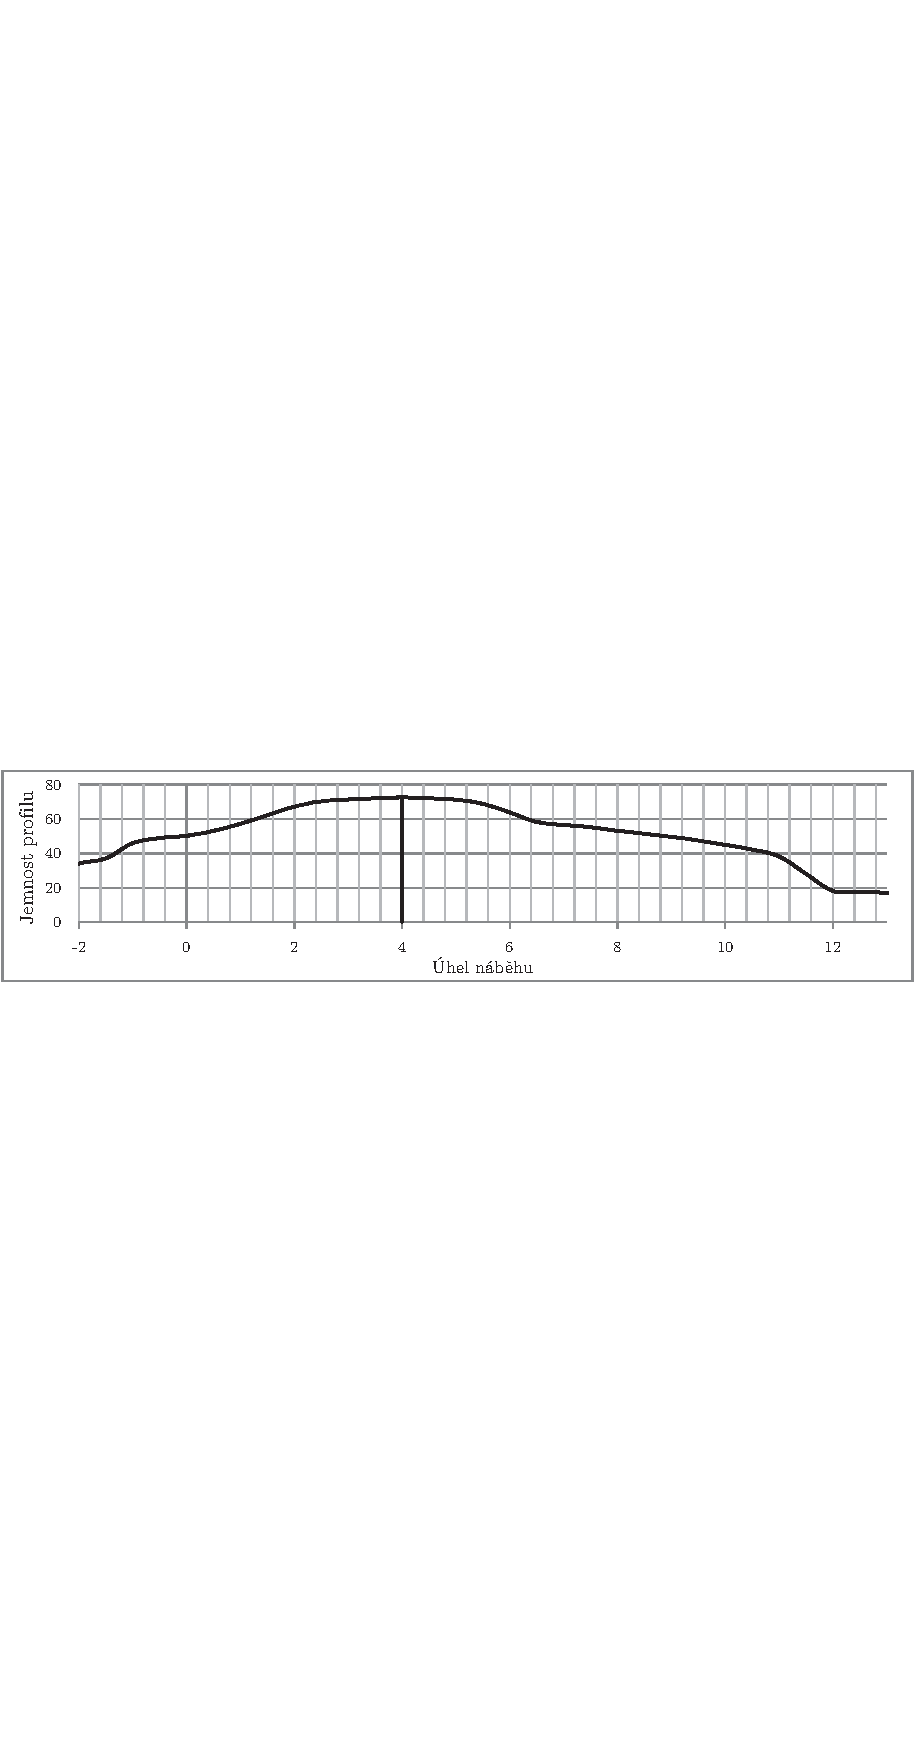
\includegraphics[]{obrazky/grafy/sgjp}
					\caption{Jemnost profilu SG6043}
					\label{profil:sgj}
			\end{figure}
	
	Z těchto profilů se ukázaly jako vhodné pouze 2; a to GOE481A a SG6043. Po zvážení jsem se rozhodl pro SG6043. Jednak má plynulejší průběh jemnosti a navíc s~ním mám už předchozí pozitivní zkušenosti
	
	\section{Postup výpočtu}\label{postup}
	V kapitole \ref{kap:funkce2} jsem zmínil, že výpočet podle Glauerta nelze řešit klasicky. V této kapitole bych rád vysvětlil jednak proč jej nelze řešit klasicky, ale hlavně také jak jej vyřešit.
	
	Při prvním pohledu na problematiku si lze všimnou koeficientů $h$ a $k$, které nejsou nějak definovány. Vystupují jako vstupní hodnota. Tyto koeficienty mohou nebývat nekonečně mnoha platných hodnot. Nás však zajímá hodnota, pro kterou dávají maximální výkon. Je proto vhodné zavést tzv. součinitel výkonu $C_p$ \eqref{rov:51}, který charakterizuje účinnost elementu turbíny na daném poloměru \cite{Rychetnik:Motory}.
	\begin{equation}
		\label{rov:51}
		C_p=\frac{\mathrm{d}P_{turbíny}}{\mathrm{d}P_{vzduchu}}=\frac{\omega\;\mathrm{d}M}{\rho\pi r \; \mathrm{d}rv_1^3}=\frac{\omega^2r^2(1+k)(h-1)}{v_1^2}=\lambda_r^2(1+k)(h-1)
	\end{equation}
	Z této definice by se mohlo zdát, že maximální výkon je nekonečně velký, nesmíme však zapomínat, že součinitelé $k$ a $h$ mají mezi sebou vztah. Tento vztah vychází z~výpočtu úhlu $\beta$ (rovnice \eqref{rov:36}). Pokud tento vztah dosadíme do výsledné rovnice teorie podle Glauerta (rovnice \eqref{rov:49}), získáme vztah \eqref{rov:52}.
		\begin{equation}
			\label{rov:52}
			k= 1 - \lambda_r(h-1)\cot(\beta-\varepsilon)
		\end{equation}
	Z těchto vztahů je patrná cyklická závislost – např. $\beta$ závisí na $k$ a $h$, přičemž $k$ závisí na $\beta$. Koeficient $k$ vychází z~neznámého koeficientu $h$ atd.
	
	Výpočet této soustavy lze provést pouze iteračně. Ručně je takovýto výpočet prakticky neproveditelný, ale na počítači je to otázka zlomků sekund.
	
	Než popíši postup výpočtu, rád bych zmínil ještě jeden poznatek patrný z výše uvedených vztahů. Koeficienty, potažmo i výkonový součinitel, vychází z~rychloběžnosti na poloměru $r$, nikoliv z~rychloběžnosti na konci lopatek. Tudíž budou tyto koeficienty na různých poloměrech různé. Z~tohoto poznatku také plyne to, že nelze sestavit parametrickou rovnici např. pro délku tětivy v~závislosti na poloměru, která by šla zadat přímo do CAD programu. Jednotlivé body této rovnice se totiž opět musí počítat iteračně.
	
	Postup výpočtu jsem zvolil následující. Z rovnice \eqref{rov:51} vyplývá, že $h > 1$, protože proud vzduchu je zpomalován, nikoliv urychlován (tedy $k > 0$) a součinitel výkonu musí být kladný. Pro výpočet je nutné odhadnou výchozí hodnoty. Pro koeficient $k$ jsem vybral výchozí hodnotu $\frac{1}{3}$ podle Betzovy účinnosti. Jelikož jsem se rozhodl iterovat podle $h$, zvolil jsem hodnotu blízkou~1, která je dostatečné malá, aby mohla dále růst a nebyla za maximem součinitele výkonu. Konkrétně $1 + 10^{-5}$.
	
	Z těchto koeficientů vypočítám podle rovnice \eqref{rov:36} úhel $\beta$. Následuje první krok iterace, kdy z~vypočteného úhlu vypočítám podle rovnice \eqref{rov:52} novou hodnotu koeficientu $k$. Z této hodnoty opět vypočítám úhel $\beta$, a tak dále. Tento výpočet opakuji tak dlouho, dokud není rozdíl dvou po sobě jdoucích výsledků menší, než zadaná přesnost.
	
	Až získám přesné hodnoty koeficientu $k$ a úhlu $\beta$ pro danou hodnotu koeficientu $h$, vypočtu součinitel výkonu. Pokud je větší než předchozí, inkrementuji koeficient $h$ o daný inkrement. Pokud je vypočtená hodnota menší, snížím koeficient $h$ o daný inkrement. Pokud má změna součinitele výkonu opačný směr než předcházející, snížím hodnotu inkrementu. Poté znovu začnu určovat hodnotu úhlu $\beta$ a koeficientu $k$, tentokrát však pro novou hodnotu $h$.
	
	Tento postup opakuji do té doby, než inkrement klesne pod zadanou hodnotu (přesnost výpočtu).
	
	Na provedení tohoto výpočtu jsem napsal jednoduchý konzolový program v jazyce C++. Bylo by jej možné napsat i v jiných jazycích, ale C++ je mi nejbližší. Zdrojový kód programu je přiložen v příloze (program je však rozšířen o další funkcionalitu – viz dále). Program byl zamýšlen jako jednoúčelový, na jedno použití. Z toho důvodu program nepřebírá žádný uživatelský vstup a veškerá vstupní data jsou zadávána přímo do zdrojového kódu.
	
	\section{Tvorba CAD modelu}\label{kap:model}
	Předchozí kapitoly shrnují, jak zjistit jednotlivé parametry turbíny, ale neposkytují informace o jejich použití. Tato kapitola popisuje, jak jsem ze získaných dat sestavil základní CAD model turbíny.
	
	CAD model jsem vytvořil v programu SolidWorks, jehož studentskou verzi používám. Model by šel obdobně vytvořit~i~v~ostatních programech.
	
	Základní model jsem vytvořil pomocí funkce \uv{přidat tažením po křivce}, kde jsem táhl aerodynamický profil po přímce za pomoci dvou vodících křivek – jedna běží po náběžné hraně, druhá běží po odtokové hraně.
	
	Z grafů \ref{graf.glauert1} a \ref{graf.glauert2} vyplývá, že křivka není žádnou \uv{běžnou} – nejedná se kružnici, parabolu, či hyperbolu. Pro křivku také dle předchozí kapitoly není možné sestavit parametrickou rovnici, která by se dala přímo zadat do SolidWorks. Jedinou možností je pro tuto křivku určit dostatečné množství bodů a naimportovat ji do SolidWorks. Ten z~těchto bodů následně křivku pomocí splajnu zrekonstruuje.
	
	Pro generování bodů křivky jsem upravil program zmíněný v předchozí kapitole. Program generuje textový sobor, kde jsou tabulátorem oddělené hodnoty zarovnané do sloupců. Tento formát jsem zvolil pro jeho širokou podporu – dá se přímo importovat jak do SolidWorks, tak i~např. do Microsoft Excelu a jiných.
	
	Prvním krokem bylo určení orientace listu v prostoru. Abych respektoval předvolené názvy základních rovin v SolidWorks (přední, pravá a horní), je list umístěn následovně. Z počátku souřadnic, ve směru osy X, vybíhá poloměr. Profil listu je umístěn v rovině YZ, s tím, že osa Y je umístěna proti směru větru.
	
	\begin{figure}[H]
			\centering
			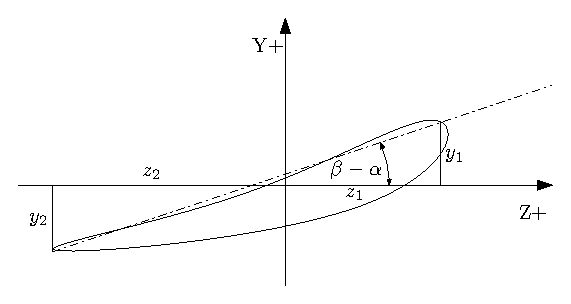
\includegraphics[]{obrazky/profilvprostoru}
			\caption{Umístění profilu v souřadném systému CAD programu.}
			\label{obr.profilosy}
		\end{figure}
	Z obrázku \ref{obr.profilosy} je patrné, jak lze spočítat souřadnice křivky pro náběžnou a odtokovou hranu. Náběžná hrana je křivka s body ve formátu [$r$, $y_1$, $z_1$], odtoková pak [$r$, $y_2$, $z_2$]. Výpočet těchto vzdáleností ukazují vztahy \eqref{rov:53}.
	\begin{eqnarray}
		\label{rov:53}
		y_1=bq\sin(\beta-\alpha) \nonumber \\
		z_1=bq\cos(\beta-\alpha) \nonumber \\
		y_2=b(q-1)\sin(\beta-\alpha)\nonumber \\
		z_2=b(q-1)\cos(\beta-\alpha)
	\end{eqnarray}
	Kde $b$ je délka tětivy, $\beta$ je úhel, který svírá směr relativního proud vzduchu s rovinou rotoru, $\alpha$ je úhel optimálního náběhu daného profilu a $q$ je koeficient vzdálenosti, ve které má profil největší tloušťku. Ten je zde proto, aby se profil v průběhu listu otáčel v místě s největší tloušťkou – cílem je získat co nejvíce prostoru na nosník.
	
	Tato úvaha však má jeden nedostatek – bod, okolo kterého se profil otáčí, neleží uprostřed profilu, ale na jeho tlakové hraně. Je proto nutné ho posunout o polovinu tloušťky profilu ve směru kolmém na tětivu. Tato úprava vypadá následovně\eqref{rov:54}.
	
	\begin{eqnarray}
		\label{rov:54}
		y_1=bq\sin(\beta-\alpha)+\frac{1}{2}bt\cos(\beta-\alpha) \nonumber \\
		z_1=bq\cos(\beta-\alpha)-\frac{1}{2}bt\sin(\beta-\alpha) \nonumber \\
		y_2=b(q-1)\sin(\beta-\alpha)+\frac{1}{2}bt\cos(\beta-\alpha)\nonumber \\
		y_2=b(q-1)\cos(\beta-\alpha)-\frac{1}{2}bt\sin(\beta-\alpha)
	\end{eqnarray}
	Kde $t$ je tloušťka profilu v~procentech délky tětivy profilu.
	Pro profil SG6043 je koeficient $q$~roven 0,33 a koeficient $t$~0,1 (patrno z tvaru tohoto profilu).  Použitím takto vypočtených křivek náběžné a odtokové hrany v prvku \uv{přidat tažením po křivce} vznikne následující model listu, potažmo celého rotoru (obrázky \ref{obr.model1} až \ref{obr.model3}).
	
	\begin{figure}[H]
				\centering
				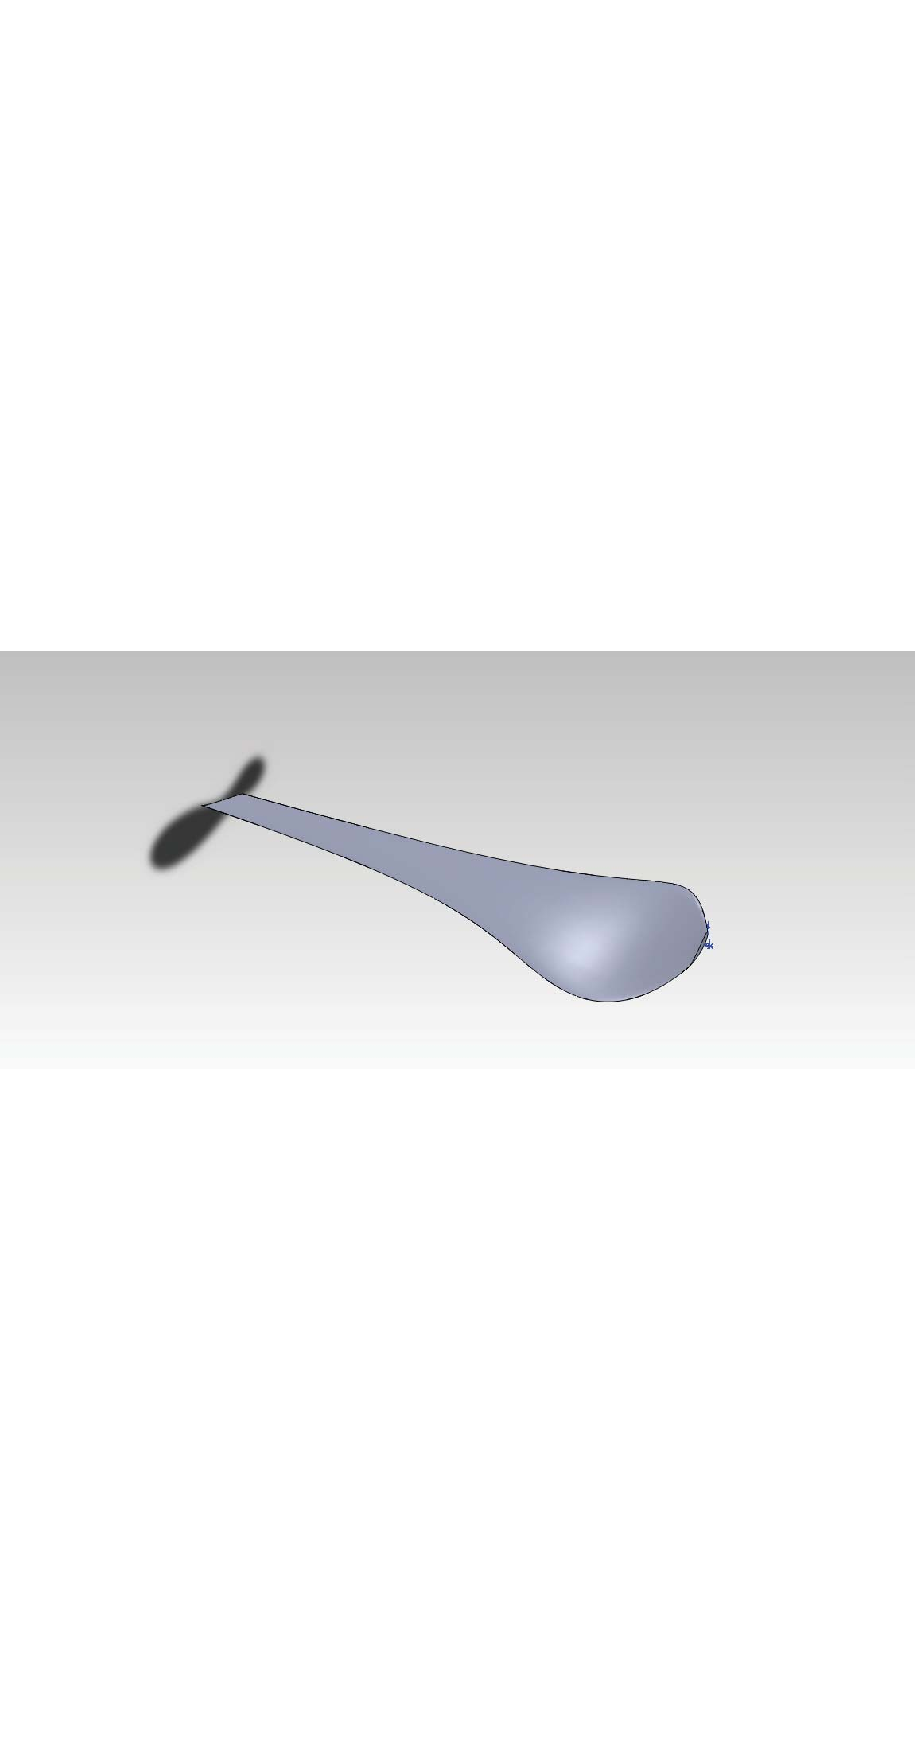
\includegraphics[]{obrazky/rotor/listp}
				\caption{Celkový pohled na rotorový list.}
				\label{obr.model1}
	\end{figure}
	
	\begin{figure}[H]
					\centering
					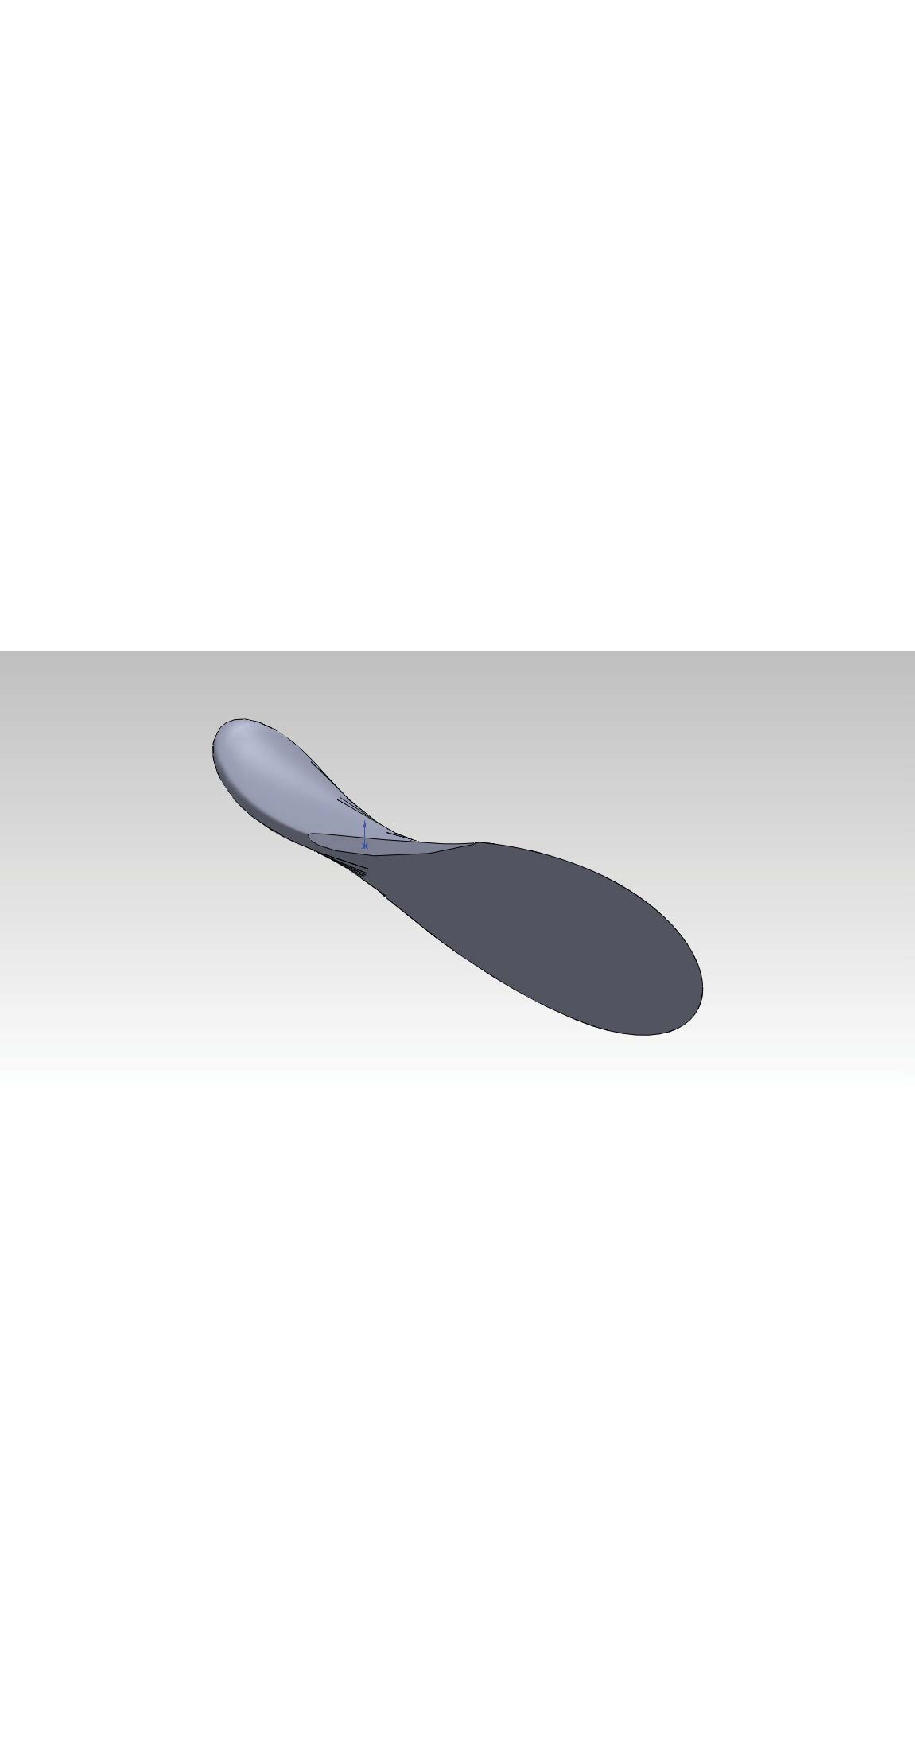
\includegraphics[]{obrazky/rotor/list2p}
					\caption{Pohled na list kolmo na pravou rovinu. Je zde patrný různý úhel náběhu a délka tětivy.}
					\label{obr.model2}
		\end{figure}
	\begin{figure}[H]
					\centering
					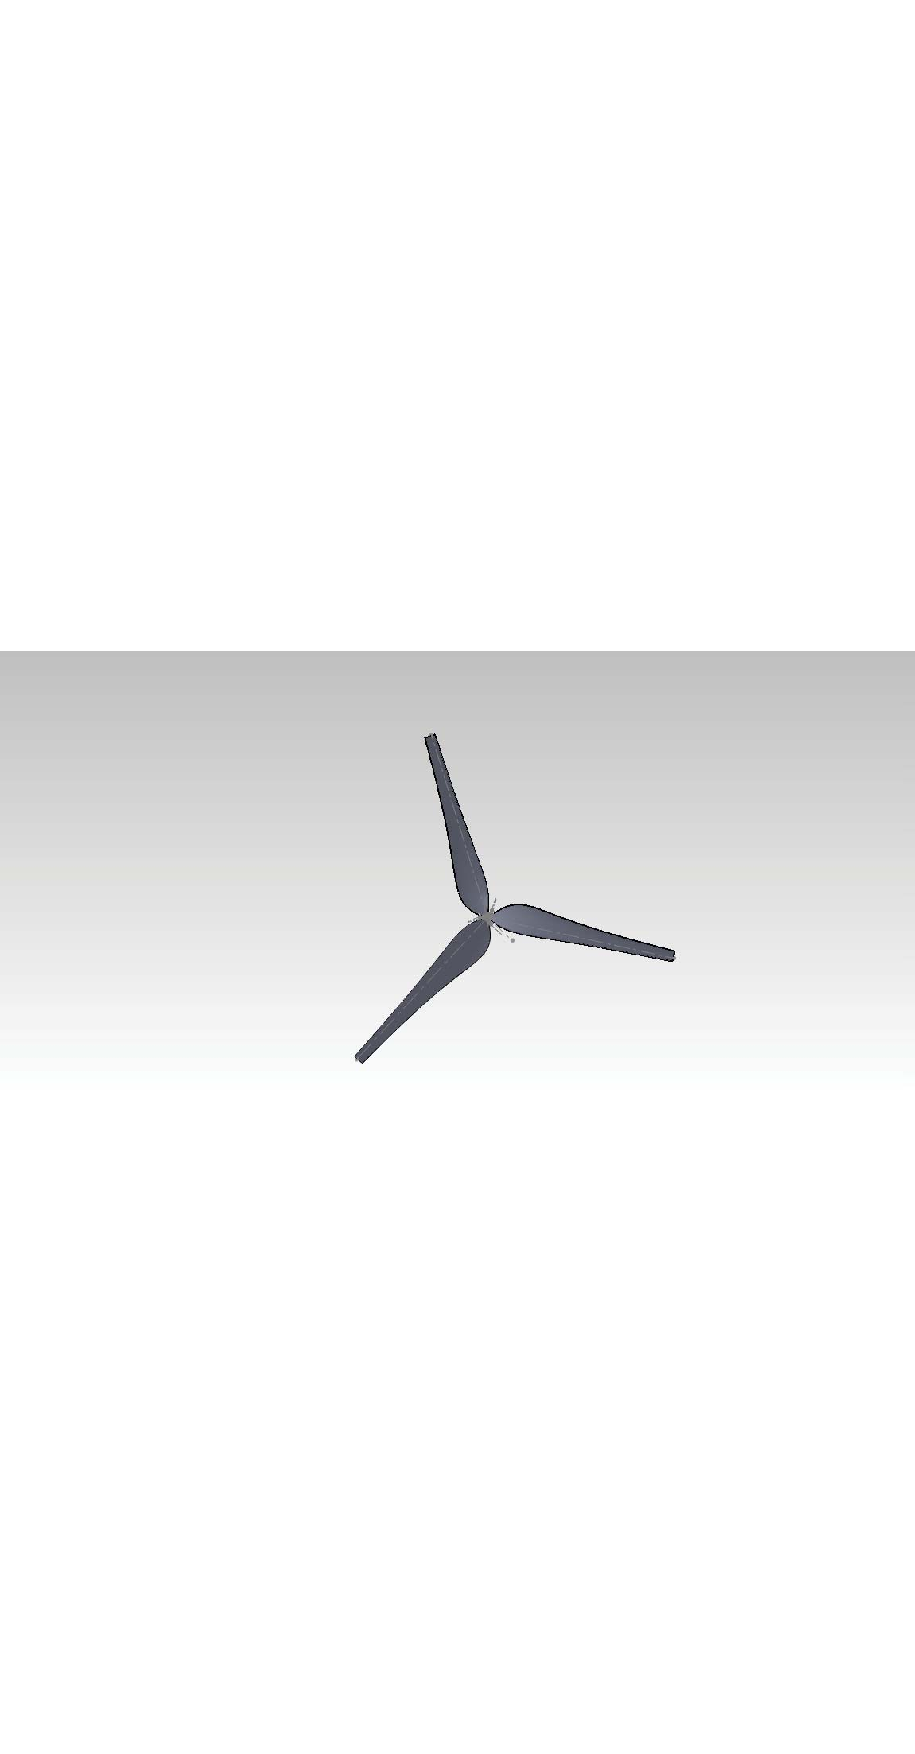
\includegraphics[]{obrazky/rotor/celekp}
					\caption{Pohled na celou turbínu složenou pouze ze 3 listů.}
					\label{obr.model3}
		\end{figure}
		
	\section{Parametry turbíny}
	Výše vytvořený model je teprve začátek návrhu. Potřebuje ještě několik úprav. Před jejich provedením bych však ještě rád uvedl parametry takto navržené turbíny.
	
	Data shrnuji v následujících třech tabulkách. Jsou vypočtena pro rychlosti větru 5~$m\cdot s^{-1}$ (tabulka \ref{tab:r5}), 10~$m\cdot s^{-1}$ (tabulka \ref{tab:r10}) a 25~$m\cdot s^{-1}$ (tabulka \ref{tab:r25}), což dle Beaufortovy stupnice odpovídá mírnému větru, čerstvému větru a vichřici.
	
	Data byla vypočtena pomocí tabulky v Microsoft Excelu pro jednotlivé elementy listu o~tloušťce 6,25~mm. Následně byly tyto hodnoty sečteny. Veškeré vztahy pro výpočet daných hodnot jsou uvedeny v kapitole \ref{kap:funkce2}. Hodnoty v~tabulkách jsou zaokrouhleny na celá čísla.
	\begin{table}[H]
		\centering
		\begin{tabular}{|l|l|}
		\hline
		Rychlost větru	&	5~$m\cdot s^{-1}$\\ \hline \hline
		Výkon vzduchu procházejícího turbínou	&441 $W$\\ \hline
		Axiální síla	&	69 $N$\\\hline
		Moment síly ohýbající list	&	32 $N\cdot m$\\\hline
		Síla roztáčející turbínu	&	15 $N$\\\hline
		Krouticí moment	&	11 $N\cdot m$\\\hline
		Otáčky rotoru	&	160 $min^{-1}$\\\hline
		Užitný výkon turbíny	&	176 $W$\\\hline	
		\end{tabular}
		\caption{Tabulka parametrů trurbíny pro rychlost 5~$m\cdot s^{-1}$}\label{tab:r5}
	\end{table}
	
		
		\begin{table}[H]
				\centering
				\begin{tabular}{|l|l|}
				\hline
				Rychlost větru	&	25~$m\cdot s^{-1}$\\ \hline \hline
				Výkon vzduchu procházejícího turbínou	&55 223 $W$\\ \hline
				Axiální síla	&1 734 $N$\\\hline
				Moment síly ohýbající list	&	481 $N\cdot m$\\\hline
				Síla roztáčející turbínu	&	390 $N$\\\hline
				Krouticí moment	&	262 $N\cdot m$\\\hline
				Otáčky rotoru	&	796 $min^{-1}$\\\hline
				Užitný výkon turbíny	&21 796 $W$\\\hline	
				\end{tabular}
				\caption{Tabulka parametrů trurbíny pro rychlost 25~$m\cdot s^{-1}$}\label{tab:r25}
			\end{table}
	
	Z těchto dat údajů si lze udělat představu jednak o podávaném výkonu a účinnosti, ale také hlavně o technických požadavcích na celou konstrukci. Je důležité si povšimnout, jak velká je síla působící na uložení, tedy i na stožár, a jak prudce roste. Stejně tak roste síla, která působí na list a ohýbá ho, potažmo ho vylamuje~z uložení v náboji. Všechny tyto parametry rostou s~třetí mocninou rychlosti větru. Důležité je uvažovat i působení odstředivé síly na listy, která roste \uv{pouze} s~druhou mocninou rychlosti větru. Tu však nelze spočítat, jelikož není známa konstrukce, a tudíž i hmotnost listu.
	
	Z těchto tabulek také vyplývá fakt, že turbína nutně potřebuje regulační zařízení, které ji při silném větru odstaví z~provozu. Reálný a bezpečný provoz je možný pouze pro rychlosti větru do 10–13~$m\cdot s^{-1}$.
	
	\chapter{Další kroky v návrhu}\label{chap:kroky}
V předchozí kapitole jsem vytvořil základní model rotorového listu. Tento list však má spoustu nevyjasněných prvků, které Gluertova teorie nepokrývá. V této kapitole bych se na ně chtěl zaměřit a probrat je.

\section{Oblast kolem středu, startovatelnost}
Ve většině konstrukcí amatérských větrných turbín si lze všimnout, že autoři záměrně vypouští část listu blízko osy otáčení. Např. v knize \cite{Crome:Technika} autoři vypouští polovinu poloměru. Obdobně i různí autoři uvedení v knize \cite{Hallenga:Elektrarna} vypouští oblast kolem středu.

Tato oblast je vypouštěna nejen díky nízkému výkonu (viz. graf \ref{graf.vykon}), ale také díky dlouhé tětivě, tudíž i větší spotřebě materiálu. Navíc profil v tomto místě omezuje nosnou konstrukci.
\begin{figure}[H]
	\centering
	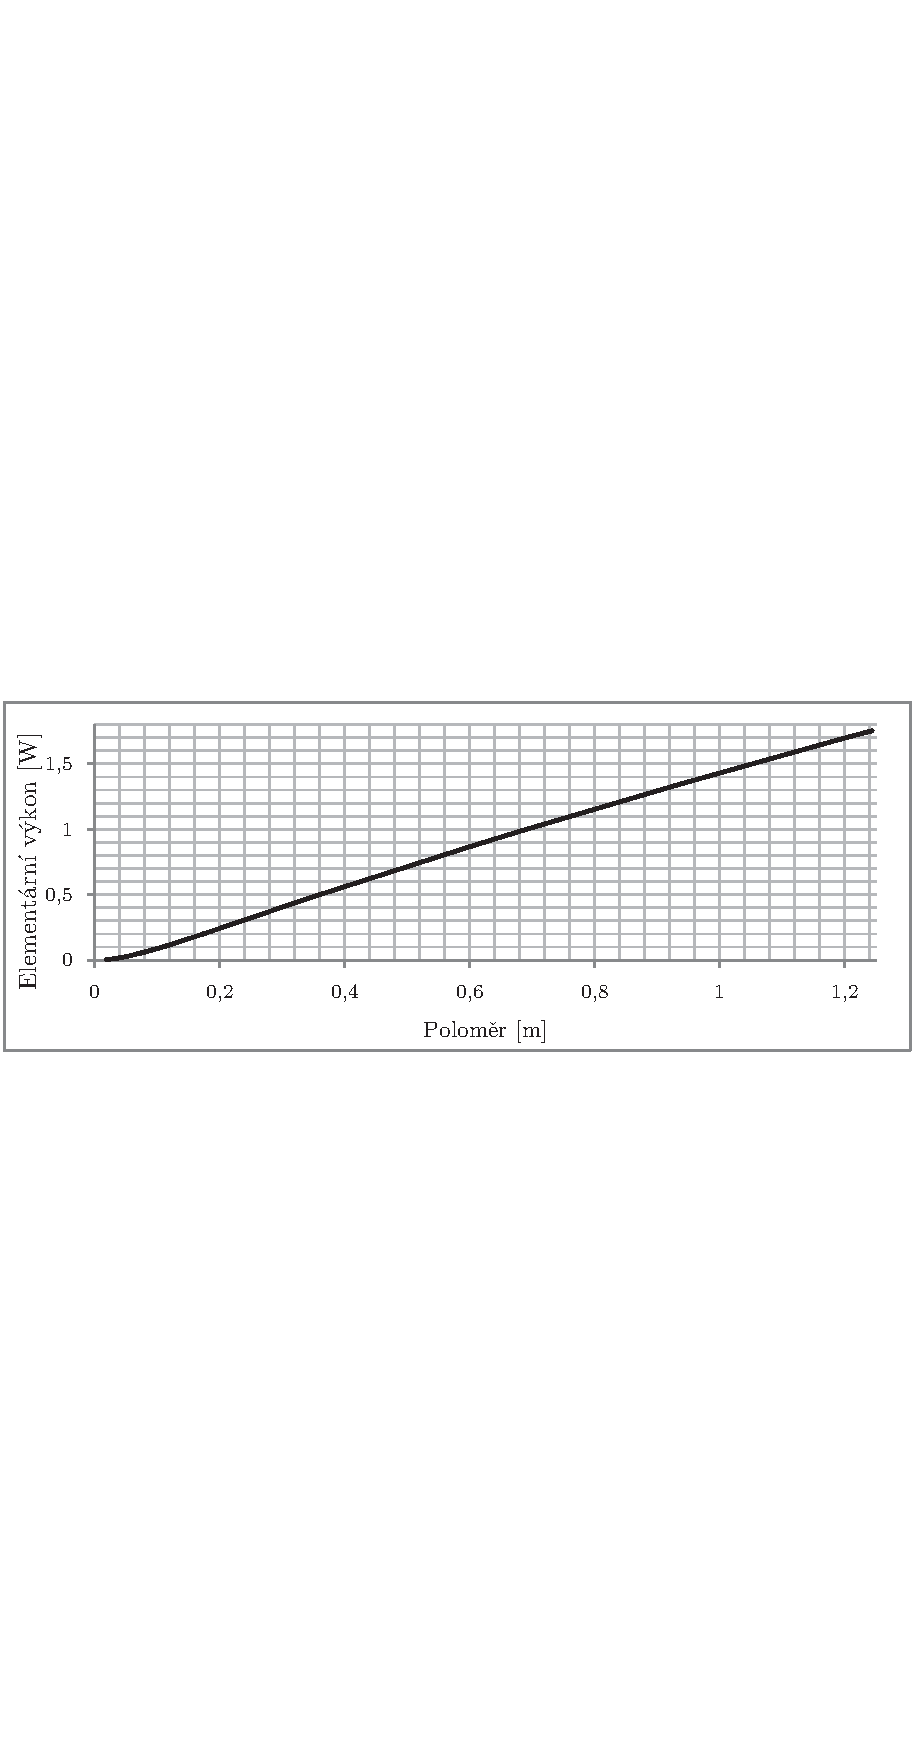
\includegraphics[]{obrazky/grafy/vykonp}
	\caption{Výkon jednotlivých elementů na poloměru $r$}
	\label{graf.vykon}
\end{figure}
V mém návrhu tuto oblast nevypouštím, jelikož se nejvíce podílí na startovatelnosti, která je v turbulentním prostředí důležitá. Na první pohled tato informace vypadá jako nesmysl – síla zde působí na krátké páce a vyvolává malý krouticí moment. Podstata startovatelnosti spočívá jinde.

Veškeré teorie uvažují konstantní rychloběžnost, která však při rozběhu rotoru nenastává. Rotor má menší (resp. nulové) otáčky díky čemuž se mění i směr relativní rychlosti proudu vzduchu a profil není ofukován pod optimálním úhlem, tudíž na něm nevzniká tak velký vztlak (naopak narůstá odpor). Tato odchylka se se vzrůstající rychloběžností zvětšuje. A právě v~oblasti blízko osy rotace je rychloběžnost jednotlivých elementů listu velmi malá, díky čemuž je i~odchylka od ideálního úhlu náběhu malá. K lepší startovatelnosti také významně pomáhá profil, který má charakteristiku podobnou grafu \ref{graf.jemnost1}. Profil je \uv{tolerantnější} k úhlu náběhu a podává dobré výsledky i při nekonstantní rychloběžnosti.

Jelikož má tato oblast listu relativně malou obvodovou rychlost $u$, nezpůsobí zde změna tvaru profilu příliš velký rozdíl v~jeho vlastnostech. Proto je výhodné v této oblasti zvýšit tloušťku profilu a získat více prostoru pro nosnou konstrukci. Tuto změnu tloušťky jsem však do mého CAD modelu zatím nezanesl – ještě nejsou přesně známy technické detaily ohledně realizace rotorových listů.

\section{Zakončení listů}
Gleurtova teorie, stejně jako i ostatní, přepokládají, že rotor má nekonečný počet nekonečně tenkých lopatek. V praxi se však ničemu takovému nelze přiblížit.

Malý počet lopatek se projevuje aerodynamickými ztrátami. Příčinu těchto ztrát lze vysvětlit rozdílným tlakem na tlakové a podtlakové straně aerodynamického profilu. Díky tomuto rozdílu se vzduch na konci listu \uv{přelévá} z tlakové strany na podtlakovou ve snaze tento rozdíl vyrovnat. Tím uděluje proudu vzduchu rotační složku a na konci lopatky tak vzniká tzv. indukovaný vír. Tento vír snižuje vztlakovou sílu na konci listu a je také jednou z příčin hlučnosti větrných turbín.

Nenašel jsem žádnou literaturu, která by se problémem indukovaných vírů u větrných turbín zabývala. Literaturu zabývající se snížením ztrát u křídel letadel lze najít, avšak není příliš podrobná. Většinou jsou v ní indukované víry pouze zmíněny a možnosti, jak je omezit, jsou uvedeny pouhým výčtem. Nenašel jsem nikde popis, jak má např. vypadat winglet, aby měl správnou funkci.

Rozhodl jsem se proto jít experimentální cestou. Jelikož jsou však praktické pokusy časově, materiálně a technicky náročné, rozhodl jsem se využít CFD simulace.

Nesnažil jsem se o odvození teorie, pouze jsem chtěl zjistit, jak lze list rotoru ukončit, aby se snížily indukované ztráty (a potenciálně i hlučnost). Připravil jsem si šest různých zakončení rotorového listu, která jsem následně otestoval v simulaci. Inspiraci pro tato zakončení jsem čerpal z různých zdrojů. Od křídel dopravních letadel, přes fotografie větrných elektráren až po RC modely.

Jako simulační software jsem použil studentskou verzi Autodesk Simulation Multiphysics. Původně jsem plánoval použít open-source projekt OpenFOAM\footnote{http://www.openfoam.com/}. Ten je na rozdíl od Autodesk Simulation komplexnější, více přizpůsobitelný, avšak jedná se spíše o C++ framework, než program pro koncového uživatele. OpenFOAM nemá žádné GUI, veškerý vstup se do něj zadává pomocí zdrojových kódů. Naučit se tento program používat je na dlouhou dobu. Proto jsem se rozhodl, že použiji uživatelky přívětivější Autodesk Simulation.

Jelikož jsou CFD simulace relativně početně náročné, neprováděl jsem je na celém listu. Simulace jsem prováděl na posledních 25 centimetrech listu. Zde se úhel náběhu již příliš nemění, a je tedy proto možné tento úsek ofukovat pod stejným úhlem bez velké změny na vlastnostech. To opět zjednodušuje simulaci.

Simulaci jsem prováděl v bounding-boxu o rozměrech 100 $\times$ 80 $\times$ 40 cm (délka za listem, prostor ve směru listu, prostor pod a nad listem). Tato oblast je relativně malá. Díky tomu výpočet neprobíhal příliš dlouho (zhruba hodinu). Ovšem jak ukázaly výsledky, tato oblast byla pro některá zakončení malá a výsledky byly ovlivněny stěnami bounding-boxu. Avšak pro mé účely, kdy nepotřebuji přesné hodnoty, pouze porovnávám několik případů, je tato nepřesnost opomenutelná.

Simulace jsem prováděl pro rychlost větru 5~$m\cdot s^{-1}$, konec listu jsem tedy ofukoval proudem vzduchu s rychlostí 25~$m\cdot s^{-1}$ (zanedbal jsem vektorový součet rychlostí). Byla použita simulace typu \uv{Unsteady fluid flow}, která je manuálem pro aerodynamické simulace doporučována. Simuloval jsem dobu 5 sekund, rozdělenou na 200 snímků. Pro počet iterací mezí jsem ponechal standardní hodnotu 15. Proud vzduchu byl spuštěn bez vzestupné rampy (tzn. od začátku simulace měl zadanou rychlost, rychlost byla po celou dobu konstantní).

První simulaci jsem provedl na prostém ukončení listu beze změn, abych měl s čím výsledky porovnávat. Na této simulaci jsem také zkoušel, jak porovnávat výsledky. Ukázalo se, že na znázornění rychlosti (obrázky \ref{sim:2} a \ref{sim:3}), ani grafech rychlosti jednotlivých bodů není nic poznat. Lehce průkazné bylo znázornění rychlosti ve směru osy X při pohledu zezadu na list (pohled proti směru proudícího vzduchu, obrázek \ref{sim:1}), kde lze vidět, jak se proud vzduchu pohybuje nad listem  na opačnou stranu než proud vzduchu pod listem. Avšak z tohoto znázornění lze pouze vyčíst existenci víru. Nelze určit jeho tvar, rychlost, ani jakou oblast listu ovlivňuje.

O víru toho nejvíce vypovídají proudnice. Proudnice jsou křivky, které mají v každém svém bodě směr rychlosti proudu vzduchu. Při pohledu zezadu listu (proti směru proudu vzduchu) je na nich jasně vidět vznikající vír, jeho velikost, pozice a rychlost. Z tohoto pohledu si lze vytvořit celkem jasnou představu o vznikajícím víru. Mírné doplnění poskytne i pohled shora, kde je vidět jak proudnice vybočují z rovnoběžného směru.

\begin{figure}[H]
	\centering
	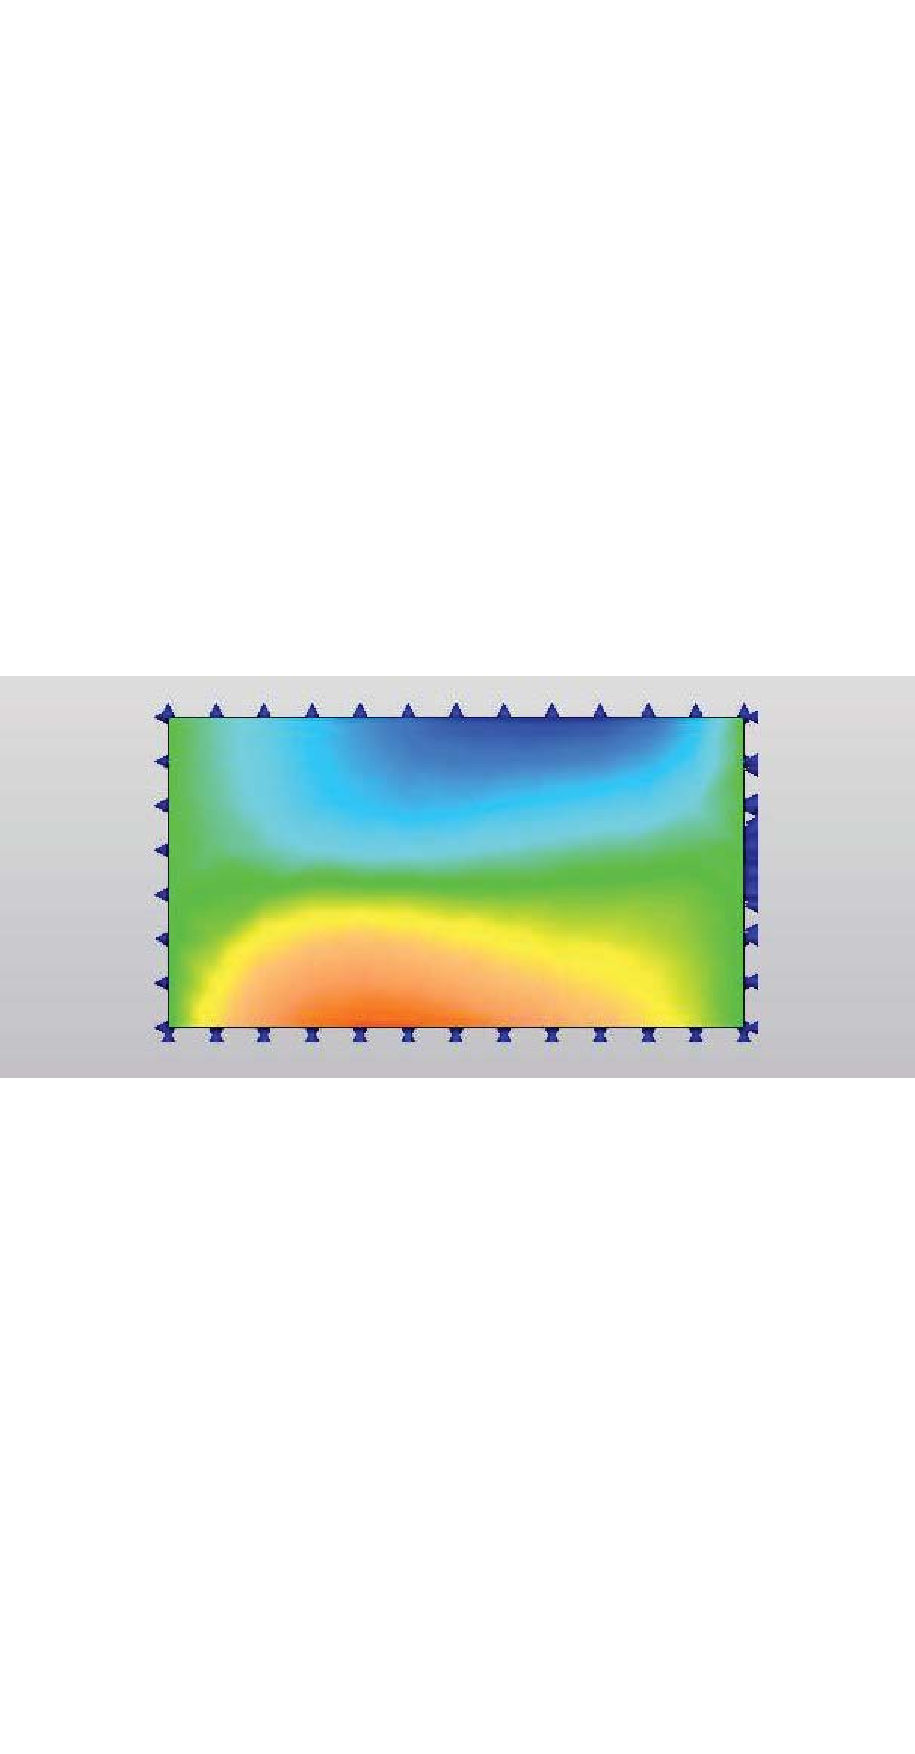
\includegraphics[]{obrazky/simulace/simulace1p}
	\caption{Zde je vidět projev víru – červená barva znázorňuje pohyb vzduchu doleva, modrá doprava. Zelená barva značí nulovou rychlost.}
	\label{sim:1}
\end{figure}
\begin{figure}[H]
		\centering
		\subfigure[Velikosti rychlosti]{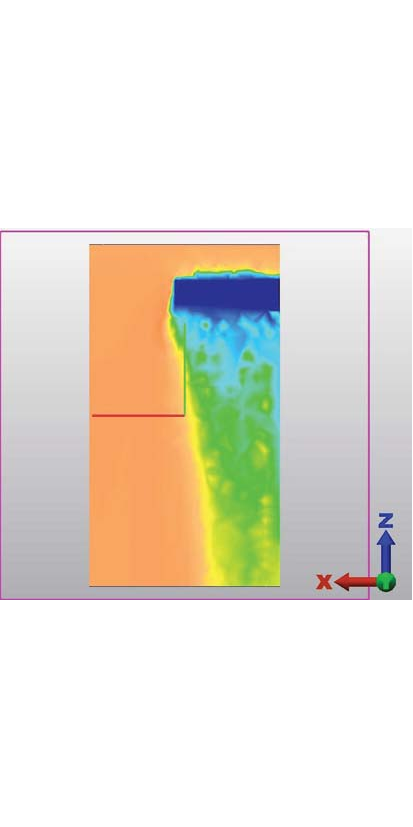
\includegraphics[]{obrazky/simulace/simulace2p}\label{sim:2}}~
		\subfigure[Velikosti rychlosti ve směru osy X]{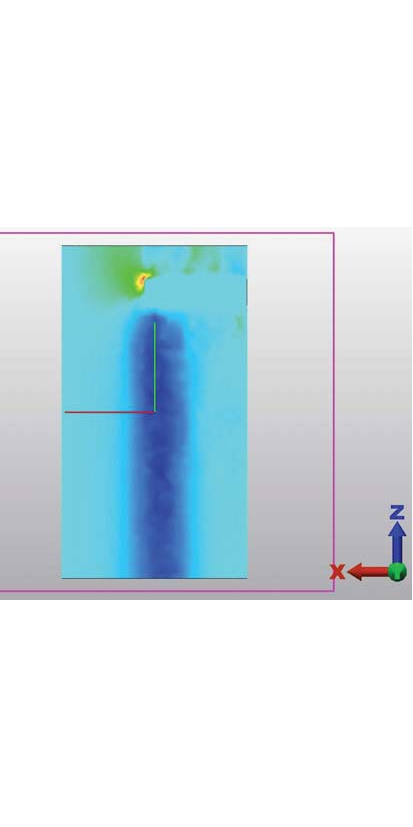
\includegraphics[]{obrazky/simulace/simulace3p}\label{sim:3}}
		\caption{Neprůkazné znázornění výsledků}
	\end{figure}


Na obrázku \ref{sim:4} jsou zobrazeny výsledky simulace listu bez jakéhokoliv zakončení. Z proudnic na tomto obrázku lze jasně vypozorovat vír, který vzniká za listem. Jelikož se proudnice při pohledu zezadu jeví dlouhé, pohybuje se vír velkou úhlovou rychlostí.

Při podrobnějším zkoumání jsem si všiml, že víru jsou dva – velký na tlakové straně a menší na podtlakové. Velký vír také zasahuje více do oblasti samotného listu, naopak malý vír se nachází až za okrajem listu. Průměr velkého víru se pohybuje mezi 20–25~cm. Malý vír má průměr menší než 10~cm. Na proudnicích lze také vidět jasný tok vzduchu mezi tlakovou a~podtlakovou stanou.

Při pohledu shora si můžeme všimnout, že vír nejznatelněji ovlivňuje posledních 15~cm listu. Na opačnou stranu je koncem listu ovlivněn i vzduch 6~cm vzdálený od konce listu.

\begin{figure}[H]
	\centering
	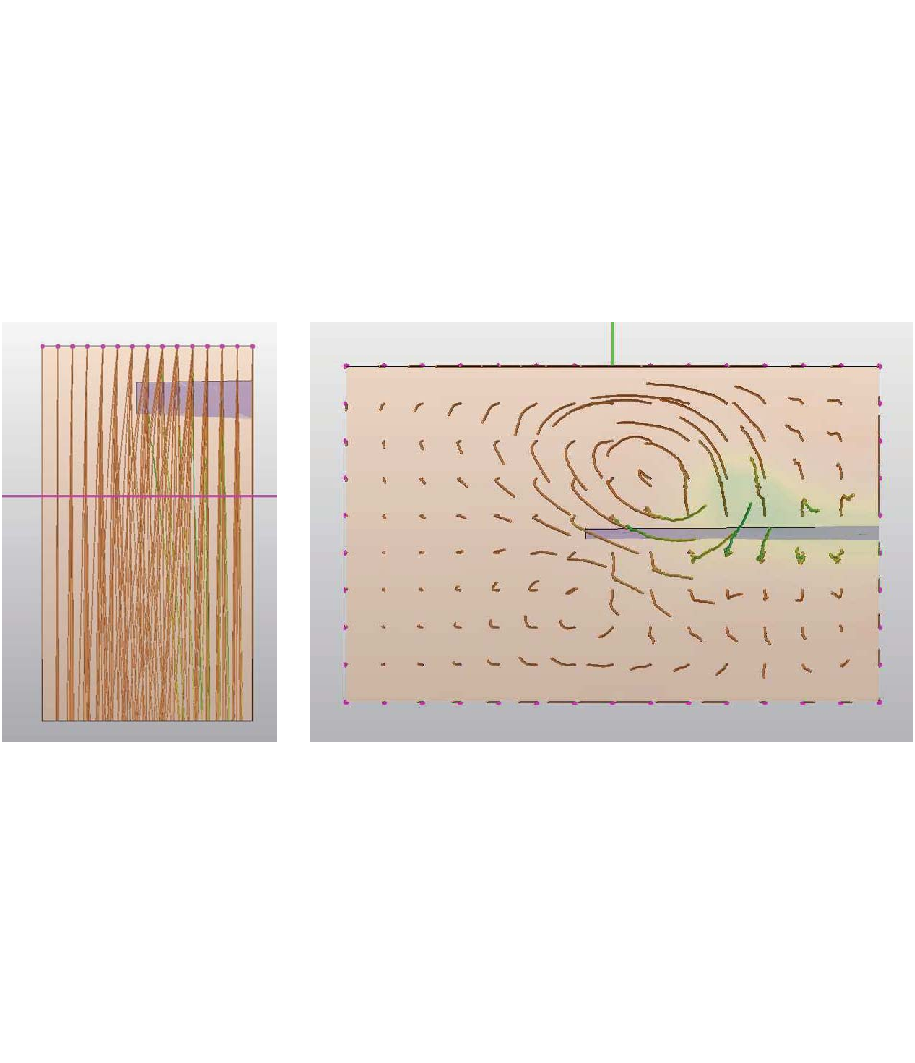
\includegraphics[]{obrazky/simulace/simulace4p}
	\caption{Proudnice listu bez zakončení. Na obrázku vpravo je jasně patrný vír za listem. Na obrázku vlevo lze vidět, jak na konci listu přestávají být proudnice rovnoběžné.}
	\label{sim:4}
\end{figure}

\subsection{Zakončení odsazením}
Autor knihy \cite{Crome:Technika} používá na svých turbínách pro snížení indukovaného odporu přesah na konci listu. Tento přesah, respektive odsazení, má za cíl omezit, popř. i úplně zamezit, toku vzduchu mezi tlakovou a podtlakovou stranou. Toto odsazení má velikost 10 mm, avšak autor má na svém listu mnohem delší tětivu než já. Rozhodl jsem se proto nasimulovat dvě velikosti odsazení – 5 a 10~mm.

Na obrázku \ref{konec:1} si lze prohlédnout model pětimilimetrového odsazení, na kterém byla provedena simulace.
\begin{figure}[H]
	\centering
	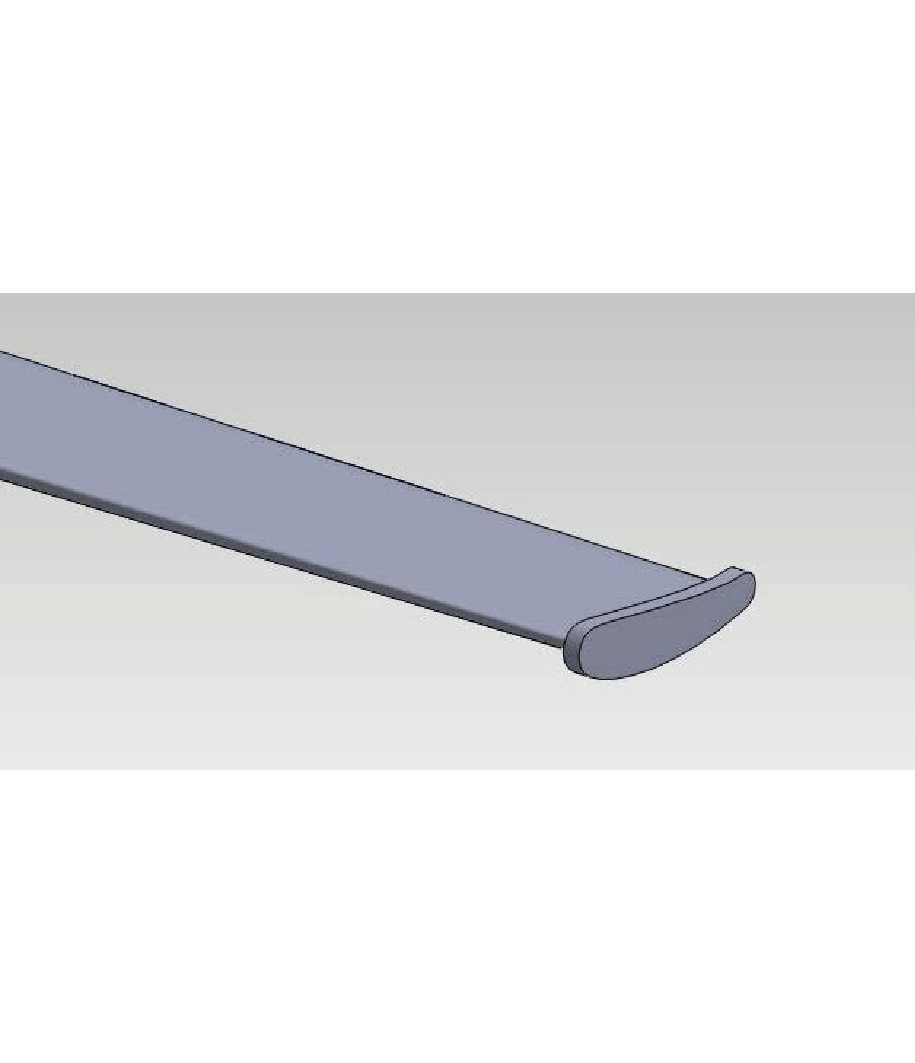
\includegraphics[]{obrazky/simulace/konec1p}
	\caption{Pětimilimetrové odsazení na konci listu}
	\label{konec:1}
\end{figure}

\begin{figure}[H]
	\centering
	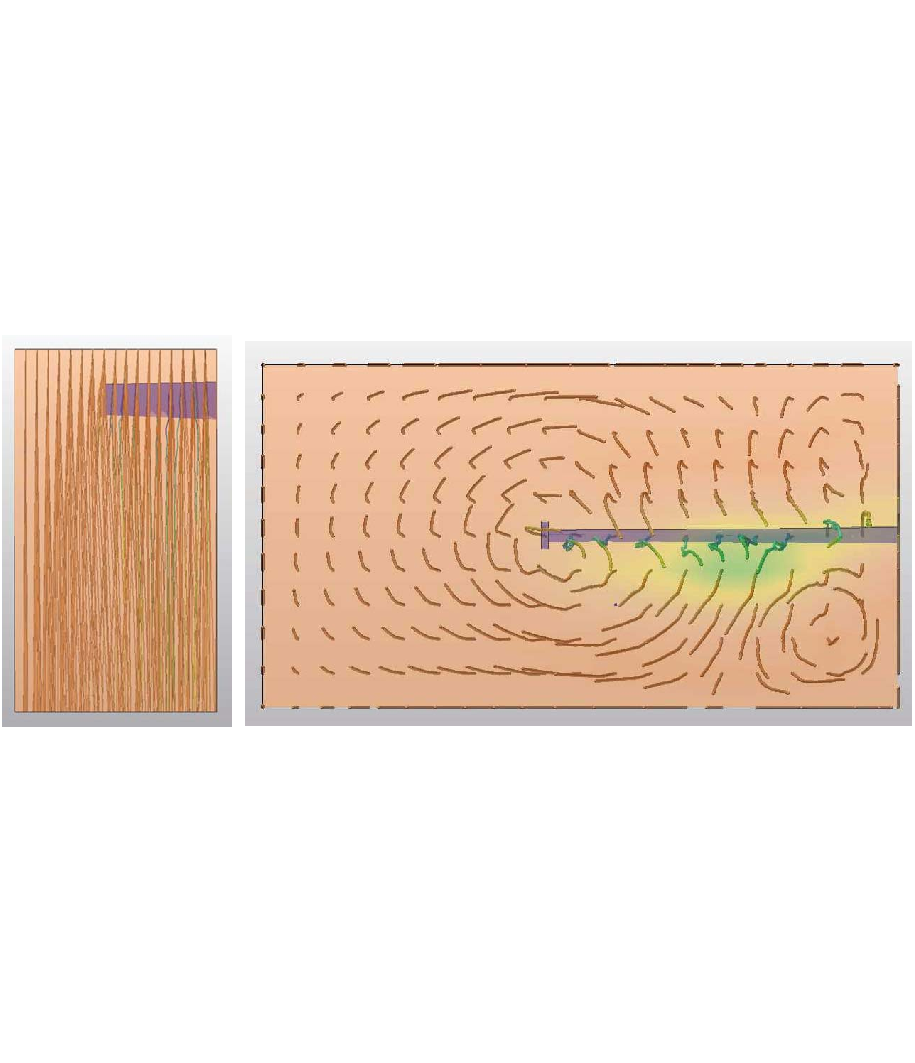
\includegraphics[]{obrazky/simulace/simulace5p}
	\caption{Výsledky pětimilimetrového odsazení na konci listu}
	\label{sim:5}
\end{figure}
Přidání této malé plošky výrazně mění charakter vnikajícího víru, jak je patrné na obrázku \ref{sim:5}. Je vidět, že vzniká pouze jediný vír, není zde přímý tok vzduchu mezi tlakovou a podtlakovou stranou a~úhlová rychlost víru je mnohem menší než v~předchozím případě. Vír se také posunul směrem z~plochy listu a~méně ji ovlivňuje.

Vír, který vzniká v pravém dolním rohu simulace, je způsoben malým simulačním prostorem – proud vzduchu zde ovlivňují stěny.
Při pohledu shora je jasně patrné minimální zakřivení proudnic. Vír tedy velmi rychle zaniká – to je dáno nižší úhlovou rychlostí.

Jinak však vypadá situace pro desetimilimetrové odsazení (obrázek \ref{sim:6}). Zde vzniká v místě zakončení proud s velkou úhlovou rychlostí obklopen druhým proudem s nízkou rychlostí. Při trojrozměrném zobrazení je vidět, že tento pomalý vír velmi rychle zaniká, avšak vnitřní vír pokračuje dále.

\begin{figure}[H]
	\centering
	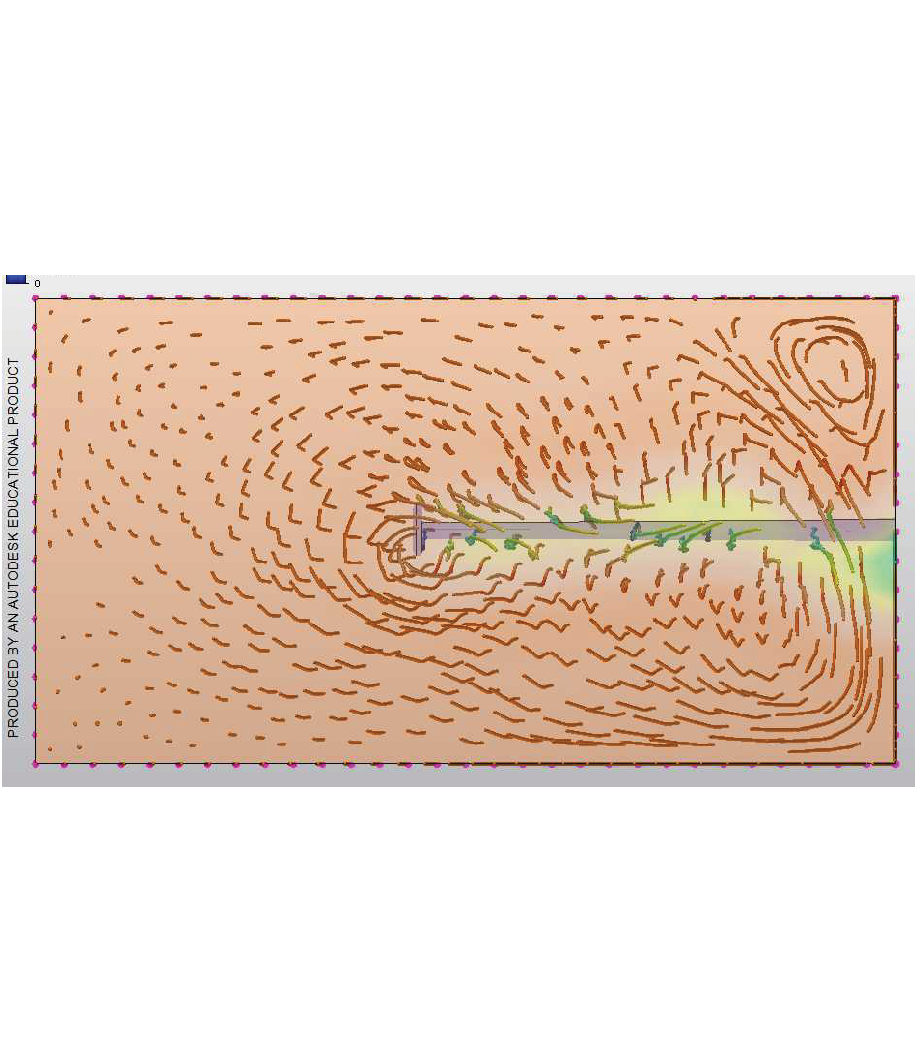
\includegraphics[]{obrazky/simulace/simulace6p}
	\caption{Výsledky desetimilimetrového odsazení na konci listu}
	\label{sim:6}
\end{figure}

Můj původní předpoklad, že délku velikost odsazení je nutno přizpůsobit délce tětivy, se ukázal jako správný. Simulace ukazuje, že pětimilimetrové odsazení pravděpodobně funguje. Díky víru s malou úhlovou rychlostí vznikají nízké ztráty a díky absenci oblasti, kde přetéká vzduch z~tlakové strany na podtlakovou, omezuje vznik hluku. Navíc výroba odsazení není technicky náročná.

\subsection{Zakončení wingletem}
Winglet je zahnutý konec křídla u letadla. Funguje na podobném principu jako odsazení – brání vzduchu proti přetékání mezi stranami aerodynamického profilu. Tím, že je však tvořen aerodynamickým profilem, vyvolává dodatečný vztlak. Poprvé byl v~praxi použit na letadle NASA \cite{winglet}.

Při použití wingletu jsem vycházel z toho, že list rotoru je jednak podobný křídlu letadla, ale také z toho, že na některých velkých větrných elektrárnách je použit. Lze ho najít také na některých typech lodních šroubů.

Bohužel jsem nenašel žádnou literaturu, která by se přímo návrhem wingletu dostatečně zabývala. Jeho tvar jsem sestavil na základě fotografií některých křídel letadel a velkých větrných elektráren. Avšak takovéto sestavení je značně nedostatečné.

Sestavil jsem 2 modely (obrázek~\ref{konec:2}) - jeden winglet zahnutý o $85\,^{\circ}$ a druhý o $65\,^{\circ}$. Winglet jsem nasměroval na podtlakovou stranu jako u křídla letadla. Winglet má stejný profil jako celý list. Délka tětivy se lineárně zmenšuje až na polovinu původní délky.

\begin{figure}[H]
	\centering
	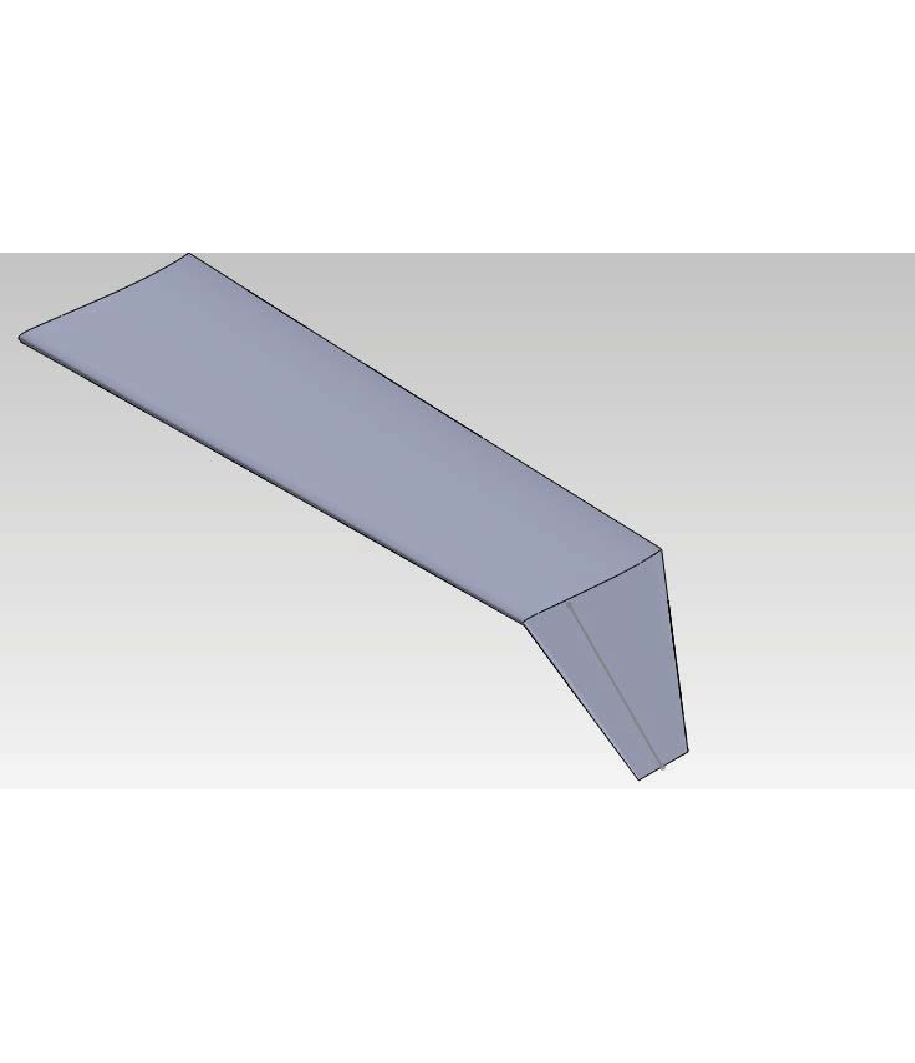
\includegraphics[]{obrazky/simulace/konec2p}
	\caption{Model wingletu}
	\label{konec:2}
\end{figure}
Od takto sestaveného modelu jsem nečekal žádné zázračné výsledky. Avšak výsledky mě překvapily – díky wingletu se odklonem $65\,^{\circ}$ vznikal za rotorem vír velkého průměru s velkou úhlovou rychlostí (obrázek \ref{sim:7}). Winglet dokonce silně ovlivňoval proud kolem celé délky simulované části profilu.

Winglet s odklonem $85\,^{\circ}$ vykazoval mnohem lepší výsledky (obrázek \ref{sim:8}) – vznikal téměř neznatelný vír s malou oblastí rychlého proudění vzduchu.

\begin{figure}[H]
	\centering
	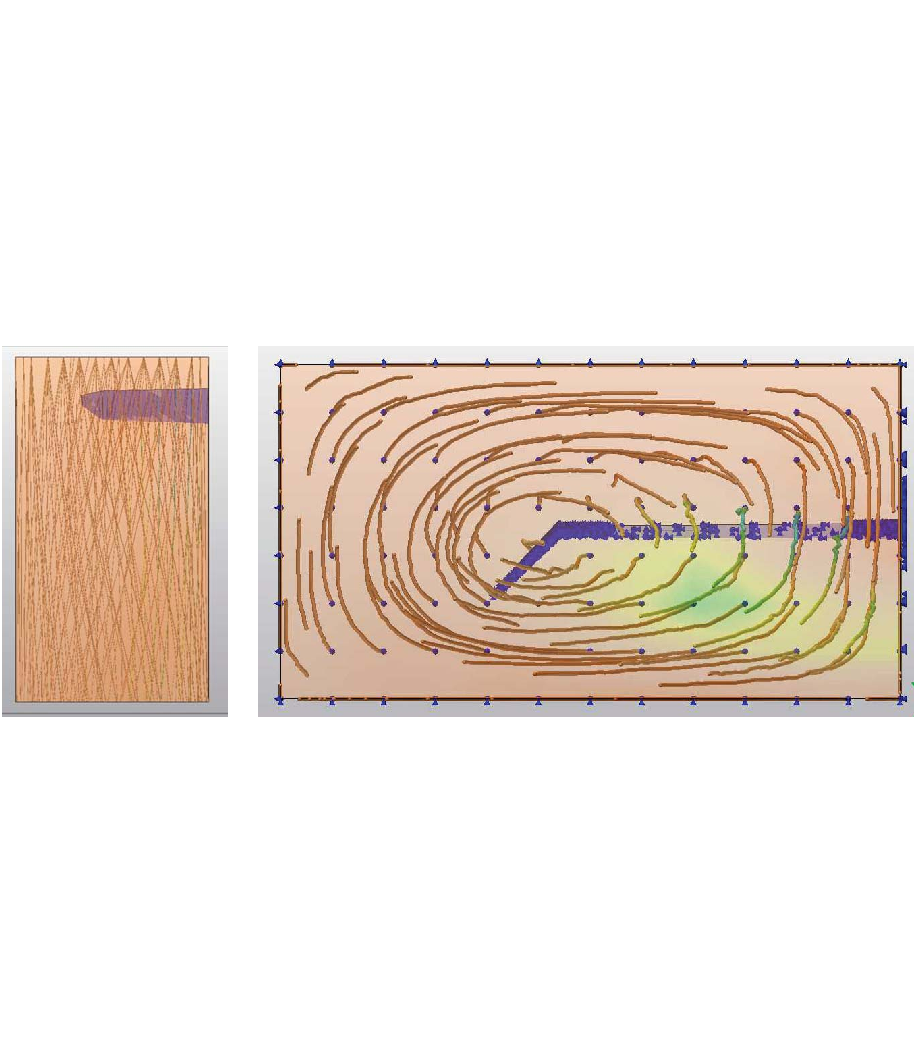
\includegraphics[]{obrazky/simulace/simulace7p}
	\caption{Simulce wingletu s odklonem $65\,^{\circ}$. Je vidět velký vír s velkou úhlovou rychlostí.}
	\label{sim:7}
\end{figure}

\begin{figure}[H]
	\centering
	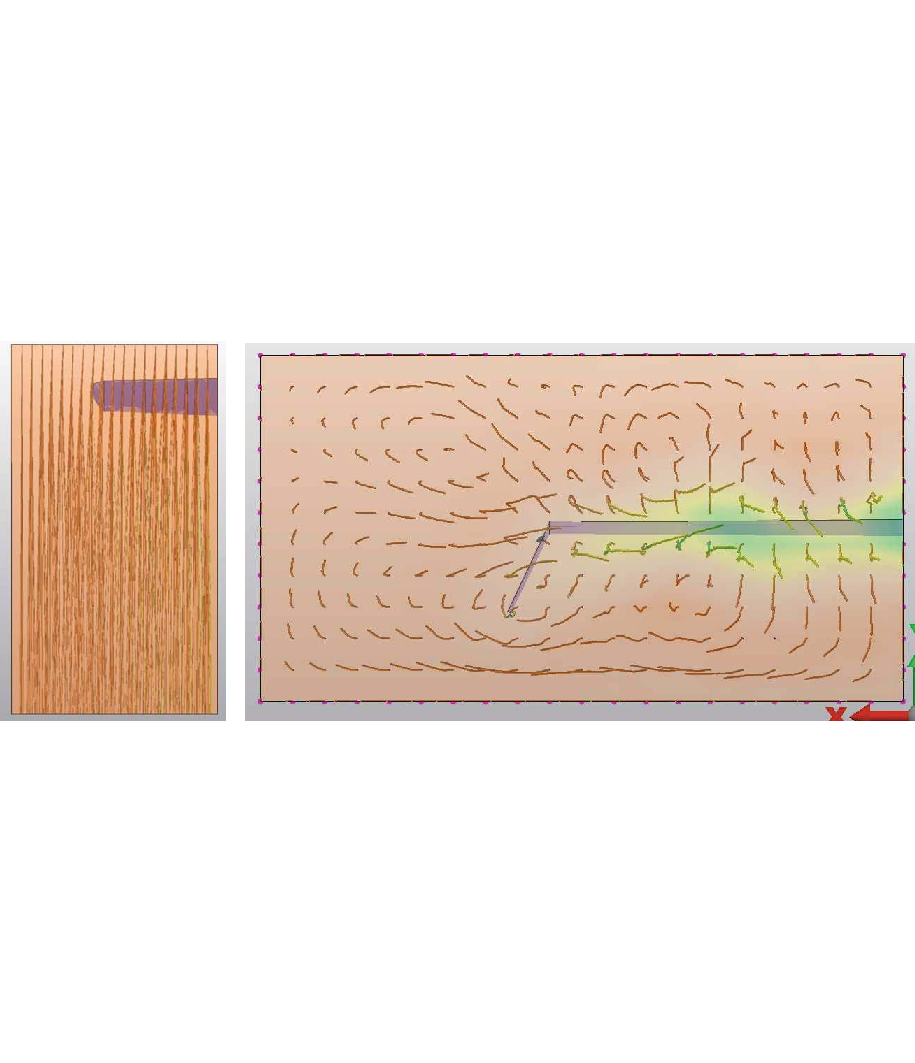
\includegraphics[]{obrazky/simulace/simulace8p}
	\caption{Simulace wingletu s odkolonem $85\,^{\circ}$. Tento wingletu vykazuje znatelně lepší výsledky než předchozí.}
	\label{sim:8}
\end{figure}
Tato simulace mě přesvědčila, že winglet je účinným řešením indukovaných ztrát, avšak také ukázala, jak choulostivá oblast zakončení listu je. I malá změna může výrazně omezit vznikající indukovaný vír, ale také jej může výrazně podpořit.

Ačkoliv jeden z mých modelů vykazoval dobré vlastnosti, rozhodl jsem se v tomto návrhu větrné turbíny winglety nepoužít. Jedná se o oblast s nejistými výsledky, které nemám nějak podložené. Avšak studium a experimenty s winglety neopouštím – rozhodně se nejedná o slepou uličku. Pouze je metoda pokusu a omylu značně neefektivní.

\subsection{Zakončení obloukem dozadu}

Na obrázku \ref{konec:3} se nachází zakončení listu obloukem dozadu. Jako inspiraci jsem si zde vzal zakončení křídel rychlostní RC modelů letadel. Toto zakončení se také často objevuje na koncích vrtulí letadel čí lodních šroubů určených pro velké rychlosti.

\begin{figure}[H]
	\centering
	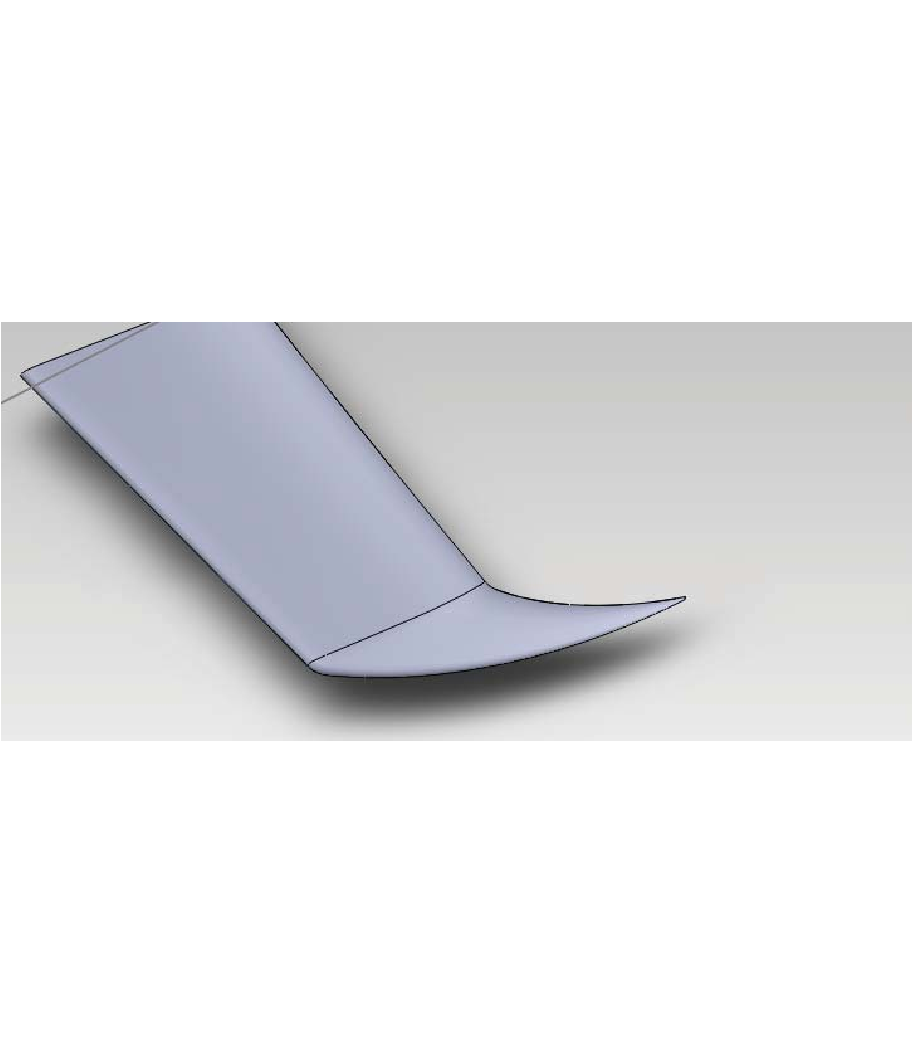
\includegraphics[]{obrazky/simulace/konec3p}
	\caption{Zakončení listu obloukem dozadu}
	\label{konec:3}
\end{figure}

Je důležité poznamenat, že tento oblouk je v rovině listu – není zahnutý. Bohužel však opět tento tvar nemám podložený teorií. I většina autorů výše uvedených modelů tvoří tato zakončení \uv{jen tak}.

Toto zakončení vytváří velký, ale relativně pomalý vír (obrázek \ref{sim:9}). Tento vír má podobné vlastnosti jako vír v případě odsazení. Na výsledcích simulace je vidět zrychlení víru, které je ovšem opět způsobeno působením stěn simulačního prostoru.

\begin{figure}[H]
	\centering
	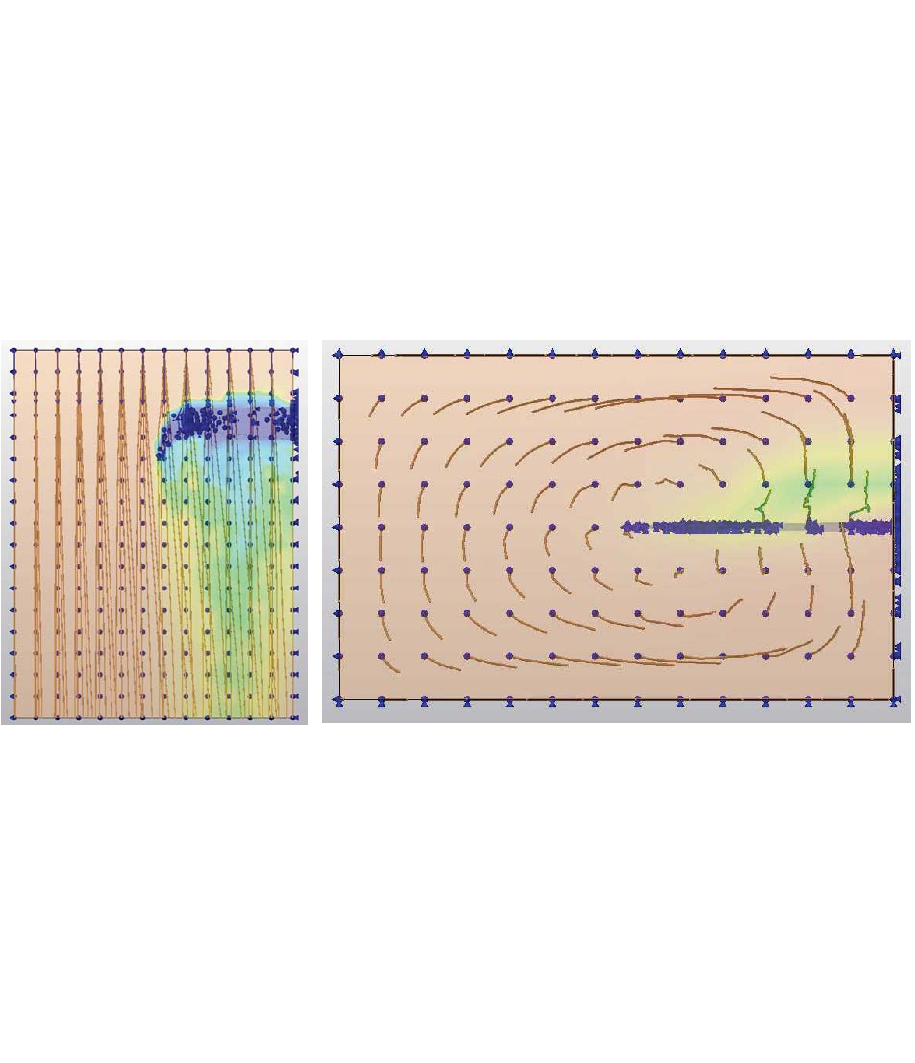
\includegraphics[]{obrazky/simulace/simulace9p}
	\caption{Výsledky simulace zakončení obloukem dozadu}
	\label{sim:9}
\end{figure}

\subsection{Zakončení kopulí}
Na spoustě malých větrných elektráren lze vidět zakončení listu kopulí. Toto zakončení je často používáno i na křídlech letadel. Model zakončení kopulí je na obrázku \ref{konec:4}.

\begin{figure}[H]
	\centering
	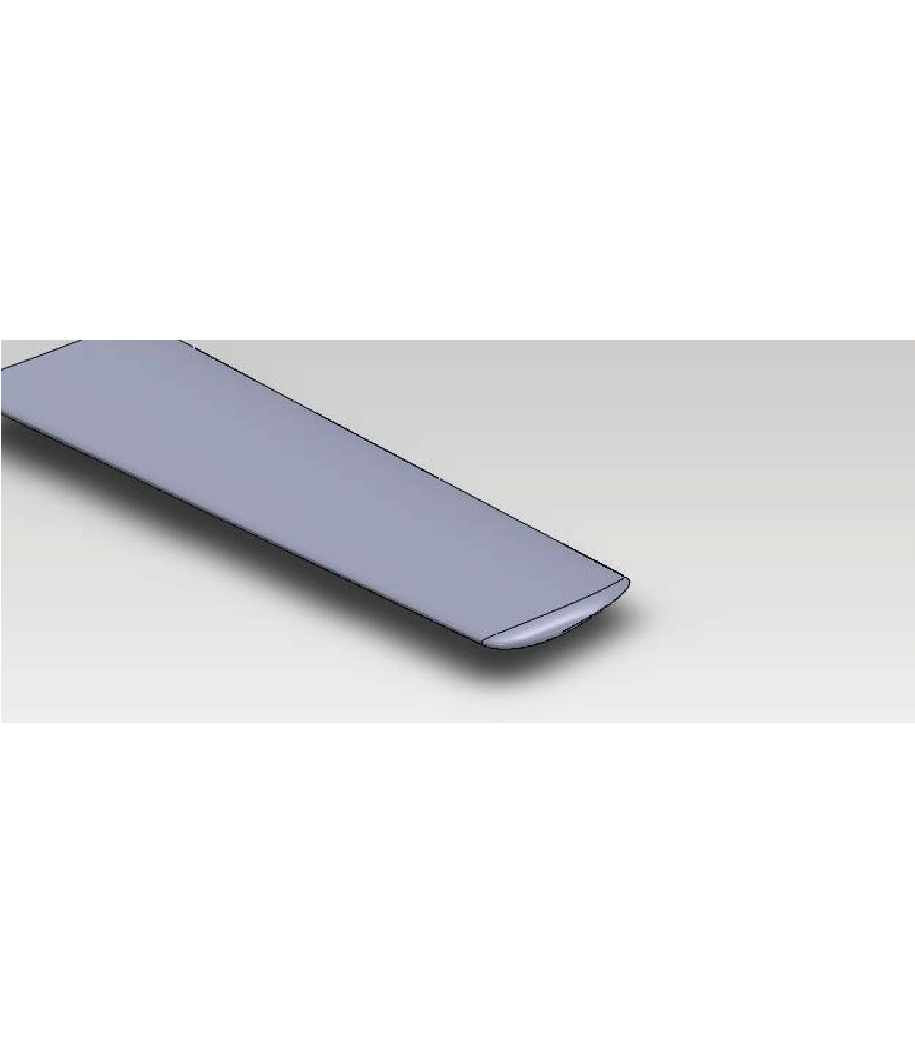
\includegraphics[]{obrazky/simulace/konec4p}
	\caption{Model zakončení listu obloukem}
	\label{konec:4}
\end{figure}

Od tohoto zakončení jsem očekával dobré výsledky – přece jen je hojně používané. Výsledky mě překvapily (obrázek~\ref{sim:10}). Na konci křídla vzniká velký vír s velkou úhlovou rychlostí. Pozitivem je, že tento vír nevzniká za aktivní plochou listu, tudíž jej příliš neovlivňuje.

\begin{figure}[H]
	\centering
	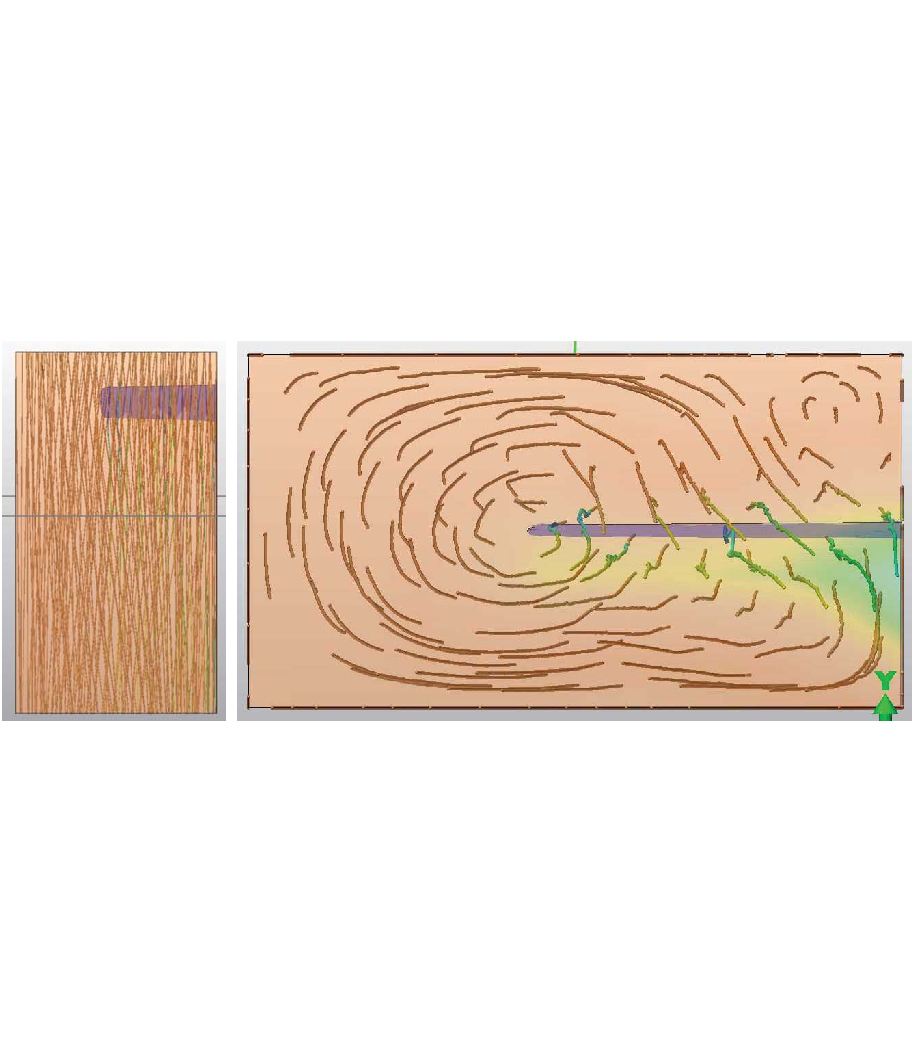
\includegraphics[]{obrazky/simulace/simulace10p}
	\caption{Výsledky simulace zakončení kopulí}
	\label{sim:10}
\end{figure}

Je však možné, že výhoda tohoto zakončení spočívá jinde. Díky tomu, že tečně navazuje na konec listu a jedná se o hladkou plochu bez ostrých hran, nevznikají na tomto zakončení chvění vzduchu způsobující hluk. Tuto domněnku však nemohu potvrdit – simulaci tohoto typu jsem nebyl schopen provést.

\subsection{Výběr zakončení}
Z výše uvedeného porovnání vyplývá, že dobré výsledky dává zakončení pětimilimetrovým odsazením, wingletem a obloukem dozadu.

Pro svůj model jsem použil odsazení, jelikož se jedná o tvar, ve kterém hraje roli jediná proměnná – velikost odsazení a ta jde jednoduše nasimulovat. Ostatní zakončení jsou komplexními tvary, které za některých okolností podávají dobré a za některých okolností špatné vlastnosti.

	\chapter{Výsledek návrhu}
V této kapitole si můžete prohlédnout obrázky výsledného tvaru turbíny. Na model byl přidán náboj s parabolickým tvarem. Jeho cílem je chránit nosnou konstrukci před povětrnostními podmínkami a vytvořit kolem nich aerodynamický obal. Náboj má průměr 25 cm. Na jeho úkor byl zkrácen list o oblast, která podává minimální výkon. List přímo navazuje na náboj. Jakékoliv složitější navázání zde nemá smysl řešit díky malé rychlosti proudícího vzduchu. Provedené změny (obrázky \ref{cel:1} až \ref{cel:3}) můžete porovnat s obrázky \ref{obr.model1} až \ref{obr.model3}.
\begin{figure}[H]
	\centering
	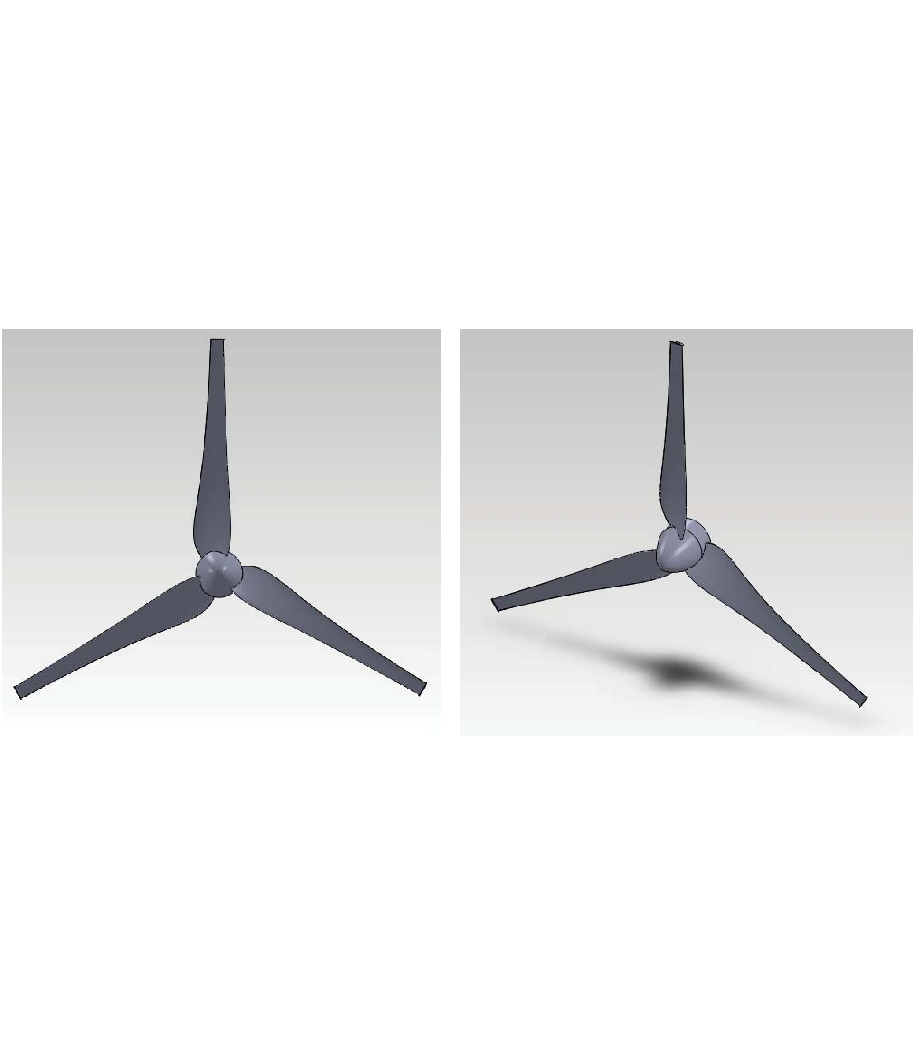
\includegraphics[]{obrazky/celek1}
	\caption{Pohled na celou turbínu}
	\label{cel:1}
\end{figure}
\begin{figure}[H]
	\centering
	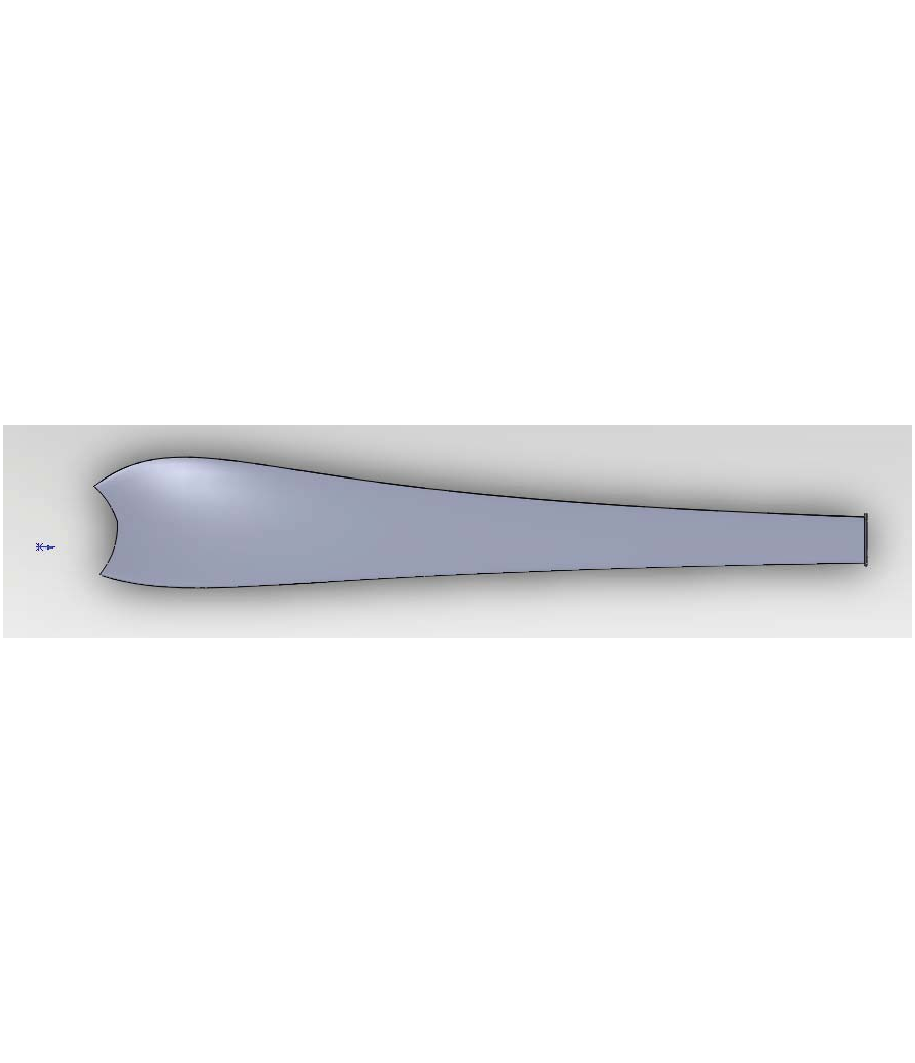
\includegraphics[]{obrazky/celek3}
	\caption{Celkový pohled na list. Modrý bod označuje osu otáčení.}
	\label{cel:2}
\end{figure}
\begin{figure}[H]
	\centering
	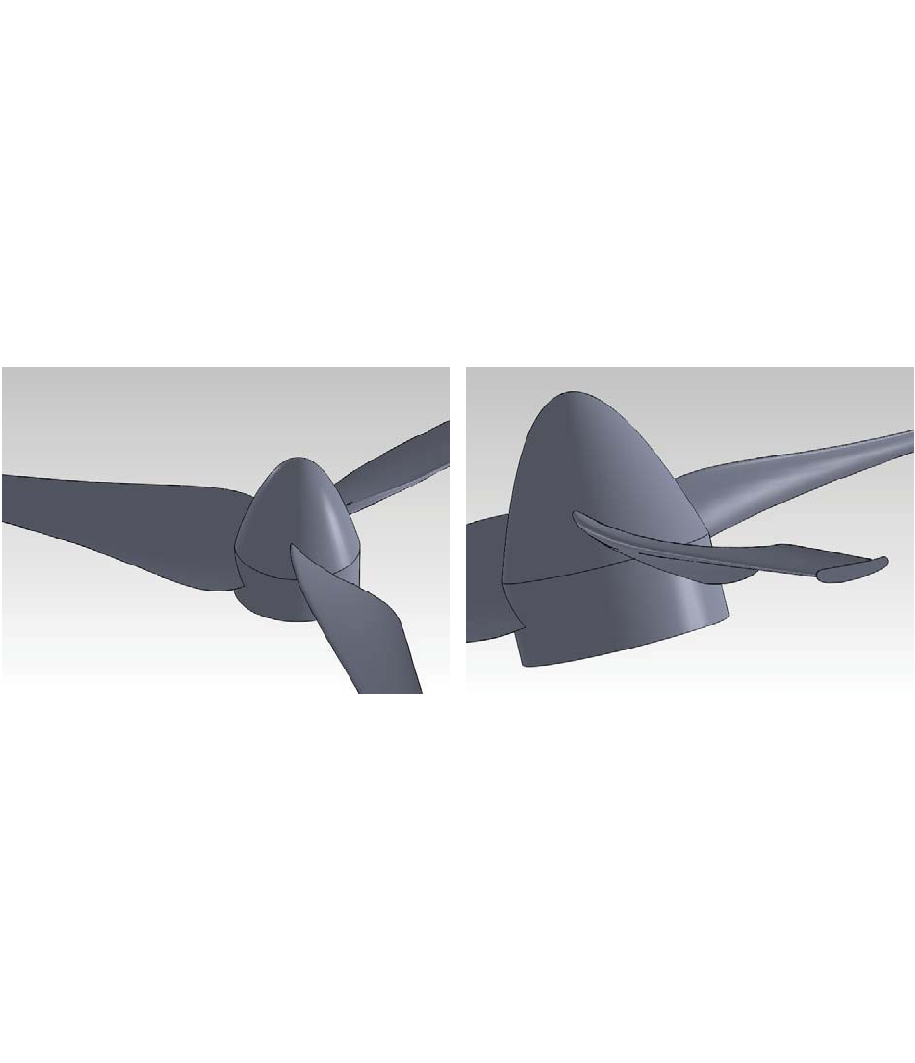
\includegraphics[]{obrazky/celek2}
	\caption{Detail navázání listu na náboj a zakončení listu odsazením}
	\label{cel:3}
\end{figure}

	\part{Stavba a zkušenosti s~provozem prvního prototypu}\label{part:stavba}
		\chapter{Návrh prvního protoypu}
V této kapitole popisuji návrh prvního prototypu. Tento prototyp byl první realizovanou turbínou, a proto na ní lze najít spoustu i zásadních chyb. I přes to byla stavba této turbíny velkou a neocenitelnou zkušeností.

První prototyp byl navržen pomocí zjednodušené teorie. Hlavním zdrojem informací tehdy byly internetové stránky \cite{ve:ve}. 

Jelikož se jednalo o první turbínu, byl záměrně zvolen hodně malý průměr – 1,5~m. Tento průměr se ukázal pro první pokusy jako ideální. Dobře se s touto velikostí pracuje. Při údržbě není s trochou opatrnosti problém manipulovat se složenou turbínou i v interiéru.

\begin{figure}[H]
	\centering
	\includegraphics[]{obrazky/prot1p}
	\caption{Pohled na celý CAD model prvního prototypu}
	\label{prot1}
\end{figure}

\begin{figure}[H]
	\centering
	\includegraphics[]{obrazky/prot2p}
	\caption{Pohled na list prvního prototypu}
	\label{prot2}
\end{figure}


Byla také zvolena nízká rychloběžnost turbíny kvůli obavám z hluku. Ty se ukázaly po více než ročním provozu jako neopodstatněné. Nízká rychloběžnost však přinesla jeden neočekávaný negativní efekt. Při nižší rychlosti větru se i turbína otáčí relativně pomalu a vrhá mihotavý stín, který může působit rušivě. Při silnějším větru se však stín přestává mihotat a jeví se jako polostín. Z tohoto důvodu byla při novém návrhu turbíny použita rychloběžnost 5.


Byl použit profil SG6043. Profil byl vybrán hlavně díky jeho vzhledu a jemnosti. Nebyl dále nějak zkoumán. Shodou okolností se později ukázalo, že tento profil je pro použití na větrné turbíně velmi vhodný.

Pro výpočet byl list rozdělen na 7 částí. U osy otáčení byly použity 4 části s tloušťkou 3 cm, jelikož blízko osy otáčení je změna délky tětivy a úhlu náběhu velká. Naopak ke konci listu se tyto změny snižují, a proto byly použity části s~tloušťkou 9, 12 a 15~cm. Pro každou tuto část byl vypočten úhel náběhu a délka tětivy. Následně byly tyto průřezy lineárně spojeny. Na základě těchto dat jsem vytvořil CAD model složený z jednotlivých částí (obrázek \ref{prot1}).

Listy byly zakončeny malým obloukem. Pro navázání na náboj byla přidána jedna část o~tloušťce 1~cm, která má stejnou délku tětivy i úhel náběhu jako předchozí. Na ni navazuje třícentimetrová část, která se sbíhá do kruhu o průměru 2 cm.

Na obrázcích CAD modelu (\ref{prot1} a \ref{prot2}) si lze všimnout největší chyby v návrhu, která v~podstatě znemožnila použití této turbíny pro zisk energie. Je prohozená tlaková a podtlaková strana profilu. Při návrhu jsem se příliš inspiroval klasickými leteckými vrtulemi, které fungují přesně naopak – proud vzduchu urychlují, nikoliv jej zpomalují.

Tato chyba výrazně snižuje podávaný výkon a účinnost této turbíny. Avšak díky použitému profilu neznemožnila zcela funkci turbíny. Při pohledu na graf průběhu součinitele vztlaku v~závislosti na úhlu náběhu (graf \ref{graf:zavislost1}) lze zjistit, že při neoptimálním úhlu náběhu $-5\,^{\circ}$ profil SG6043 stále dosahuje kladné hodnoty součinitele vztlaku. Konkrétně hodnoty 0,36. Součinitel odporu při tomto úhlu náběhu nepatrně vzrostl. Hodnota součinitele vztlaku je $3,5\times$ nižší. Díky tomu turbína dosahuje minimálního výkonu. 






\chapter{Výroba prvního prototypu}
\section{Výroba listů}
V této kapitole popisuji postup a technologii výroby, kterou byly vytvořeny listy prvního prototypu. Dále shrnuji výhody a nevýhody použitého postupu.

Pro výrobu listu bylo nutné zvážit několik požadavků. Prvně je nutné nějakým způsobem dodržet správný tvar. List by měl být vyroben z materiálu, který se dá snadno opracovat a měl by být zvolen postup, kterým jdou vyrobit 3 listy s co nejmenšími odchylkami v jejich tvaru. Dále by měl být použitý materiál co nejlehčí, aby nebyl náboj příliš zatěžován odstředivou silou. List však musí vydržet odpor větru.

Listy jsou vyrobeny ze zbytků zateplovacího polystyrenu. Uvnitř nich je nosná konstrukce složená z ocelové tyče o průměru 10 mm a délce 240 mm (z toho 160 se nachází uvnitř listu). Na tuto kulatinu byla připájena tenčí, pětimilimetrová, kulatina o délce 360 mm, která tvoří výztuhu u konce listu, kde je profil tak tenký, že se zde desetimilimetrová kulatina nevleze. Povrch listů je potažen dvěma vrstvami netkané textilie prosycené lepidlem.

Jednotlivé části listu byly vyříznuty nažhavený drátem (odporový drát připojený na zdroj stejnosměrného proudu) podle připravených šablon z hliníkového plechu. Tyto šablony byly vytvořeny z výše uvedeného CAD modelu. Jejich tvar byl vytištěn na laserové tiskárně a následně přežehlen na hliníkový plech. Tyto šablony pak byly vyříznuty a dobroušeny na požadovaný tvar.

Výroba každé části listu probíhala následovně. Prvně jsem uřízl nažhaveným drátem desku polystyrenu požadované tloušťky. Do ní jsem následně vyvrtal trubkovým vrtákem díru pro nosník. Do díry jsem nasadil pomocný kolík a pomocí něj přilepil oboustrannou lepicí páskou jednu šablonu. Na druhou stranu byla přilepena adekvátní šablona. Jejich vzájemnou pozici určoval kolík v díře pro nosník a pak dále značky vytvořené v CAD modelu. Tyto značky musí s kolíkem ležet v jedné rovině. Tím bylo zajištěno správné zkroucení dané části.

Samotné vyříznutí podle šablon vyžadovalo trochu nácviku a zkoušení. Prvně bylo nutné najít správný proud, který musí drátem téci, aby polystyren řezal, ale nepálil. Dále bylo nutné se naučit, jak drátem táhnout. Problém zde byl v tom, že šablony mají různou velikost a rozdílný obvod. Na jedné straně je tedy nutné drátem táhnout rychleji. To se mi po určitém nácviku nakonec povedlo a~byl jsem schopen řezat bezchybné tvary. Na závěr byly šablony odlepeny pomocí několika kapek technického benzínu, který rozpustil lepidlo lepicí pásky.

Jednotlivé části potom byly slepeny pomocí lepidla UHU por. Části se k sobě lepily nasazené na nosníku, čímž byla zajištěna jejich správná pozice. List byl po slepení přilepen k nosníku. Prvně pomocí lepidla UHU por, to se však ukázalo jako nespolehlivé pro spojení polystyrenu a~kovu. Po několika dnech provozu turbíny jeden z listů vlivem odstředivé síly upadl. Na nosníky proto byla vybroušena plytká drážka ve tvaru spirály a listy byly přilepeny lepidlem Purex. Toto lepidlo při tvrdnutí pění a vyplňuje velký prostor. Proto zateče mezi jednotlivé kuličky polystyrenu a zároveň do drážky na nosníku. Tento spoj se ukázal jako spolehlivý – již přes rok pevně drží.

List byl postupně potažen dvěma vrstvami netkané textilie prosycené lepidlem Herkules. Tato povrchová skořepina dodala listu pevnost a odolnost vůči povětrnostním podmínkám. Původně měl být list ještě natřen epoxidovým lakem pro zvýšení odolnosti. Avšak ani 2 vrstvy netkané textile nejsou dokonale nepropustné a lak se na pokusném listu prosákl dovnitř a rozpustil polystyren. Jak ukázal čas, listy jsou i bez tohoto nátěru dostatečně odolné. List byl na závěr natřen třemi vrstvami bílého latexového nátěru.

Pro statické vyvážení celého rotoru bylo nutné dva listy dovážit olověnými závažíčky o hmotnosti 2 a 1 gram. Tato závažíčka byla přilepena vteřinovým lepidlem. K mému překvapení i po roce provozu stále drží přilepená.

\section{Umístění - gondola, stožár}
Jelikož jediné možné umístění turbíny je na zahrádce, vznikl požadavek na stožár – nesmí mít kotvící lana. Na stožár byl použit 3,5 m dlouhý starý anténní stožár. Pro případnou demontáž není přímo ukotven v zemi.

Do hloubky 1 m byla zabetonována 2 m dlouhá trubka, která slouží jako lože pro stožár. V~případě potřeby je možné tedy stožár z této ukotvené trubky vysunout a schovat. Stožár je v~této trubce jištěn 6 šrouby zašroubovanými do navařených matek. Celé toto kotvení se v~průběhu času ukázalo jako spolehlivé – i při nejvyšší vichřici netrpí základy stožáru nějakými vibracemi.

Gondola, na níž je umístěna turbína, vznikla svařením dvou vinklů k sobě pomocí kolmých kousků pásoviny. Na její spodní stranu bylo přivařeno svislé ložisko, okolo kterého se celá gondola otáčí. Jako ložisko pro samotnou turbínu byl použit starý stejnosměrný elektromotor. Ten byl vložen do gondoly a přitažen kovovými stahovacími páskami. Kormidlo, které řídí natáčení celé gondoly, bylo vyříznuto za plastové desky.

Náboj rotoru byl vytočen z kusu hliníku. Do něj byly vyvrtány díry pro nosníky listů. Na nosníky listů byly vyfrézovány plošky, za které je nosník v náboji přitažen.

Na tento samotný náboj jsem vytvořil ještě kryt. Tento kryt není důležitý z aerodynamického hlediska (u takto malé plochy je jeho přínos minimální), ale má hlavně funkci estetickou a chrání náboj před povětrnostními vlivy. Tento náboj byl vytvořen stejnou technologií jako listy. Vytvořil jsem si 2 šablony z hliníkového plechu. Odporovým drátem jsem si nařezal $30^{\circ}$ výseče. Na tuto výseč jsem nalepil šablony a podle šablony jsem vyřízl část náboje. Následně jsem slepil 12 takto vyříznutých výsečí do plného kruhu. Tím vznikl základní tvar náboje, do kterého jsem ještě vyvrtal otvory pro nosníky listů a otvory pro utažení šroubů. Náboj nebyl potažen netkanou textilií – jeho tvar by se špatně potahoval. Byl pouze natřen latexovým nátěrem. Po roce provozu se nátěr začal mírně loupat a na polystyrenu byla patrná deformovaná místa od UV záření.

\chapter{Zkušenosti s provozem}

První prototyp byl vyroben na přelomu září a října 2010. Stožár i s turbínou byl umístěn 29.~října. Od té doby byla turbíny nepřetržitě v provozu.

První problém nastal dva týdny po instalaci – tehdy, jak jsem zmínil výše, upadlo polystyrenové tělo z nosníku. Po změně lepidla se tento problém již znovu neobjevil.

Zhruba po půlroce se ukázalo vertikální ložisko turbíny jako nespolehlivé. Vlivem změny teplot v něm kondenzovala voda a ložisko zarezlo. Po jeho úpravě funguje spolehlivě.

Další problém se netýkal turbíny samotné, ale jejího uložení. Vlivem povětrnostních podmínek se v září 2011 odlepil jeden permanentní magnet uvnitř motoru použitého jako ložisko a začal drhnout o rotor. Motor vydával skřípavý zvuk. Jelikož však motor nelze použít jako generátor (díky nízkým otáčkám turbíny), stačilo uvolněný magnet vytáhnout.

Celá konstrukce turbíny se během roku provozu osvědčila. Původní obavy z hlučnosti se nepotvrdily. Turbína byla i při sebesilnějším větru tichá. Aby byl vůbec slyšet nějaký hluk, musel člověk stát přímo pod stožárem. Ale i tak nebyl hluk větší než např. šumění listí stromů v okolí.

Velký podíl na tomto faktu může mít použití polystyrenu jako hlavního materiálu – listy jsou díky tomu měkké, a tak nepřenáší chvění na celou konstrukci a chvění to nemůže rezonovat. Listy také nejsou křehké a vydržely i krupobití.

Turbína také vyniká svou startovatelností – může za to mohutná oblast listů blízko osy otáčení. Při prvních pokusech jsem zkoušel s turbínou chodit – i takto pomalý proud vzduchu ji zvládl roztočit.

Stožár se také ukázal jako dostatečně pevný. Jelikož je turbína relativně malá, nebyla použita žádná ochrana proti silnému větru. Při silném větru je patrné, jak se stožár na svém vrcholu lehce kýve, ale jinak nic.

Velmi mě překvapila odolnost použité povrchové úpravy. Celý nátěr vydržel bez většího poškození celý rok. V lednu 2012 jsem provedl preventivní údržbu. Turbína byla sundána a~listy byly znovu natřeny. Na původním nátěru byly místy patrné malé praskliny, u konců listů se několik šupinek odlouplo. Avšak vnější skořepina z netkané textilie nejevila žádné známky poškození.

Bohužel turbínu nešlo díky záměně tlakové a podtlakové strany připojit na generátor a získat nějakou elektrickou energii.
Za celou dobu provozu se turbína stala vyhledávanou atrakcí malých dětí. Nebyly na ni žádné negativní ohlasy.

\begin{figure}[H]
	\centering
	\includegraphics[]{obrazky/foto1}
	\caption{Sušení nově natřených listů při první údržbě v lednu 2012 (vlevo) a pohled na složený rotor (vpravo)}
	\label{foto1}
\end{figure}

\begin{figure}[H]
	\centering
	\includegraphics[]{obrazky/foto2}
	\caption{Pohled na celou gondolu}
	\label{foto2}
\end{figure}

\begin{figure}[H]
	\centering
	\includegraphics[]{obrazky/foto3}
	\caption{Pohled na stožár (vlevo), pohledy na turbíny při relativně silném větru (vpravo)}
	\label{foto3}
\end{figure}


	\part{Závěr}\label{part:zaver}
		\chapter{Zhodnocení práce}
Cílem této práce bylo seznámit čtenáře s aerodynamikou malých větrných turbín a ukázat její použití v praxi – jak při návrhu, tak i samotné stavbě. Tyto cíle se podařilo splnit.

V této práci jsem na základě Glauertovy teorie navrhl větrnou malou větrnou turbínu. Tuto teorii jsem doplnil o poznatky získané z předchozí stavby prvního prototypu a zkusil jsem na základě aerodynamických simulací optimalizovat zakončení listu větrné turbíny.

\chapter{Budoucnost projektu}

Jak je patrné z celé práce, práce na projektu malé větrné elektrárny není hotová a vyžaduje ještě spoustu času.

V budoucnu by měla být výše navržená turbína vyrobena. Technologie výroby zatím není známa. Pokud to dovolí prostředky, měly by listy být vyrobené z laminátu.

Tato turbína bude připojena na pomaloběžný generátor, jehož vývoj je téměř u konce. Momentálně se nachází ve fázi testování. Energie vyrobená touto elektrárnou by ke své povaze (nestálé frekvenci a napětí) měla být použita k dotápění domu či ohřevu vody.

K elektrárně je také nutno dodělat komplexní ochranný systém před vichřicí a dalšími vlivy. Jelikož výkon turbíny neroste s otáčkami (otáčky rostou s rychlostí větru lineárně, výkon s třetí mocninou) je nutné přidat elektronické spínání zátěže generátoru, aby byla turbína efektivně využita. Elektrárna by také měla být doplněna o čidla a vybavena telemetrií s ukládáním dat a webovým rozhraním. Tento systém telemetrie mi již částečně funguje na pokusném anemometru. Je založen na routeru Asus WL-500GP. Avšak mám v plánu tento systém přestavět na platformu ARM, konkrétně na mikroprocesory STM32 kvůli jejich minimální spotřebě, velikosti a ceně v~porovnání s routerem. Mikroprocesor se navíc lépe zabudovává do embedded systému. Elektrárna by také měla jít z webového rozhraní ovládat – např. ji odstavit z provozu.


% % % % % % % % % % % % % % % % % % % % % % % % % % % % % % % % % % % % % % % % % % % % % %



% Bibliografie
\nocite{*} % Uvést všechny záznamy, i necitované
\bibliography{00-Reference/Reference}
\addcontentsline{toc}{chapter}{Literatura}
\cleardoublepage

% Nastaví číslování stránek pro přílohy
\pagenumbering{Roman}



% Přílohy
\part{Přílohy}
\begin{appendix}
% % % % % % % % % % % % % % % % % % % % % % % % % % % % % % % % % % % % % % % % % % % % % %
% Zde se vkládají přílohy
% Můžete vkládat soubory TeX či přímo PDF soubory
% Samotný text příloh doporučuji kvůli přehlednosti mít ve zvlášních souborech
%	\chapter{Seznam použitých součástek}

Zde sepsaný seznam součástek je pouze orientační pro stavbu nové mlžné komory shodné s mnou postavenou. Na tu byly použity položky z tohoto seznamu. Ne všechny ale byly nově zakoupené, například zdroj, chladič a mnohé jiné pocházely ze starších počítačů, z mých předchozích experimentů apod. Celkové náklady na stavbu mlžné komory tedy byly mnohem menší. Uvedené ceny jsou při zakoupení nových dílů zjištěné k 2.~říjnu~2010.

\begin{table}[h]
	\centering
	\caption{Seznam součástek použitých při stavbě mlžné komory.}
	\label{tab:SeznamSoucastek:Komora}
	\begin{tabular}[t]{|r@{$\,$}l|p{4.6cm}|p{4.2cm}|p{3.1cm}|r@{$\,$}l|}
		\hline
		$ 1 $ & $\mathrm{l} $ & isopropanol												&	\href{http://www.ges.cz/-izoprop-1l-ges08000029.html}{IZOPROP 1L}																		&	\href{http://www.ges.cz}{GES Electronics}								&	$ 189 $ & $\textrm{Kč} $	\\
		$ 1 $ & $\mathrm{ks} $ & chladič 													&	\href{http://www.alza.cz/chladic-arctic-freezer-64-d56766.htm}{ARCTIC Freezer 64 PRO}									&	\href{http://www.alza.cz}{alza.cz}												&	$ 443 $ & $\textrm{Kč} $	\\
		$ 1 $ & $\mathrm{ks} $ & peltierův článek $ 51 \, \mathrm{W} $	&	\href{http://www.gme.cz/cz/m-tec1-12706-p601-017.html}{M-TEC1-12706}														&	\href{http://www.gme.cz}{GM Electronic}									&	$ 155 $ & $\textrm{Kč} $	\\	
		$ 1 $ & $\mathrm{ks} $ & peltierův článek $ 89 \, \mathrm{W} $	&	\href{http://www.gme.cz/cz/m-tec1-12710-p601-012.html}{M-TEC1-12710}														&	\href{http://www.gme.cz}{GM Electronic}									&	$ 177 $ & $\textrm{Kč} $	\\	
		$ 25 $ & $\mathrm{g} $ & teplovodivá pasta									&	\href{http://www.gme.cz/cz/pasta-teplovodiva-dc-se4490-cv-p749-069.html}{DC SE4490 CV}							&	\href{http://www.gme.cz}{GM Electronic}									&	$ 230 $ & $\textrm{Kč} $	\\	
		$ 2 $ & $\mathrm{ks} $ &LED modul												&	\href{http://www.gme.cz/cz/led-modul-vodotesny-5x-autoled-bila-78x18-mm-p960-164.html}{LED modul vodotěsný 5x autoled, bílá, 78x18 mm}			&	\href{http://www.gme.cz}{GM Electronic}			&	$ 24 $ & $\textrm{Kč} $	\\	
		$ 1 $ & $\mathrm{m} $ & odporový drát											&	\href{http://www.gme.cz/cz/rg-odp-kan01-p653-005.html}{RG-ODP-KAN01}														&	\href{http://www.gme.cz}{GM Electronic}									&	$ 22 $ & $\textrm{Kč} $	\\	
		$ 1 $ & $\mathrm{m} $ & rezistor $ 3,3 \, \mathrm{\Omega} $		&	\href{http://www.gme.cz/cz/rr-w10-3-3r-p114-186.html}{RR W10-3.3R}																	&	\href{http://www.gme.cz}{GM Electronic}									&	$ 10 $ & $\textrm{Kč} $	\\	
		$ 1 $ & $\mathrm{m} $ &smršťovací bužírka									&	\href{http://www.gme.cz/cz/f0920hs-15-bk-p656-467.html}{F0920HS-15 BK}															&	\href{http://www.gme.cz}{GM Electronic}								&	$ 6 $ & $\textrm{Kč} $	\\	
		$ 1 $ & $\mathrm{m} $ &smršťovací bužírka									&	\href{http://www.gme.cz/cz/f0920hs-20-p656-073.html}{F0920HS-20}																	&	\href{http://www.gme.cz}{GM Electronic}								&	$ 3 $ & $\textrm{Kč} $	\\	
		$ 1 $ & $\mathrm{ks} $ & box $ 1,1 \, \mathrm{l} $							&	TS VZDUCH. DOZA 1.1l																																					&	Tesco																							&	$ 60 $ & $\textrm{Kč} $	\\	
		$ 1 $ & $\mathrm{ks} $ & box $ 2,4 \, \mathrm{l} $							&	TS VZDUCH. DOZA 2.4l																																					&	Tesco																							&	$ 110 $ & $\textrm{Kč} $	\\	
		$ 1 $ & $\mathrm{ks} $ & hliníkový tácek											&	AL. TACEK 43$\times$28cm 1ks																																	&	Tesco																							&	$ 30 $ & $\textrm{Kč} $	\\	
		$ 1 $ & $\mathrm{ks} $ &houbička													&	houbička na nádobí																																								&	Tesco																							&	$ 5 $ & $\textrm{Kč} $	\\	
		$ 1 $ & $\mathrm{ks} $ & fólie																&	fólie A4																																													&	Tesco																							&	$ 2 $ & $\textrm{Kč} $	\\	
		$ 1 $ & $\mathrm{ks} $ & závitová tyč	 											&	závitová tyč $ 6 \, \mathrm{mm} $																																		&	 Železářství Lamex																	&	$ 6 $ & $\textrm{Kč} $	\\	
					&					 & šroubky, podložky, matky 							&																																																		& Železářství Lamex																		&	$ 40 $ & $\textrm{Kč} $	\\	
		\hline\hline
		\multicolumn{5}{|l|}{\textbf{Celkem}} & $ 1\,533 $ & $ \textrm{Kč} $ \\
		\hline
	\end{tabular}
\end{table}

\begin{table}[h]
	\centering
	\caption{Seznam součástek použitých pro stavbu zdroje.}
	\label{tab:SeznamSoucastek:Zdroj}
	\begin{tabular}[t]{|r@{$\,$}l|p{4.6cm}|p{4.2cm}|p{3.1cm}|r@{$\,$}l|}
		\hline
		$ 1 $ & $\mathrm{ks} $ & zdroj 													&	\href{http://www.alza.cz/zdroj-eurocase-350w-i-d44296.htm}{EUROCASE 350W PFC}											&	\href{http://www.alza.cz}{alza.cz}													&	$ 467 $ & $\textrm{Kč} $	\\
		$ 1 $ & $\mathrm{ks} $ & ventilátor 												&	\href{http://www.alza.cz/ventilator-primecooler-pc-8025l12c-d53092.htm}{PrimeCooler 8025L12C}			&	\href{http://www.alza.cz}{alza.cz}													&	$ 95 $ & $\textrm{Kč} $	\\
		$ 1 $ & $\mathrm{ks} $ & přístrojová krabička								&	\href{http://www.ges.cz/-kp-17-ges07203821.html}{KP 17}																							&	\href{http://www.ges.cz}{GES Electronics}									&	$ 52 $ & $\textrm{Kč} $	\\
		$ 1 $ & $\mathrm{m} $ & smršťovací bužírka							&	\href{http://www.ges.cz/-rc-160-ges06900482.html}{RC 1.6/0}																							&	\href{http://www.ges.cz}{GES Electronics}									&	$ 7 $ & $\textrm{Kč} $	\\
		$ 1 $ & $\mathrm{m} $ & smršťovací bužírka							&	\href{http://www.ges.cz/-rc-242-ges06900542.html}{RC 2.4/2}																							&	\href{http://www.ges.cz}{GES Electronics}									&	$ 8 $ & $\textrm{Kč} $	\\
		$ 1 $ & $\mathrm{ks} $ & regulátor napětí 								&	\href{http://www.gme.cz/cz/lm350t-p331-007.html}{LM350T}																						&	\href{http://www.gme.cz}{GM Electronic}										&	$ 38 $ & $\textrm{Kč} $	\\	
		$ 1 $ & $\mathrm{ks} $ & chladič regulátoru 								&	\href{http://www.gme.cz/cz/v4330k-p620-018.html}{V4330K}																						&	\href{http://www.gme.cz}{GM Electronic}										&	$ 48 $ & $\textrm{Kč} $	\\	
		$ 1 $ & $\mathrm{ks} $ & regulátor napětí 								&	\href{http://www.gme.cz/cz/-p330-014.html}{78L09}																										&	\href{http://www.gme.cz}{GM Electronic}										&	$ 6 $ & $\textrm{Kč} $	\\	
		$ 4 $ & $\mathrm{ks} $ & přístrojová svorka červená 				&	\href{http://www.gme.cz/cz/k201r-p808-038.html}{K201R}																								&	\href{http://www.gme.cz}{GM Electronic}										&	$ 16 $ & $\textrm{Kč} $	\\
		$ 4 $ & $\mathrm{ks} $ & přístrojová svorka černá 				&	\href{http://www.gme.cz/cz/k201-p808-003.html}{K201}																									&	\href{http://www.gme.cz}{GM Electronic}										&	$ 16 $ & $\textrm{Kč} $	\\	
		$ 4 $ & $\mathrm{ks} $ & spínač 													&	\href{http://www.gme.cz/cz/p-sm101-2r3-p624-252.html}{P-SM101-2R3}																	&	\href{http://www.gme.cz}{GM Electronic}										&	$ 9 $ & $\textrm{Kč} $	\\	
		$ 1 $ & $\mathrm{ks} $ & spínač 													&	\href{http://www.gme.cz/cz/p-r13112b-ah-p631-287.html}{P-R13112B AH}																&	\href{http://www.gme.cz}{GM Electronic}										&	$ 16 $ & $\textrm{Kč} $	\\	
		$ 1 $ & $\mathrm{ks} $ & potenciometr $ 1 \, \mathrm{k\Omega} $	&	\href{http://www.gme.cz/cz/-p113-125.html}{PC1221NK001}																			&	\href{http://www.gme.cz}{GM Electronic}										&	$ 12 $ & $\textrm{Kč} $	\\	
		$ 1 $ & $\mathrm{ks} $ & knoflík													&	\href{http://www.gme.cz/cz/-p624-196.html}{P-S1717GF}																								&	\href{http://www.gme.cz}{GM Electronic}										&	$ 7 $ & $\textrm{Kč} $	\\	
		$ 1 $ & $\mathrm{ks} $ & rezistor $ 120 \, \mathrm{\Omega} $	&	\href{http://www.gme.cz/cz/-p110-051.html}{RR 120R}																								&	\href{http://www.gme.cz}{GM Electronic}										&	$ 1 $ & $\textrm{Kč} $	\\	
		$ 1 $ & $\mathrm{ks} $ & panelový LCD voltmetr					 &	\href{http://www.gme.cz/cz/hd-3438-p722-197.html}{HD-3438}																						&	\href{http://www.gme.cz}{GM Electronic}										&	$ 102 $ & $\textrm{Kč} $	\\	
		$ 2 $ & $\mathrm{ks} $ & mřížka pro ventilátor						&	\href{http://www.gme.cz/cz/fg-08-p624-026.html}{FG-08}																									&	\href{http://www.gme.cz}{GM Electronic}										&	$ 15 $ & $\textrm{Kč} $	\\	
		$ 1 $ & $\mathrm{ks} $ & LED $ 10 \, \mathrm{mm} $ červená	&	\href{http://www.gme.cz/cz/l-813srd-c-p511-777.html}{L-813SRD-C}																		&	\href{http://www.gme.cz}{GM Electronic}										&	$ 2 $ & $\textrm{Kč} $	\\	
		$ 1 $ & $\mathrm{ks} $ & průchodka pro LED $ 10 \, \mathrm{mm} $	&	\href{http://www.gme.cz/cz/ldc1000-p624-306.html}{LDC1000}																		&	\href{http://www.gme.cz}{GM Electronic}										&	$ 4 $ & $\textrm{Kč} $	\\	
		$ 4 $ & $\mathrm{ks} $ & přístrojová nožička 							&	\href{http://www.gme.cz/cz/gf2-p623-037.html}{GF2}																											&	\href{http://www.gme.cz}{GM Electronic}										&	$ 4 $ & $\textrm{Kč} $	\\	
		$ 1 $ & $\mathrm{ks} $ & svorkovnice			 							&	\href{http://www.gme.cz/cz/ark1800-10-p821-155.html	}{ARK1800/10}																			&	\href{http://www.gme.cz}{GM Electronic}										&	$ 17 $ & $\textrm{Kč} $	\\	
					&					 & šroubky, vruty, matky 								&																																																			& Železářství Lamex																		&	$ 30 $ & $\textrm{Kč} $	\\	
		\hline\hline
		\multicolumn{5}{|l|}{\textbf{Celkem}} & $ 1\,122 $ & $ \textrm{Kč} $ \\
		\hline
	\end{tabular}
\end{table}

\begin{table}[h]
	\centering
	\caption{Seznam ostatních součástek použitých při stavbě komory.}
	\label{tab:SeznamSoucastek:Ostatni}
	\begin{tabular}[t]{|r@{$\,$}l|p{4.6cm}|p{4.2cm}|p{3.1cm}|r@{$\,$}l|}
		\hline
		$ 6 $ & $\mathrm{m} $ & kabel dvojlinka										&	\href{http://www.ges.cz/-cyh-2x075mm22-0-ges06900210.html}{CYH 2x0,75mm2/2-0}											&	\href{http://www.ges.cz}{GES Electronics}								&	$ 10 $ & $\textrm{Kč} $	\\
		$ 8 $ & $\mathrm{ks} $ & krokosvorka černá								 &	\href{http://www.gme.cz/cz/-p812-027.html}{KROKOSVORKA~35 CERNA}																&	\href{http://www.gme.cz}{GM Electronic}										&	$ 3 $ & $\textrm{Kč} $	\\	
		$ 8 $ & $\mathrm{ks} $ & krokosvorka bílá									 &	\href{http://www.gme.cz/cz/-p812-011.html}{KROKOSVORKA~35 BILA}																		&	\href{http://www.gme.cz}{GM Electronic}										&	$ 4 $ & $\textrm{Kč} $	\\	
		$ 8 $ & $\mathrm{ks} $ & banánek černý									 &	\href{http://www.gme.cz/cz/-p811-017.html}{BANANA BLACK}																						&	\href{http://www.gme.cz}{GM Electronic}										&	$ 13 $ & $\textrm{Kč} $	\\	
		$ 8 $ & $\mathrm{ks} $ & banánek červený								 &	\href{http://www.gme.cz/cz/-p811-004.html}{BANANA RED}																							&	\href{http://www.gme.cz}{GM Electronic}										&	$ 13 $ & $\textrm{Kč} $	\\	
		$ 2 $ & $\mathrm{ks} $ & svorkovnice										 &	\href{http://www.gme.cz/cz/svorkovnice-2-5-6mm2-12xrm8-p821-329.html}{SVORKOVNICE 2.5-6mm2 12xRM8}		&	\href{http://www.gme.cz}{GM Electronic}								&	$ 17 $ & $\textrm{Kč} $	\\	
		$ 2 $ & $\mathrm{ks} $ & svorkovnice										 &	\href{http://www.gme.cz/cz/svorkovnice-1-2-5mm2-12xrm5-5-p821-328.html}{SVORKOVNICE 1-2.5mm2 12xRM5.5}	&	\href{http://www.gme.cz}{GM Electronic}							&	$ 10 $ & $\textrm{Kč} $	\\	
		$ 2 $ & $\mathrm{ks} $ & sekundové lepidlo	 							&	Loctite SuperBond																																									&	 Železářství Lamex																			&	$ 36 $ & $\textrm{Kč} $	\\	
		$ 20 $ & $\mathrm{ks} $ & lepící tyčinka									 &	\href{http://www.gme.cz/cz/f-sn7379b-p731-047.html}{F-SN7379B}																				&	\href{http://www.gme.cz}{GM Electronic}										&	$ 2 $ & $\textrm{Kč} $	\\	
				
		\hline\hline
		\multicolumn{5}{|l|}{\textbf{Celkem}} & $ 490 $ & $ \textrm{Kč} $ \\
		\hline
	\end{tabular}
\end{table}

	\chapter{Zdrojové kódy programu pro výpočet}
V následující příloze jsou uvedeny zdrojové kódy k programu pro výpočet dle Glauertovy teorie. Program je napsán pro C++, kód je komentován, tudíž by měl být snadno srozumitelný.

Program nepřebírá žádný uživatelský vstup, data jsou zadávána přímo do zdrojového kódu, jelikož program je jednoúčelový. Výstupem je tabulka tabulátorem oddělených dat v souboru out.txt.

V programu je záměrně pro názornost použit desítkový základ pro inkrement, ačkoliv plně nevyužívá přesnosti čísla s~plovoucí desetinou čárkou (vzniká zde zaokrouhlovací chyba). Pro zvýšení přesnosti je nutné použít dvojkový základ (tedy číslo ve formátu $2^n$, nikoliv $10^n$). Avšak i takto je výpočet prováděn s větší přesností, než je v praxi potřeba.

Program je krátký, je rozdělen do 3 souborů: main.cpp, functions.h a functions.cpp. V obsahu souborů by neměl být problém se zorientovat.

\section{main.cpp}
\begin{mylisting}
\begin{verbatim}
#define _USE_MATH_DEFINES
#include <iostream>
#include <fstream>
#include "functions.h"
#include <iomanip>

using namespace std;

const char t = '\t';//Definování tabulátoru pro zkrácení kódu

const unsigned int presicion = 10;//Definuje počet platných číslic pro výstup
const unsigned int z = 3;//Počet lopatek turbíny
const double thickness = 0.1;//Tloušťka profilu v poměru ku délce
const double cy = 1.303;//Součinitel vztlaku
const double cx = 0.017;//Součinitel odporu
const double E = tan(cx/cy);//Jemnost profilu
const double L = 5;//Rychloběžnost
const double R = 1.25;//Poloměr turbíny
const size_t fractions = 200;//Počet segmentů, na které je list pro výpočet rozdělen
const double rIncrement = R/fractions;//Definuje inkrement poloměru při výpočtu
double const A = 5.5/180*M_PI;//Ideální úhel náběhu profilu v radiánech
const double frontAspect = 1.0/3.0;//Udává vzdálenost osy, okolo které se otáčí profil; od počátku

int main()
{
       ofstream o("out.txt");//Výstupní soubor
       double r = rIncrement*3;//První 3 segmenty u středu přeskakuji
               // - nejsou použity a jich výpočet trvá příliš dlouho
       size_t counter = 0;//Pro účely debuggování
       o << "Polomer\th\tk\tB\tCp\tb\tz1\ty1\tz2\ty2\tx" << endl;//Nadpis tabulky
       for(r; r <= R; r += rIncrement)
       {
               counter++;
               cout << "Pocitam " << counter << t;
               data Data = CountCoefficients(E, r/R*L);
               cout << "Hotovo" << endl;
               double b = 8*M_PI*r*cos(E)*(Data.h-1)*sin(Data.B)*cos(Data.B)/
                  (sin(Data.B-E)*(Data.h+1))/(z*cy);//Výpočet délky tětivy
               double z1, z2, y1, y2;
               //Výpočet souřadnic křivek náběžné a odtokové hrany
               //násobení 1000 je zde k převedení rozměrů na milimetry pro CAD program
               y1 = (b*frontAspect*sin(Data.B-A)+cos(Data.B-A)*b*thickness/2)*1000;
               y2 = (-b*(1-frontAspect)*sin(Data.B-A)+cos(Data.B-A)*b*thickness/2)*1000;
               z1 = (b*frontAspect*cos(Data.B-A)-sin(Data.B-A)*b*thickness/2)*1000;
               z2 = (-b*(1-frontAspect)*cos(Data.B-A)-sin(Data.B-A)*b*thickness/2)*1000;
               //Nastavení přesnosti
               o << setprecision(presicion);
               //Výpis dat
               o << r << t << Data.h << t << Data.k << t << Data.B << t << Data.Cp << t << b << t
                       << z1 << t << y1 << t << z2 << t << y2 << t << r*1000 << endl;
       }
       return 0;
}

\end{verbatim}
\end{mylisting}

\section{functions.h}
\begin{mylisting}
\begin{verbatim}
#pragma once

#define _USE_MATH_DEFINES
#include <cmath>

const double incrementLimit = pow(10.0, -16);//Definuje přesnost celého výpočtu
const double differentionLimit = pow(10.0, -9);//Definuje přesnost výpočtu k a beta
const double incrementStep = 10;//Definuje základní krok inkrementu př změně směru
const double incrementDefault = pow(10.0, -6);//Počáteční velikost inkrementu
extern double increment;

struct data
{
       double B, k, h, Cp;
       /*B je beta, k a h jsou koeficienty a Cp je součinitel výkonu*/
};

data CountCoefficients(double E, double l);//Funkce spočítá data pro zadané epsilon a rychloběžnost na poloměru r

\end{verbatim}
\end{mylisting}

\section{functions.cpp}
\begin{mylisting}
\begin{verbatim}
#include "functions.h"

double increment;//Definice proměnné inkremetu

data CountCoefficients(double E, double l)
{
       increment = incrementDefault;//Natavení inkrementu
       data ret;//Data k navrácení
       //Počáteční nastavení
       ret.k = 1.0/3.0;
       ret.h = 1 +  pow(10.0, -5);
       ret.Cp = 0;

       //Nastavení bety na první hodntou
       ret.B = atan((1+ret.k)/(1+ret.h)/l);
       bool last = true;//definuje, zda-li minulá změna inkrementu byla kladná (true) nebo záporná (false)
       size_t iterationCount = 0;//Pro účely debuggování

       while(increment >= incrementLimit)//Dokud inkrement nedosáhne daného řádu...
       {
               //Dopočítání k
               double differention;
               double kn = ret.k;
               size_t iterationCount2 = 0;
               do
               {
                       ret.k = kn;
                       kn = 1 - (ret.h-1)*l/tan(ret.B-E);
                       ret.B = atan((1+kn)/(1+ret.h)/l);
                       iterationCount2++;
                       differention = atan((1+kn)/(1+ret.h)/l)-atan((1+ret.k)/(1+ret.h)/l);
               }while(differention > differentionLimit);

               //Určení součinitele výkonu
               double c = l*l*(1+kn)*(ret.h-1);
               if(c > ret.Cp)
               {
                       //Součinitel je větší než předchozí
                       if(last != true)
                               increment /= incrementStep;//Změna směru, snížení řádu inkrementu
                       last = true;
                       ret.h += increment;
               }
               else
               {
                       //Součinitel je menší než předchozí
                       if(last != false)
                               increment /= incrementStep;//Změna směru, snížení řádu inkrementu
                       ret.h -= increment;
               }

               ret.Cp = c;
               ret.k=kn;

               iterationCount++;
       }
       return ret;

\end{verbatim}
\end{mylisting}
% % % % % % % % % % % % % % % % % % % % % % % % % % % % % % % % % % % % % % % % % % % % % %
\end{appendix}



\end{document}